\documentclass[final,a4paper,12pt,english]{UnicaPhdThesis3}

\usepackage[nottoc]{tocbibind}
\usepackage[toc,page]{appendix}

\usepackage{amsmath} % REQUIRED
\usepackage{graphicx}

\usepackage[nomargin,inline,index]{fixme} % Simplified management of FIXME's
%\fxsetup{targetlayout=color}
\fxusetheme{color}
\usepackage{ifdraft}                % Introduces \ifdraft

\usepackage{hyperref} % per le references cliccabili 
\usepackage{lineno,hyperref}
\usepackage{fancyhdr}
\usepackage{booktabs}
\usepackage{graphicx}
\usepackage{array}
\usepackage{multirow}
\usepackage{amssymb}
\usepackage{fancyhdr}
\usepackage{bookmark}
\usepackage{multirow}
\usepackage{amsmath}
\usepackage{longtable}
\usepackage{float}
\usepackage{acro}
\usepackage[tight,footnotesize]{subfigure}
\newcolumntype{L}[1]{>{\raggedright\let\newline\\\arraybackslash\hspace{0pt}}m{#1}}
\newcolumntype{C}[1]{>{\centering\let\newline\\\arraybackslash\hspace{0pt}}m{#1}}
\newcolumntype{R}[1]{>{\raggedleft\let\newline\\\arraybackslash\hspace{0pt}}m{#1}}
\modulolinenumbers[5]

\hypersetup{final} % Needed to generate hyperlinks even in draft mode

\sloppy

% title of the thesis
\title{Microscopic Blood Images Analysis by Computer Vision Techniques}

% name of the author
\author{Andrea Loddo}

% name of the supervisor
\supervisor{Prof. Cecilia Di Ruberto}

% name of the phd course coordinator
\coordinator{Prof. Michele Marchesi}

% name of the phd course (e.g. Matematica e Informatica)
\phd{Computer Science}

% SSD = Settore Scientifico Disciplinare (e.g.  INF/01, MAT/0x).

\ssd{INF/01}

% number of the cycle (e.g. XXVIII)
\cycle{XXXI}

\date{Final examination academic year 2017/2018}

\DeclareAcronym{ALL}{
  short = ALL ,
  long  = Acute Lymphoblastic Leukaemia,
  class = abbrev
}
\DeclareAcronym{ALL-IDB}{
  short = ALL-IDB ,
  long  = Acute Lymphoblastic Leukaemia Image Database,
  class = abbrev
}
\DeclareAcronym{ANN}{
  short = ANN ,
  long  = Artificial Neural Networks ,
  class = abbrev
}
\DeclareAcronym{ASM}{
  short = ASM ,
  long  = Angular Second Moment ,
  class = abbrev
}
\DeclareAcronym{Aut}{
  short = Aut ,
  long  = Autocorrelation ,
  class = abbrev
}
\DeclareAcronym{CAD}{
  short = CAD ,
  long  = Computer Aided Diagnosis,
  class = abbrev
}
\DeclareAcronym{CBC}{
  short = CBC ,
  long  = Complete Blood Count,
  class = abbrev
}
\DeclareAcronym{CHUV}{
short = CHUV ,
long  = Centre Hospitalier Universitaire Vaudois,
class = abbrev
}
\DeclareAcronym{Con}{
  short = Con ,
  long  = Contrast ,
  class = abbrev
}
\DeclareAcronym{Cor}{
  short = Cor ,
  long  = Correlation ,
  class = abbrev
}
\DeclareAcronym{CP}{
  short = CP ,
  long  = Cluster Prominence ,
  class = abbrev
}
\DeclareAcronym{CS}{
  short = CS ,
  long  = Cluster Shade ,
  class = abbrev
}
\DeclareAcronym{DAG}{
  short = DAG ,
  long  = Directed Acyclic Graph ,
  class = abbrev
}
\DeclareAcronym{DAve}{
  short = DAve ,
  long  = Difference Average ,
  class = abbrev
}
\DeclareAcronym{DEnt}{
  short = DEnt ,
  long  = Difference Entropy ,
  class = abbrev
}
\DeclareAcronym{DVar}{
  short = DVar ,
  long  = Difference Variance ,
  class = abbrev
}
\DeclareAcronym{Ene}{
  short = Ene ,
  long  = Energy ,
  class = abbrev
}
\DeclareAcronym{Ent}{
  short = Ent ,
  long  = Entropy ,
  class = abbrev
}
\DeclareAcronym{FN}{
  short = FN ,
  long  = False Negative ,
  class = abbrev
}
\DeclareAcronym{FNR}{
  short = FNR ,
  long  = False Negative Rate,
  class = abbrev
}
\DeclareAcronym{FP}{
  short = FP ,
  long  = False Positive ,
  class = abbrev
}
\DeclareAcronym{FPR}{
  short = FPR ,
  long  = False Positive Rate,
  class = abbrev
}
\DeclareAcronym{FS}{
  short = FS ,
  long  = Fuzzy Sets,
  class = abbrev
}
\DeclareAcronym{GLCM}{
  short = GLCM ,
  long  = Gray Level Co-occurrence Matrix ,
  class = abbrev
}
\DeclareAcronym{GLDM}{
  short = GLDM ,
  long  = Gray Level Difference Matrix ,
  class = abbrev
}
\DeclareAcronym{GLN}{
  short = GLN ,
  long  = Grey Level Non-uniformity ,
  class = abbrev
}
\DeclareAcronym{GLRLM}{
  short = GLRLM ,
  long  = Gray Level Run-Length Matrix ,
  class = abbrev
}
\DeclareAcronym{HGLRE}{
  short = HGLRE ,
  long  = High Grey Level Run Emphasis ,
  class = abbrev
}
\DeclareAcronym{Hom}{
  short = Hom ,
  long  = Homogeneity ,
  class = abbrev
}
\DeclareAcronym{HSC}{
  short = HSC ,
  long  = Hematopoietic Stem Cells,
  class = abbrev
}
\DeclareAcronym{IDM}{
  short = IDM ,
  long  = Inverse Difference Moment ,
  class = abbrev
}
\DeclareAcronym{IFS}{
  short = IFS ,
  long  = Intuitionistic Fuzzy Sets,
  class = abbrev
}
\DeclareAcronym{LBP}{
  short = LBP ,
  long  = Local Binary Pattern ,
  class = abbrev
}
\DeclareAcronym{LGLRE}{
  short = LGLRE ,
  long  = Low Grey Level Run Emphasis ,
  class = abbrev
}
\DeclareAcronym{LoG}{
  short = LoG ,
  long  = Laplacian of Gaussian ,
  class = abbrev
}
\DeclareAcronym{LRE}{
  short = LRE ,
  long  = Long Run Emphasis ,
  class = abbrev
}
\DeclareAcronym{LRHGLE}{
  short = LRHGLE ,
  long  = Long Run High Grey Level Emphasis ,
  class = abbrev
}
\DeclareAcronym{LRLGLE}{
  short = LRLGLE ,
  long  = Long Run Low Grey Level Emphasis ,
  class = abbrev
}
\DeclareAcronym{MC}{
  short = MC ,
  long  = Measure of Correlation ,
  class = abbrev
}
\DeclareAcronym{MP}{
  short = MP ,
  long  = Maximum Probability ,
  class = abbrev
}
\DeclareAcronym{NB}{
  short = NB ,
  long  = Naive Bayes,
  class = abbrev
}
\DeclareAcronym{NN}{
  short = NN ,
  long  = Nearest Neighbors ,
  class = abbrev
}
\DeclareAcronym{NNS}{
  short = NNS ,
  long  = Nearest Neighbors Search,
  class = abbrev
}
\DeclareAcronym{PCA}{
  short = PCA ,
  long  = Principal Component Analysis ,
  class = abbrev
}
\DeclareAcronym{PM}{
  short = PM ,
  long  = Product Moment ,
  class = abbrev
}
\DeclareAcronym{RBC}{
  short = RBC ,
  long  = Red Blood Cell,
  class = abbrev
}
\DeclareAcronym{RBF}{
  short = RBF ,
  long  = Radial Basis Function ,
  class = abbrev
}
\DeclareAcronym{RLN}{
  short = RLN ,
  long  = Run Length Non-uniformity ,
  class = abbrev
}
\DeclareAcronym{ROI}{
  short = ROI ,
  long  = Region of Interest,
  class = abbrev
}
\DeclareAcronym{RP}{
  short = RP ,
  long  = Run Percentage ,
  class = abbrev
}
\DeclareAcronym{SAve}{
  short = SAve ,
  long  = Sum Average ,
  class = abbrev
}
\DeclareAcronym{SEnt}{
  short = SEnt ,
  long  = Sum Entropy ,
  class = abbrev
}
\DeclareAcronym{SRE}{
  short = SRE ,
  long  = Short Run Emphasis ,
  class = abbrev
}
\DeclareAcronym{SRHGLE}{
  short = SRHGLE ,
  long  = Short Run High Grey Level Emphasis ,
  class = abbrev
}
\DeclareAcronym{SRLGLE}{
  short = SRLGLE ,
  long  = Short Run Low Grey Level Emphasis ,
  class = abbrev
}
\DeclareAcronym{SVar}{
  short = SVar ,
  long  = Sum Variance ,
  class = abbrev
}
\DeclareAcronym{SVM}{
  short = SVM ,
  long  = Support Vector Machine ,
  class = abbrev
}
\DeclareAcronym{TN}{
  short = TN ,
  long  = True Negative ,
  class = abbrev
}
\DeclareAcronym{TNR}{
  short = TNR ,
  long  = True Negative Rate,
  class = abbrev
}
\DeclareAcronym{TP}{
  short = TP ,
  long  = True Positive ,
  class = abbrev
}
\DeclareAcronym{TPR}{
  short = TPR ,
  long  = True Positive Rate ,
  class = abbrev
}
\DeclareAcronym{Var}{
  short = Var ,
  long  = Variance ,
  class = abbrev
}
\DeclareAcronym{WBC}{
  short = WBC ,
  long  = White Blood Cell,
  class = abbrev
}
\DeclareAcronym{WBCC}{
  short = WBCC ,
  long  = White Blood Cell Count,
  class = abbrev
}

%\acsetup{list-type=table, list-style=longtable}

\begin{document}

\maketitle

\begin{abstract} % TODO Abstract
Automatic analysis and information extraction from an image is still a highly challenging research problem in the computer vision area, attempting to describe the image content with computational and mathematical techniques. Moreover the information extracted from the image should be meaningful and as most discriminatory as possible, since it will be used to categorize its content according to the analysed problem. In the Medical Imaging domain this issue is even more felt because many important decisions that affect the patient care, depend on the usefulness of the information extracted from the image. Managing medical image is even more complicated not only due to the importance of the problem, but also because it needs a fair amount of prior medical knowledge to be able to represent with data the visual information to which pathologist refer. 

Today medical decisions that impact patient care rely on the results of laboratory tests to a greater extent than ever before, due to the marked expansion in the number and complexity of offered tests. These developments promise to improve the care of patients, but the more increase the number and complexity of the tests, the more increases the possibility to misapply and misinterpret the test themselves, leading to inappropriate diagnosis and therapies.  Moreover, with the increased number of tests also the amount of data to be analysed increases, forcing pathologists to devote much time to the analysis of the tests themselves rather than to patient care and the prescription of the right therapy, especially considering that most of the tests performed are just check up tests and most of the analysed samples come from healthy patients.

Then, a quantitative evaluation of medical images is really essential to overcome uncertainty and subjectivity, but also to greatly reduce the amount of data and the timing for the analysis. In the last few years, many computer assisted diagnosis systems have been developed, attempting to mimic pathologists by extracting features from the images. Image analysis involves complex algorithms to identify and characterize cells or tissues using image pattern recognition technology. This thesis addresses the main problems associated to the digital microscopy analysis in histology and haematology diagnosis, with the development of algorithms for the extraction of useful information from different digital images, but able to distinguish different biological structures in the images themselves. The proposed methods not only aim to improve the degree of accuracy of the analysis, and reducing time, if used as the only means of diagnoses, but also they can be used as intermediate tools for skimming the number of samples to be analysed directly from the pathologist, or as double check systems to verify the correct results of the automated facilities used today.
\end{abstract}

\tableofcontents

\listoffigures 

\listoftables

\newpage
\printacronyms[include-classes=abbrev, name=Acronyms]

\chapter{Introduction} % TODO Intro
The visual analysis of bodily fluids and tissues focused on diagnosing diseases using a microscope is called microscopic pathology, that is a sub-discipline of pathology. This kind of analysis still constitutes the final step to confirm if and which illness is present. Traditionally, microscopical pathology has been divided into two main branches, namely \textit{cytopathology} and \textit{histopathology}. Cytopathology refers to diagnosis based on the study of cytological images, that are characterized by the presence of single cells and cell clusters, while histopathology refers to diagnosis based on the study of hystologycal images and involves examination of entire human tissues composed of association of cells into structures which deal with a particular function.

The measurements and characterization of cells from cytological images can be performed automatically since the late 1950s, when Coulter \cite{Coulter} developed a method for sizing and counting cells, using electrical impedance directly from the blood sample. Nowadays the method proposed by Coulter has been improved in order to analyse different particles. A further improvement of this approach is the Flow Cytometry, a technology that is used to simultaneously measure and analyse multiple physical characteristics, chemical properties and defines the maturation stage of particles, as they flow in a fluid stream rapidly and they pass one-at-a-time through at least one laser. Particle components are fluorescently labelled and then excited by the laser to emit light at varying wavelengths, and then distinguished using an optical-to-electronic coupling system that records the way in which the cell emits fluorescence and scatters incident light from the laser. The properties measured include size, morphology, granularity and internal and external structure of cells in question. This system, due to its complexity, needs many quality controls. Some of these controls are performed internally by the same instrument, but others must be performed externally to check the performance of each component.

\section{CAD - Computer Aided Diagnosis} %TODO CAD
For this and many others reasons the microscope is still an essential tool to the pathology laboratory today, since manual observation of samples continues to be performed. In fact it can be used to check the results from an instrument or if a recalibration is needed. The manual microscopic examination involves numerous drawbacks, in particular the results accuracy heavily depends on the operator skills. The operators develop their skills during a complex training periods analysing as many cases as possible of different pathology. Nevertheless many cases require different experts and technical opinions in order to reduce human error. As it can be guessed the process of manual microscopic observation is really slow and time consuming, in particular if it involves different operators for a single diagnosis. Digital microscopes are becoming routine pieces of equipment in laboratories, being a combination of a digital camera and a microscope, are able to scan the samples and store the images for future review. Furthermore digital microscopy adds high-resolution and spatial information that cannot be extracted from flow measurements. Digital slides are also, by nature, easier to share than physical slides thus increasing the possibility of consultations between two or more experts. Digital slides have also the potential to be numerically analysed directly by computer algorithms, useful to automate the manual counting of structures, or for classifying the condition of tissue. The extraction of image-based information by computer technology from digital slide is also known as \textit{Digital Pathology} and can be used both in order to speed up the process of diagnosis and both in order to reduce uncertainty and subjectivity.

In the last few years many Computer Aided Diagnosis (\acs{CAD}) system have appeared in order to automate or aid some stages of the diagnostic process, motivated also by the presence of equipment which allows to automatically obtain slides with a good quality. However, automatic interpretation of microscopy medical images is still an open research question. In particular, the main challenge when developing CAD systems, is the creation of an effective method to extract meaningful information from the images, such as the cells number in the film or the position of the different structures in a tissue. These issues become more complex, in terms of artificial vision, considering that there is not a colour standardization for the staining and acquisition of digital slides. In fact, there is a huge colour variability between different slides, due to the quality of the biological sample and the sample preparation, such as the quantity of dye used during the staining procedure, or due to different acquisition system and the image capturing parameters, such as the environment illumination. Furthermore, such variability may be present in the same slide, in particular the presence of uneven lighting, with a central area very bright and shading areas more marked towards the corners, that can be caused by an excessive use of the microscope light.

\section{Contributions} % OK
In this thesis, there is a deep analysis of the unsolved issues in Computer-Aided Diagnosis from digital microscopy images, mainly acquired from peripheral blood smears. Different solutions have been analysed and proposed. Three study cases can be distinguished: White Blood Cells analysis with leukaemia correlation, Red Blood Cells analysis with malaria parasites correlation and histological tissues analysis. Particular attention has been given to the extraction of useful information from the digital images and to the development of dataset-independent algorithms. In particular, the proposed framework has been tested over well known public datasets for what concerns WBC analysis, while a self-made comprehensive dataset for RBC cells analysis has been proposed and published by our own. Cells counting and clumps separation have been addressed in our studies. A crucial step in this kind of work certainly regards the segmentation step, which has several issues: some algorithms, able to isolate the cells of interest from images acquired in different illumination condition and stained with different staining have been realized. A correct segmentation step and a subsequent count of the cells permit to manage each cell singularly, and then to diagnose the presence of leukaemia, in WBC analysis, or malaria, in RBC analysis. Since the importance of this kind of diagnosis different ensembles of descriptors and classifiers have been evaluated in order to provide a result as accurate as possible. In the proposed framework no object detection or segmentation method is needed, since every segmentation algorithm, applied to histological images, can produce a huge number of regions and structures, which is extremely difficult to manage singularly. The overall procedure instead is totally based on the textures analysis, being the most suitable to analyse the tissue structure. Also, great importance has been given to the analysis of colours, considered one of the most interesting contents to be analysed in the histological images, studying not only the internal correlation of various colours, but also by analysing the correlation between different colours.
The scientific results obtained during this PhD work and described in this thesis also appeared in related publications, following listed:
\begin{itemize}
\item C. Di Ruberto, A. Loddo, L. Putzu, "A Multiple Classifier Learning by Sampling System for White Blood Cells Segmentation", G. Azzopardi, N. Petkov Eds. Computer Analysis of Images and Patterns - 16th International Conference, CAIP 2015, Valletta, Malta, September 2-4, 2015 Proceedings, Part I. Lecture Notes in Computer Science 9256, Springer 2015, pp. 415-425, ISBN 978-3-319-23191-4.
\item C. Di Ruberto, A. Loddo, L. Putzu, " Learning by Sampling for White Blood Cells Segmentation", V. Murino, E. Puppo Eds.: Image Analysis and Processing - ICIAP 2015 - 18th International Conference, Genoa, Italy, September 7-11, 2015, Proceedings, Part I. Lecture Notes in Computer Science 9279, Springer 2015, pp. 557-567,  ISBN 978-3-319-23230-0. 
\item C. Di Ruberto, A. Loddo, L. Putzu. Peripheral Blood Image Analysis. Proceedings of the Doctoral Consortium, 11th Joint Conference on Computer Vision, Imaging and Computer Graphics Theory and Applications, VISIGRAPP 2016; Pages 15-23.
\item C. Di Ruberto, A. Loddo, L. Putzu. A Leucocytes Count System from Blood Smear Images: Segmentation and Counting of White Blood Cells based on Learning by Sampling. Machine Vision and Applications; Volume 27, Issue 8, November 2016, Pages 1151-1160.
\item C. Di Ruberto, A. Loddo, L. Putzu., G. Fenu A Computer-Aided System for Differential Count from Peripheral Blood Cell Images. Proceedings of the 12th International Conference on Signal Image Technology \& Internet-Based Systems; 2016, Pages 112-118.
\item A. Loddo, C. Di Ruberto, L. Putzu Histological Image Analysis by Invariant Descriptors. Proceedings of the 19th International Conference on Image Analysis and Processing, ICIAP 2017; LNCS 2017, vol. 10484, Pages 345-356.
\item S. Porcu, C. Di Ruberto, A. Loddo, L. Putzu. White Blood Cells Counting Via Vector Field Convolution Nuclei Segmentation. Proceedings of the 13th International Joint Conference on Computer Vision, Imaging and Computer Graphics Theory and Applications, Vol. 4: VISAPP, 227-234, 2018, January 27-29, 2018 Funchal, Madeira, Portugal.
\item A. Loddo, C. Di Ruberto, M. Kocher. Recent Advances of Malaria Parasites Detection Systems Based on Mathematical Morphology. Sensors. Volume 18, number 2, Pages 513, 2018.
\item A. Loddo, C. Di Ruberto, M. Kocher, Guy Prod'Hom. MP-IDB: The Malaria Parasite image database for image processing and analysis. SaMBa workshop, MICCAI 2018.
\end{itemize}

\section{Dissertation structure} 
This dissertation describes the aforementioned work in detail. It is organized as follows:
\begin{itemize}
\item Part \ref{uno} illustrates a typical schema of CAD system for digital microscope images. From this schema four main phases have been highlighted and then analysed in detail in chapters 2, 3, 4 and 5, giving an idea of the most used techniques and illustrating the basic concepts useful to the comprehension of the proposed CAD systems. 

\item Part \ref{due} describes the proposed CAD system for peripheral blood image analysis, clarifying the issues related to images acquired from the blood smear by microscope and then showing different solutions for each phase. In particular, in chapter 7 different solutions for segmentation, in chapter 8 a method for leukocyte count and in chapter 9 an approach for erythrocyte segmentation are presented.
 
\item Part \ref{tre} concludes the dissertation giving some final comments on the proposed approaches, discussing the choices made with the obtained results. The experimental results obtained have brought to further ideas for the future, not just to improve the overall procedures but also to extend the proposed CAD systems to further issues and to different medical problems. 
\end{itemize}
Although the ultimate goal of this work is to recognize and diagnose the presence of diseases through automated methods, to relieve the reader from excessively onerous medical definitions, some details have been moved to the Appendix \ref{appendixA} that outlines the types of diseases that are directly connected with an abnormal number of cells in the peripheral blood stream and shows how the presence of diseases or parasites may affect the morphology of the cells themselves.

\part{Digital Microscopy CAD} \label{uno}
The medical community, normally, has been established to take care of human health with knowledgeable and expert clinicians, like radiologists, haematologists, and many others which are specialized in health science. Nowadays, technology provides an opportunity for having faster and more accurate tools, e.g. X-ray machines, CBC machines and MRI. These automated medical tools are very important for diagnosing patients' health conditions. In this context, CAD systems have recently gained attention because they could offer a valid help to clinicians. Basically, they have to deal with different medical fields and with issues related to images and data to manage. In particular, CAD systems dealing with images acquired with a digital microscope have to face additional issues like the variations of illumination and acquisition conditions or the different types of smear staining. Despite the previously listed issues, CAD systems for digital microscope based on image processing techniques generally consist of the following phases:
\begin{itemize}
\item Image pre-processing: noise suppression added to the image during the phase of acquisition and improvement of the luminance and contrast of the images.
\item Segmentation: partitioning the image in order to isolate the objects of interest in the image. This phase is the most important in the analysis of automatic images, as from the result of the segmentation depends the result of the entire analysis.
\item Feature extraction: feature extraction of previously segmented objects, necessary for subsequent classification.
\item Classification: assignment of segmented objects to a specific class. If present, any disease is determined by means of this phase. 
\end{itemize}

In general, it is possible that some CAD systems do not need to use all the mentioned phases. As an example, pre-processing could be avoided if images have been captured with the most recent microscopes which produce high quality images with low percentage of imperfections or artefacts. Conversely, some phases can be repeated multiple times in order to deal with different issues. For instance, performing multiple stages of segmentation is very frequent in peripheral blood smear images analysis, for example using a first segmentation to firstly identify the cells and then to separate the components of the cells themselves. 
The following chapters give an overview on the most used techniques in the different phases of a typical CAD system and the basic concepts applied to the proposed methods for peripheral blood image analysis, described in part \ref{due} will be depicted.

\chapter{Image Pre-processing}
Pre-processing is a common name for operations with images at the lowest level of abstraction.
The main purpose is an improvement of the image condition by means of some operations in order to suppress unwanted distortions, such as noise or artefacts, or enhance some image features important for further processing like, for example, enhancing or stretching the contrast, separating, in a better way, the objects of interest from the background.
It is worth to indicate that pre-processing methods must not necessarily be used on CAD systems for several reasons: first of all, image acquisition tools, like modern microscopes, are equipped with high-level cameras and they can produce excellent quality images. Secondarily, this kind of operations could alter a lot, or even suppress, the structures of the cells which are essential for further analysis phases. Typically, images structures are represented with an appropriate definition with only a small quantization noise or they can directly be acquired in a low contrast environment. For these reasons the most used pre-processing operations are:
\begin{itemize}
\item Histogram operations
\item Local pre-processing operations:
\begin{itemize}
\item Smoothing operators
\item Sharpening operators
\end{itemize}
\end{itemize}

\section{Operations on the histogram}\label{histop} % DONE
An image histogram is a representation of the tonal distribution in a digital image. A good example is grey level histogram. It provides the frequency of pixels' intensity values inside the image and indicates the number of pixels having each grey level. 
It also gives useful information about the image, such as the number of modes, the presence of a predominant peak or the grey levels distribution along the histogram. If the image has a low contrast, it means that all the pixels values ​are condensed towards a side of the histogram. On the other hand, a bimodal histogram often denotes the presence of a fairly homogeneous brightness object on an nearly constant background. Operating on the histogram means defining a mapping $h$ from the initial space of grey levels in a new grey levels space $h: [0..255] \rightarrow [0..255]$, whose application to the image $I$, is the replacement of grey level $I[i, j]$ with $h(I[i, j])$. Therefore, it is possible to increase the contrast within the image, equalize the histogram and highlight or hide some image details, by defining the appropriate mapping.
The \textit{contrast stretching} operation is necessary when the histogram values are not distributed over the entire frequency range. Stretching the histogram is a solution to correct this situation, by mapping the minimum and the maximum value of the original image with the value $0$ and $255$, respectively. This operation is very common for cytometric image analysis, as it allows a good separation of foreground objects from the background.
The \textit{histogram equalisation} operation is very important because it is often used to make images captured in different lighting conditions comparable. The equalisation is achieved by defining a mapping that equally distributes the pixels values. This operation produces a histogram (theoretically) flat, considering $h(x)$ as the histogram of the original image, it can be changed through the use of the function $y = y(x)$, so that the histogram $g(y)$ of the resulting image becomes constant for each intensity value $g(y) = c$.

\section{Operations of local pre-processing} % DONE
Differently from previous methods, local pre-processing ones operate on a small neighbourhood of the original image pixels in order to calculate new pixel values ​​of the resulting image, rather than on the entire image. These operations are also called filtering operations, since they make use of digital filters. The pixels neighbourhood, used to calculate new intensity value, always needs to have odd cardinality, in such a way that the considered pixel lies in the middle of the neighbourhood. Typically, the sizes are $3\times3$, $5\times5$ or $7\times7$. The filter used for the filtering operation will have the same size of the pixels neighbourhood that we are considering. The values of the filter are used as weight that are multiplied by the corresponding pixel values of the neighbourhood and then added together to give rise to the new value of the pixel in the resulting image. We can distinguish between two groups of local pre-processing methods, in accordance with their ultimate goal that are the smoothing and the sharpening operators.

\subsection{Smoothing operators} % DONE
The smoothing operators have the purpose of suppressing noise or other small unwanted details in images, using their redundancy. Unfortunately, as previously said, these operators tend to flatten also useful details such as objects' edges and the cell structures, even though they generally produce good results in the removal of impulsive noise. The most used smoothing operator is the \textit{averaging filter}, that stores the average value of its neighbourhood in the considered pixel. In this case, the results are acceptable if the noise has a smaller size than the objects of interest; in any case, the objects' contours are heavily altered. Average filters can also be constructed with different weight values, in order to better reflect the characteristics of the Gaussian noise, in fact, they are called Gaussian filters, since they simulate the trend of a Gaussian curve. Another common smoothing operator is the \textit{median filter}, which behaves similarly to the average filter. The only difference is that it stores the median value of its neighbourhood in the considered pixel.

\subsection{Sharpening operators} % DONE
The sharpening operators have the purpose of highlighting the interesting details of the image, such as the edges of objects. Unfortunately, these operators tend to highlight also the noise present in the image, however they improve the perceived picture detail. These operators are based on the use of local derivatives of the image. Since the image is a discrete function, the traditional definition of derivative can not be applied.
In digital images, the operator used for the first derivative is the intensity difference between adjacent pixels. In most cases the sharpening operators use the second derivatives, since they are more sensitive to intensity variations. The most used sharpening operator is the \textit{Laplacian filter} that brings the desired sharpening effect by subtracting the Laplacian filtered image from the original one. Another useful sharpening operator is the \textit{gradient operator} that makes use of the image gradient to detect and improve the edges. An edge is a set of connected pixels (4 or 8 connected) with sharp changes in brightness, so it can be detected as any transition of grey levels, where the slope of this transition is proportional to how the edge is sharp. Such image function change can be described by the gradient pointing in the direction in which the function has its greatest growth. Prewitt, Sobel, Kirsch and Robinson are examples of operators that are able to correctly determine the gradient direction by using first derivative. Another common sharpening operator used in most of the commercial products to make the image noticeably sharper is the \textit{Unsharp} filter. It is a simple sharpening operator which takes its name from the fact that it enhances edges and other high frequency components in an image via a procedure that subtracts a smoothed (or unsharp) version of the image from the original one. 
    
\section{Colour and Colour Spaces} 
Colour is very important in CAD systems since the haematologists stain blood in order to highlight spatial structures. The colour is the brain's reaction to a specific visual stimulus. It is  extremely subjective and personal, thus trying to attribute numbers to the brains reaction to visual stimuli is very difficult. The aim of colour spaces is to aid the process of describing colour, either between people or between machines or programs. The presence of more than one colour space is due to the fact that different colour spaces can work better in specific applications, for example some devices have limiting factors that dictate the size and type of colour space that can be used. Thus, some colour spaces are tied to a specific piece device (device dependent) while others are equally valid on whatever device they are used (device independent). In order to classify colour spaces into a few categories with respect to their definitions and their properties, the classical colour spaces are classified into three main families \cite{Vandenbroucke, Busin}: primary, luminance-chrominance and perceptual spaces.

\subsection{Primary Spaces}  
The primary spaces are based on the trichromatic theory of colour vision, also known as the Young-Helmholtz theory of colour vision. It states that there are three receptors in the retina that are responsible for the perception of colour. One receptor is sensitive to the colour green, another to the colour blue and a third to the colour red. These three colours can then be combined to form any visible colour in the spectrum.
The primary spaces assume that is possible to match any colour by mixing appropriate amounts of the three primary colours. Example of primary spaces are the real RGB, the subtractive CMY(K), and the imaginary XYZ. The most widely used colour space certainly is the RGB colour space, in which a colour point in the space is characterized by three colour components of the corresponding pixel which are red (R), green (G), and blue (B). In general, colour images are acquired through the RGB colour space, called the image acquisition colour space. Therefore, all the colour spaces are expressed thanks to transformations performed on the R, G and B channels.
As previously said, CMY(K) is the subtractive colour space and can be obtained easily from a set of RGB values by subtracting the individual RGB values from 1, since a pure cyan (C) surface does not contain R, a pure magenta (M) surface does not contain G and a pure yellow (Y) surface does not contain B. So, the equation is:
 
\begin{equation}
\left [ { \begin{array}{c} C  \\ M   \\ Y \end{array} } \right ] = 
\left [ { \begin{array}{c} 1   \\ 1   \\ 1 \end{array} } \right ]  - \left [ { \begin{array}{c} R  \\ G  \\ B     \end{array} } \right ] 
\end{equation}
 \\
with the assumption that, in general, all colour values have been normalised to the range $[0,1]$. In general, this colour space is used in colour printers and copiers that internally perform this conversion. According to the equation, equal amounts of the colour channels should produce black. In practice, however, their combination for printing produces only a dark colour far from the real black. Thus, in order to produce a true black a fourth colour has been added, giving rise to the CMYK colour space. In this case the conversions start from the just computed CMY, by finding the black (K) channel and then correcting the complementary colours based on the value of K.

\begin{equation}\label{cmyk}
\begin{split}
&K = minimum (c, m, y)\\
&C = c - K\\
&M = m - K\\
&Y = y - K\\
\end{split}
\end{equation}

The XYZ colour space is obtained from the RGB colour space using the following equation:

\begin{equation}
\left [ { \begin{array}{c} X  \\ Y   \\ Z \end{array} } \right ] = 
\left [ { \begin{array}{c c c} \mbox{ 0.412}  & \mbox{ 0.357} &  \mbox{ 0.180 } \\ \mbox{ 0.212} & \mbox{ 0.715} & \mbox{ 0.072 } \\ \mbox{ 0.019} & \mbox{ 0.119} & \mbox{ 0.950 }  \end{array} } \right ] \cdot \left [ { \begin{array}{c} R  \\ G  \\ B     \end{array} } \right ] 
\end{equation}

\subsection{Luminance-Chrominance Spaces}  % DONE
The luminance-chrominance spaces are used if it is useful to separate the colour definition into luminance, represented by one component, and chrominance, represented by the two other components. Among these colour spaces there are the television transmission colour spaces, sometimes known as transmission primaries, YIQ and YUV for analogical standard and YCbCr for digital standard. For this reason, only the YCbCr has been taken into account. It could be obtained from the RGB colour space using the following equation:

\begin{equation}\label{Ycbcr}
\left [ {  \begin{array}{c} Y  \\ Cb   \\ Cr \end{array} } \right ] = \left [{ \begin{array}{c} 0  \\ 128   \\ 128  \end{array} } \right ] +
\left [ { \begin{array}{c c c} \mbox{ 0.299}  & \mbox{ 0.587} & \mbox{ 0.114 } \\ \mbox{-0169} & \mbox{-0.331} & \mbox{ 0.500 } \\ \mbox{ 0.500} & \mbox{-0.419} & \mbox{-0.081 }  \end{array} } \right ] \cdot \left [ { \begin{array}{c} R  \\ G  \\ B  \end{array} } \right ] 
\end{equation}
\\
The International Commission of Illumination (CIE) has defined a system that classifies colour according to the human visual system in order to specify any colour in terms of its CIE coordinates. There are two main CIE based colour spaces, CIELUV (Luv) and CIELAB (Lab). They are nearly linear with visual perception with the L parameter that has a good correlation with perceived lightness and the other two parameters that express the chrominance. They are based on the XYZ colour space so they could be obtained by a conversion from the XYZ colour space using the following equations:

\textit{Luv}
\begin{equation} \label{Luv}
\begin{split}
&L = \begin{cases} 116 \sqrt[3]{y_r} -16, & y_r > 0.008856 \\ 903.3y_r, & y_r \leq 0.008856 \end{cases} \\
&u = 13L \left ( u' - u'_r \right)\\
&v = 13L \left ( v' - v'_r \right)
\end{split}
\end{equation}

where

\begin{equation*}
\begin{split}
&y_r = \frac{Y}{Y_r}\\
&u' = \frac{4X}{X + 15Y + 3Z}\\
&v' = \frac{9Y}{X + 15Y + 3Z}\\
&u'_r= \frac{4X_r}{X_r + 15Y_r + 3Z_r}\\
&v'_r = \frac{9Y_r}{X_r + 15Y_r + 3Z_r}
\end{split}
\end{equation*}

\textit{Lab}
\begin{equation} \label{Lab}
\begin{split}
&L = 116 \cdot h \left ( \frac{Y}{Y_r} \right ) -16\\
&a = 500 \left [ h \left ( \frac{X}{X_r} \right ) \left ( \frac{Y}{Y_r}  \right)  \right ]\\
&b = 200 \left [ h \left ( \frac{Y}{Y_r} \right ) \left ( \frac{Z}{Z_r}  \right)  \right ]
\end{split}
\end{equation}

where

\begin{equation*}
h(q) = \begin{cases} \sqrt[3]{q}, & q >0.008856 \\ 7.787q + 16/116, & q \leq 0.008856 \end{cases}
\end{equation*}

\noindent Both equations require a reference white $X_r$, $Y_r$ and $Z_r$.

\subsection{Perceptual Spaces}  % DONE
The perceptual spaces try to quantify the subjective human colour perception by means of Intensity, Hue and Saturation values. This family represents a wealth of similar colour spaces, which include HSI (I stands for Intensity), HSV (V stands for Value), HSL (Hue Saturation Lightness), HCI (C stands for Chroma), and so on. Most of these colour spaces are linear transforms from RGB and, consequently, are device dependent. Their advantage lies in the extremely intuitive manner of specifying colour, selecting the desired hue and then modifying it slightly by adjusting its saturation and intensity values. Furthermore, the separation of the luminance component from colour information is stated to have advantages in image processing. Here only the HSV colour space has been taken into account, since it is the most used perceptual space. It can be obtained from the RGB colour space with the following equation:

\begin{equation}\label{HSV}
\begin{split}
&Max = max(R, G, B)\\
&Min = min(R, G, B)\\
&\Delta = Max-Min\\
&V = Max\\
&S = \frac{(\Delta)}{Max}\\
&H = \begin{cases} 0, & \mbox{if   } \Delta = 0 \\ 60^\circ \times \left (\frac{G-B}{\Delta} mod6 \right ), & \mbox{if   } R = Max \\  
60^\circ \times \left ( \frac{B-R}{\Delta} + 2 \right ), & \mbox{if   } G = Max\\ 
60^\circ \times \left ( \frac{R-G}{\Delta} + 4 \right ), & \mbox{if   } B = Max\end{cases} 
\end{split}
\end{equation}

\chapter{Segmentation} % DONE
Segmentation is one of the most important steps in image analysis because it permits to identify and separate, according to certain criteria of homogeneity and separation, the different regions contained in the image. Its main objective is to divide the image into parts that have a strong correlation either between them or with objects and areas of the real world contained in the image. The commonly used segmentation methods operate essentially relying on characteristics such as the value of brightness, colour and reflection of the individual pixels, identifying groups of pixels that correspond to spatially connected regions. 
As for many problems of image processing, no standard solution exist in general. Therefore, depending on the characteristics of the images to process, and especially of the objects to be segmented, different segmentation techniques can be applied. Some of these are quite simple but they often can lead to unsatisfactory results, while other are more powerful but they have a higher computational cost, as a drawback. For medical images analysis, two main levels of segmentation are used: the first level aims to separate whole cells from the background and the second one aims to separate the cells in their components like the nucleus from the cytoplasm in WBCs analysis or intracellular parasites in RBCs analysis, for example. The second segmentation level is quite common in cells analysis because the cell class depends on the morphological characteristics of its components. The segmentation techniques can be divided into three main categories: Pixel Based, Edge Based and Region Based.

\section{Pixel Based or Thresholding} % DONE
Thresholding is the most elementary and computationally cheaper technique for image segmentation, making use of a threshold operator that directly involves the image histogram. The hypothesis underlying this segmentation technique is that the pixels of an object approximately have the same brightness and, therefore, they can be separated from the background by thresholding brightness values. The problem becomes more difficult if the histogram presents more than two peaks, because more than one threshold value will be necessary to separate the image objects. This technique presents some drawbacks, in particular if the threshold is not chosen accurately, the detected objects can shrink or grow. This change in size can be crucial in applications where size is an important parameter for the classification of the object itself. Moreover, an incorrect threshold value can cause the partial fusion of two or more objects together, making it impossible to perform its subsequent classification and identification. When the intensity distribution of objects and background is sufficiently distinct it is possible to use a single global threshold \cite{Gonz, GonzMAT} applicable to the entire image. The value of this global threshold is calculated starting from an initial threshold value $T$ between the minimum and maximum value of the histogram, that allows to make a first segmentation. This produces two groups of pixels, their values are averaged and used to calculate the new threshold value $T$. The process is then iterated until the difference between successive values of $T$ is less than a predetermined parameter. This simple algorithm works well in situations where there is a clear valley between the various fashions histogram, relative to the background and objects.

\subsection{Otsu Algorithm} \label{Otsu} % DONE
The method of Otsu \cite{Otsu} also performs a global threshold, but differently from the previous one allows to obtain an optimal threshold value, as it maximizes the variance between classes. In fact, if well segmented, the classes will be differentiated from the intensity value of their pixels. A threshold that gives the best separation between the classes in terms of intensity is an optimal threshold. The method of Otsu, moreover, can be extended to the segmentation of images that need more threshold values, since the measure of separability on which is based also extends to an arbitrary number of classes. It begins to lose meaning when the number of classes increases excessively, since it works only with one variable which is the intensity. Typically, however, applications that require more than two threshold values are resolved with the use of other values in addition to the intensity, such as the colour or the entropy present in the histogram \cite{Kapur}.

\subsection{Zack Algorithm} \label{Zack} % DONE
The Zack algorithm \cite{Zack}, known also as triangle method, differently from the other methods, does not work directly on the intensity value of the histogram, but it works on the image obtained from the histogram plot. It is called triangle method because it draws a sort of triangle, constructing a straight line that connects the highest histogram value $h[b_{max}]$ and the lowest one $h[b_{min}]$, where $b_{max}$ and $ b_{min}$ indicate the values of the grey levels where the histogram $h[x]$ reaches its maximum and minimum, respectively. The distance $d$ between the marked line and the histogram values between $b_{min}$ and $b_{max}$ is then calculated. The intensity value, where the distance $d$ reaches its maximum, defines the threshold value. This algorithm is particularly effective and fast, indeed, differently from the ones seen before, it is computed directly on an image without any further iteration.

\begin{figure}[!tbp]
\centering
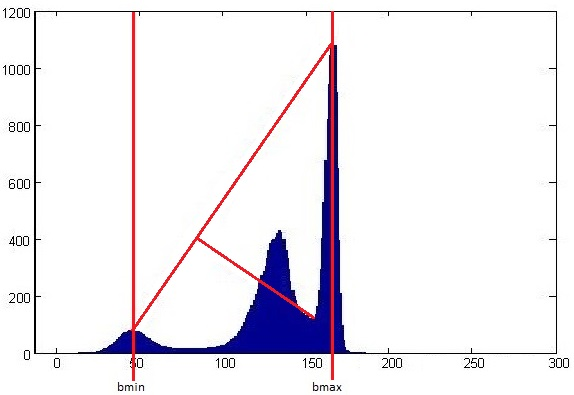
\includegraphics[width=0.57\textwidth]{images/Zack}
\caption{\label{fig:exampleZack}Example of Zack algorithm.}
\end{figure}

\subsection{Fuzzy Threshold} % DONE
The so far treated threshold algorithms are also called crisp techniques. They produce excellent results with well defined images and regions, but the segmentation process becomes complex in presence of noise or imprecision. The nature of this imprecision in the image arises from the presence of uncertainty, that can lead to ill-defined regions. In this case it is appropriate to avoid crisp segmentation and to prefer a fuzzy segmentation. Fuzzy threshold approaches are based on Fuzzy Sets (\acs{FS}s) theory, in fact regions may be viewed as fuzzy subsets of the image. Several researchers have worked on fuzzy based thresholding techniques, in particular in order to identify the best fuzzy measure able to separate the fuzzy subset, such as the fuzzy compactness \cite{Pal}, the fuzzy similarity \cite{Ramar} or the fuzzy divergence and gamma membership \cite{Cha03, MeloP}.
Fuzzy threshold approaches segmentation performances are better than many crisp methods even though their computational performances are not comparable. As a matter of fact, crisp methods are entirely based on computations performed on the histogram, a 1-D array easily obtainable from the image, while fuzzy approaches are based on computations performed on the image, a 2-D array of size $M \times N$.

\subsection{Local Thresholding} \label{LT} % DONE
When the background is not constant and the contrast of the objects varies unevenly, the global thresholding can work properly in an area, but produces unsatisfactory results in other areas. In this case the use of local thresholding could be a better solution. The image is subdivided into rectangular overlapping sub-images and the histogram of each of them is calculated. The sub-images must be big enough to include both the object and the background pixels. If the sub-image has a bimodal histogram, the minimum value between the two peaks is precisely the threshold. If the histogram is unimodal, the threshold value must be calculated by interpolating the thresholds of the adjacent sub-images, instead. In general, the local thresholding is computationally more expensive than the global one, although it is very useful to segment objects from the background and to extract very small and scattered variable regions.

\section{Edge Based} % DONE
This segmentation technique is not based on the intensity value of the pixels, but on the fact that an object to be identified must have a closed edge that surrounds it. This assumption is not always true, but often verified. The edges of objects are preliminarily identified by applying suitable operators of edge detection. As said previously, an edge is a set of connected pixels (4 or 8 connected) that lies on the border of two regions, therefore presenting sharp brightness changes. There is a little difference between edge and boundary, since the edge is a local concept while the boundary is an extended concept. So, it can be said that the boundary of an object is composed of a series of edges.
In order to detect only the edge, it is possible to carry out a threshold applied to the first derivative, an operation that takes the name of non-maxima suppression, as it resets all the values ​​in the first derivative which are not maximum. Actually, the chosen threshold value allows to select more than one maximum points, as to have a contour wider but visible. Instead, if the operation of threshold is applied to the second derivative, this operation takes the name of zero crossing and has the aim of seeking zero crossing points, necessary for the location of the edge points without distortion, avoiding the appearance of a double border. As previously mentioned, there are several implementations of filters on the first derivative, that can be applied directly to the search of the edges. In general, before the edge detection, a smoothing filter is applied to the image, in order to reduce both the noise and the edge thickness, so that the detection is more effective. In fact, the process works perfectly if the signal is not noisy and if the edge is quite localized in space and with small amplitude. An evolution of this approach are the Laplacian of Gaussian (\acs{LoG}) filter with zero crossing and the Canny filter with non-maxima suppression.

\subsection{LoG Operator} % DONE
This edge detection approach, also known as Marr-Hildreth algorithm \cite{Marr}, is based on the second derivative of a function. The Laplacian operator is rarely used by itself for edge detection, as it is very sensitive to noise, but it is used in conjunction with the Gaussian one, known precisely as Laplacian of Gaussian, LoG. The fundamental characteristics of LoG are the Gaussian smoothing filter, used to reduce noise and to enlarge the edge, the Laplacian in two dimensions, the zero crossings in the second derivative and, finally, the edge location estimated with sub-pixel using the linear interpolation. The Gaussian filter is preferred because it applies an action of smoothing both in space and in frequency. Furthermore, the derivative of the Gaussian filter is independent from the considered image and can be pre-calculated analytically by reducing complexity. Once the Laplacian filter is applied, it is needed to search points in the image in which there is a zero crossing, considering only those zeros for which there is a sign change in all possible directions around zero.

\subsection{Canny Operator} % DONE R
Even the Canny algorithm \cite{Canny} uses a Gaussian filter for smoothing. Then the magnitude and direction of the gradient is calculated using different but finite approximations of partial derivatives. It applies the non maxima suppression to the magnitude of the gradient and finally it uses the double threshold algorithm to find and link the edges. The use of the double threshold is necessary, considering that a single threshold would not lead to satisfactory results. For example if the threshold is too low it may detect too many false edges, instead if the threshold is too high some real edges may be lost. The use of two thresholds produces two different images and, of course, the image with the higher threshold will present a much smaller number of edges. Starting from this image each edge is examined and compared with that one of the other image in search of edges that have been lost and that can be linked to create a continuous boundary.

\subsection{Deformable Models} % DONE
In medical image analysis, in many cases, the boundaries between the tissue structures and cell components are not clearly defined. The use of edge detection on these images produces poor results, in particular due to the presence of small structures or particles this approach produces a huge number of false edges. Moreover, in general, the edge approaches based on filters do not yield to a closed contour. As a result, these techniques either fail completely or require some kind of post-processing step to remove invalid object boundaries in the segmentation results or to close the extracted contour. To address these difficulties, deformable models or snakes \cite{Kass} have been extensively studied and widely used in medical image segmentation, with promising results. Deformable models are curves or surfaces defined to match a contour as an energy minimization problem, where the optimal solution constitutes an equilibrium of internal and external energy. The deformable model can move under the influence of internal forces, which are defined within the curve or surface itself to keep the model smooth during deformation, while external forces, which are computed from the image data, are defined to move the model toward an object boundary or other desired features within an image. By constraining extracted boundaries to be smooth and incorporating other prior information about the object shape, deformable models offer robustness to both image noise and boundary gaps.

\section{Region Based} % DONE
These segmentation techniques introduce more information than previous concerning the connectivity of the pixels forming the entire object, avoiding in this way that individual points of a same region, having the right colour or the right contrast, are classified as separate objects. Unlike the pixel and edge based segmentation methods, region based approaches aim to identify objects and regions, working directly on the space occupied by the pixels instead of identifying objects from their properties, such as brightness or edges. Considering $R$ as the entire spatial region occupied by the image, the segmentation process can be seen as the partitioning of $R$ into $n$ sub-regions $R1, R2, ..., Rn$, with the constraint that, the union of all regions returns $R$ and the intersection between any set of regions is equal to $0$. The pixels belonging to a region must be connected (8 or 4 connected) and they must be related by a similarity criterion. The most common techniques of segmentation region based are divided into region growing and split and merge techniques.

\subsection{Region Growing} % DONE
The region growing is a procedure that allows to select regions connected and homogeneous of an image, whose selection is effected from a single pixel and is based on a similarity or growth criterion which imposes a maximum difference, a priori defined, between the value of the initial pixel and the pixel values ​​of the region. The basic approach involves the selection of a set of starting pixels, called seed points, and from these seeds add the pixels of their neighbourhood that have certain properties of similarity with the seeds, such a specific intensity range or colour. The selection of the set of starting pixels is based on the nature of the problem, instead the selection criteria of similarity depends both on the problem and the type of the input image, since it must be ensured independence between the result of the segmentation and the scan direction of the image or the selected seed points. 

Algorithms of region growing have been widely used for the analysis of peripheral blood images, in particular for segmentation of cells in which the nucleus is easily identifiable and thus can be used as a seed. 

\subsection{Split and Merge} % DONE
Segmentation can be performed also by recursively splitting (partitioning) an image, until uniform regions are obtained. Then, merging (aggregation) can be performed on adjacent regions that may be compatible on the basis of a similarity criterion. In the simplest way an image can be partitioned recursively repeating a division into four quadrants, until uniform smaller regions (even composed of a few pixels) have been obtained, according to the defined similarity criterion. Such division into quadrants is represented by a tree called quad-tree, in which the root node contains the information of the whole image and each of the four children nodes contains the information about a quadrant. If a quadrant is sufficiently uniform, it will not be further partitioned. Splitting step inevitably partitions also homogeneous regions and makes necessary a subsequent phase to merge the adjacent and homogeneous regions of the image into a region that meets the defined criterion of similarity.

\subsection{Watershed} \label{watershed} % DONE
The watershed segmentation \cite{Meyer} is a mixed approach based on the pixel aggregation (flooding) with the use of the image gradient as a barrier for flooding. In this approach the gradient image can be considered as a topographical 3D image, in which it is possible to identify points that come from a regional minimum, points that surely fall in a local minimum called basin and points of local maximum called watershed lines. The flooding applied to this image leads to a state where only the watershed lines are visible, that correspond to the objects contours in the image. Actually, a direct application of the watershed algorithm induces an over-segmentation due to the presence of too many basins which can never merge, or the presence of noise and other irregularities of the gradient. In order to avoid this problem in digital microscopy images analysis, watershed is often used with different strategies that include the use of markers. These markers can be extracted directly from the original images intensity value and subsequently combined with the gradient to obtain a stronger result.

\section{Post-Processing} \label{postp}
After segmentation, an image can be represented as a map of binary objects, background and foreground. In some cases, the initial segmentation is not satisfactory, as it can present holes or artefacts. Some improvements to the segmentation results can be made directly on the binary image using a series of operations based on an a priori knowledge. The morphological operators are commonly used for this purpose, to reduce the number of artefacts, to fill the holes present in some regions, to remove some objects not completely enclosed in the image or others that are not interesting for the analysis. Mathematical morphology is based on set theory for binary images \cite{Serra, Serra2} and on lattice theory for grey level images. It provides some approaches for image processing that are useful to extract image components and for the representation and description of the objects shape. The sets, in this case, represent the objects contained in the image. The operations of mathematical morphology are based on the use of structuring elements, that are small sets of sub-images used to investigate and study the properties of interest in the input image. They can have any shape defined according to the problem to be treated and are represented as binary matrices.

\subsection{Mathematical morphology} % DONE
Mathematical morphology (MM) can be defined as a theory for the analysis of spatial structures. It is called morphology because it aims at analysing the shape and form of objects. It is mathematical in the sense that the analysis is based on set theory, integral geometry, and lattice algebra. MM is not only a theory, but also a very powerful image analysis technique \cite{Soille2004}.
It was introduced by Matheron in 1964 as a technique for analysing geometric structure of metallic and geologic samples. It refers to a branch of nonlinear image processing and analysis that concentrates on the geometric structure within an image.
The morphological filters, which can be constructed on the basis of the underlying morphological operations, are more suitable for shape analysis than the standard linear filters since the latter sometimes distort the underlying geometric form of the image. Some of the salient points regarding the morphological approach are as follows \cite{Giardina1988}:
\begin{itemize}
	\item Morphological operations provide for the systematic alteration of the geometric content of an image while maintaining the stability of the important geometric characteristics.
	\item There exists a well-developed morphological algebra that can be employed for representation and optimization.
	\item It is possible to express digital algorithms in terms of a very small class of primitive morphological~operations.
	\item There exist rigorous representation theorems by means of which one can obtain the expression of morphological filters in terms of the primitive morphological operations.
\end{itemize}

MM was initially developed for binary images and later on generalized to grayscale images \cite{Soille2004,Serra1984}, considered as a sampled function of $\mathbb{R}^{2}$ in $\mathbb{R}$, or in general of any function of $\mathbb{R}^{n}$ in $\mathbb{R}$.
More recently, several researchers have extended morphological operators to colour (or in general multispectral) images, considered as sampled functions of $\mathbb{R}^{n}$ in $\mathbb{R}^{m}$, with $m$ being equal to three in the case of the usual colour images or to the number of bands otherwise \cite{Benavent2012}.  Moreover, several approaches for fuzzifying MM have been proposed, extending the ordinary  morphological operations by using fuzzy sets \cite{Kerre2000}.

Dilation and erosion are the basic morphological processing operations. They are defined in terms of more elementary set operations, but are employed as the basic elements of many algorithms. Both~dilation and erosion are produced by the interaction of a set called structuring element (SE) with a set of pixels of interest in the image. The structuring element has both a shape and an origin. From these two basic operators, others have been derived (opening, closing, hit-or-miss). They can be applied to extract image components useful in the representation and descriptions of region shapes, such as area granulometry, boundaries, skeleton, or convex hull. In addition, morphological operators can be used for image preprocessing and postprocessing, such as morphological filtering, thinning, and~especially for segmentation.

Given an image or set $A$ and a structuring element $B$, the operations are realized by sliding $B$ over $A$ so that the origin of $B$ visit all elements of $A$. The \textit{erosion} operation creates a new set by considering all the location of $B$ for which $B$ is fully contained in $A$. The result is that the contour of the set $A$ has been eroded. Such a property for which $B$ must be fully contained in $A$ is equivalent to the property for which $B$ must not share any elements with the complement of $A$. The erosion and dilation are dual operations, thus it is possible to obtain the dilation of $A$ through the use of a structuring element $B$ eroding the complement of $A$. In a more direct way, the \textit{dilation} operation creates a new set by considering all the location of $B$ for which at most one element of $B$ is contained in $A$. The result is that the contour of the set $A$ has been dilated. A simple operation that arises from the erosion is the \textit{boundary extraction}. In fact the contour of a set $A$ can be obtained from the difference between the original set $A$ and the erosion of $A$ with an appropriate structuring element $B$.

Also the opening and closing arise from the composition of erosion and dilation. The \textit{opening} of an image or set $A$ with a structuring element $B$ is defined as the erosion of $A$ with $B$ followed by a dilation of the result. This is useful to flatten the contours of an object, breaking the thin lines and removing the sharp contour. The \textit{closing} of an image or set $A$ with structuring element $B$ is defined as the dilation of $A$ with $B$ followed by the erosion of the result. Even the closing flattens the contours but in a different way, in fact it eliminates small holes and fills the gap in the contours. To fill bigger holes, instead, the operation of \textit{hole filling}, that consists of a more laborious process, is used. Assuming to have a set $A$ with an hole inside, the process starts taking the complement of $A$, that is composed of the background pixels and therefore also the hole pixels. Then, iteratively, a set containing only a pixel for each hole is dilated using an appropriate structuring element and making every time the intersection with the complement of $A$, so as to exclude pixels outside the contour of $A$. In a similar way an iterative procedure of dilatation is used for the \textit{extraction of connected components}. This time the procedure starts from the points of the connected components in $A$, that are dilated until the connected components have been filled. The intersection is performed with $A$ at every iteration, so as to exclude pixels outside the connected component. 

\chapter{Feature Extraction} % DONE
Once the image has been segmented into regions, the collection of resulting segmented pixels is represented and described appropriately for further processes. The representation of a region may be based on external characteristics, such as the contour and shape or internal characteristics, such as the colour and displacement of the pixels inside the region. The following step results to be the description of the regions according to the chosen representation. In peripheral blood cells images analysis, it may be necessary to use both representations, as it is important to analyse characteristics such as shape and area of a cell and also regional characteristics such as colour and texture. The features must be extracted from the object in order to describe it.
The ideal descriptors are those independent to transformation such as the orientation of the object, size and position and that are sufficiently discriminatory. The purpose of the phase of feature extraction is to obtain a set of descriptors, that will be further separated into different classes by a classification procedure. Features are classified into two distinct groups:
\begin{itemize}
\item general features: application independent features such as colour, texture and shape. They can be further divided into features calculated at each pixel, like colour and location (\textit{pixel-level features}), features calculated over the results of segmentation or edge detection (\textit{local features}) and features calculated over the entire image or sub-image (\textit{global features}).
\item domain-specific features: application dependent features such as human faces, fingerprints and conceptual features.
\end{itemize}
Moreover, all features can be coarsely classified into low-level features and high-level features. Low-level features can be extracted directly from the original images, whereas high-level feature extraction must be based on low-level features. 

\section{Contour Descriptors} % DONE
As previously mentioned, many descriptors may be directly extracted from the segmentation result. For example, one of the simplest descriptors is the \textit{contour length}. A good approximation of the contour length can be easily obtained by counting the pixels of the contour. The value of the \textit{diameter} can be easily obtained by computing the maximum distance between two points of the contour. The segment that connects the end points of the diameter is called the \textit{major axis}, while the \textit{minor axis} is that segment perpendicular to the major axis, of such a length that a rectangle completely encloses the contour, passing through the four points of intersection of the axes. The afore defined rectangle is called \textit{bounding box}, having sides parallel to the two axes. The ratio between the sides of the rectangle or the ratio between the two axes measures the value of \textit{eccentricity} (\ref{eccentricity}). The \textit{elongation} measures how an object is elongated (\ref{elongation}), while \textit{rectangularity} represents how rectangular a shape is or, better, how well it fills its minimum bounding box (\ref{rectangularity}).

\begin{equation}\label{eccentricity}
eccentricity=\frac{\sqrt{(major axis^2 - minor axis^2) }}{major axis}
\end{equation}

\begin{equation}\label{elongation}
elongation=1 - \frac{minor axis}{major axis}
\end{equation}

\begin{equation}\label{rectangularity}
rectangularity=\frac{area}{major axis*minor axis}
\end{equation}

These descriptors are really useful to discriminate the shape of abnormal objects to normal ones, in particular peripheral blood cells given their almost circular shape should be distinguished easily from cells with abnormal shape. 

\section{Regional Descriptors} % DONE
Regional descriptors are the most used, since they provide an overall characterization of the object in exam. Regional descriptors comprise shape, colour and texture descriptors.

\subsection{Geometric Descriptors} % DONE
Geometric descriptors are the most used for peripheral blood cells analysis, since cells differ considerably in size or shape, thus using these descriptors it is possible to easily discriminate them. The simplest geometrical features are area and perimeter, from which it is possible to compute other more complex descriptors. The \textit{area} of a region is defined as the number of pixels that constitute the region. This descriptor can be useful if the visual geometry is fixed and the objects are always analysed approximately at the same distance. \textit{convex area} value is also often used. It is the area of the \textit{convex hull}, the minimum convex polygon that completely encloses the region.
The \textit{perimeter} of a region is defined as the number of pixels of its outline. Even in this case the value of the \textit{convex perimeter} can be used, although it is not usually used as a descriptor, but its most common application is the computation of other descriptors, such as compactness, circularity and convexity. The \textit{compactness} of a region is defined as the ratio between the area of an object and the area of a circle with the same perimeter (\ref{compactness}). The circle is used as a benchmark because it is the most compact form, in fact its value of compactness is $1$. Also the \textit{roundness} calculates the ratio between area and perimeter, however, it excludes the presence of small irregularities. That is the reason why it is calculated from the ratio between region area and that of a circle with the same convex perimeter (\ref{roundness}). The \textit{convexity} instead expresses the relative amount that an object differs from a convex object. This value is obtained through the ratio between the convex perimeter and the perimeter of the object itself (\ref{convexity}). The value of \textit{solidity}, instead, describes the density of an object by comparing the area of an object and the area of its convex hull (\ref{solidity}).

\begin{equation}\label{compactness}
compactness=\frac{4*\pi*area}{perimeter^2}
\end{equation}

\begin{equation}\label{roundness}
roundness=\frac{4*\pi*area}{convex\_perimeter^2}
\end{equation}

\begin{equation}\label{convexity}
convexity=\frac{perimeter_{convex}}{perimeter}
\end{equation}

\begin{equation}\label{solidity}
solidity=\frac{area}{convex\_area}
\end{equation}

All the mentioned descriptors, that is compactness, circularity, convexity and solidity, have a maximum value equal to $1$, indicating that the region is compact, circular, convex and solid, respectively.  The main drawback of the geometric descriptors is that their application requires accurate segmentation of the region of interest and, therefore, they are commonly used with other descriptors less influenced by segmentation errors, such as chromatic descriptors or texture descriptors.

\subsection{Chromatic Descriptors} % DONE
Chromatic descriptors delineate the grey level or colour distribution of images. These descriptors are calculated directly from histograms of the region, which may be considered as functions of colour density. The most used descriptors are the \textit{mean} \ref{hmean},  \textit{standard deviation} (\ref{hsd}), \textit{smoothness} (\ref{hsmo}), \textit{skewness} (\ref{hskew}), \textit{kurtosis} (\ref{hkurt}), \textit{uniformity} (\ref{huni}) and \textit{entropy} (\ref{hent}), that describe the shape of the normalised histogram $h_N$, obtained from the histogram $h$ by dividing each value by the total number of pixels.

\begin{equation}\label{hmean}
\mu=\sum_{k=0}^{N_{g}-1} k\cdot h_N(k)
\end{equation}

\begin{equation}\label{hsd}
\sigma=\sqrt{v}
\end{equation}

\begin{equation}\label{hsmo}
s=\frac{1}{1 + v/(N_{g}-1)^2 }
\end{equation}

\begin{equation}\label{hskew}
\mu_3=\sigma^{-3} \cdot \sum_{k=0}^{N_{g}-1} (k - \mu)^3 \cdot h_N(k)
\end{equation}

\begin{equation}\label{hkurt}
\mu_4 =\sigma^{-4} \cdot \sum_{k=0}^{N_{g}-1} (k - \mu)^4 \cdot h_N(k)
\end{equation}

\begin{equation}\label{huni}
uni=\sum_{k=0}^{N_{g}-1} h_N ^2 (k)
\end{equation}

\begin{equation}\label{hent}
e=-\sum_{k=0}^{N_{g}-1}  h_N(k) \cdot  log_2(h_N(k))
\end{equation}

where $v$ is the \textit{variance} value (\ref{hvar}). 

\begin{equation}\label{hvar}
v=\sum_{k=0}^{N_{g}-1} (k - \mu)^2 \cdot h_N(k)
\end{equation}

The chromatic descriptors are the most discriminatory characteristics between different types of tissues and cells, but generally the discrimination on sub-classes requires further descriptors such as texture measures.

\subsection{Texture Descriptors} % DONE
The traditional machine vision and image processing approaches assume the presence of uniform intensity values in local regions of the image. This assumption is not always true, in fact some objects have a repeated pattern as the main visual feature, which is called texture. Texture probably represents the most used descriptor for the description of the regions of images. Although there are no formal definitions of what is a texture, it can be viewed as a global descriptor generated from the repetition of local patterns. A texture basically is a repetitive geometric arrangement of the grey levels of an image. It provides important information about the spatial disposition of the grey levels and the relationship with their neighbourhoods. Human visual system determines and recognizes easily different types of textures but although for a human observer associating a surface with a texture is very simple, giving a rigorous definition for this is very complex. Typically, a qualitative definition is used to describe textures. It can be easily guessed that the quantitative analysis of texture passes through statistical and structural relationships among the basic elements of what we simply call texture. Intuitively, texture descriptors provide measures of properties such as regularity, smoothness, roughness, coarseness, thickness, and so on. In medical image analysis, texture descriptor has proven itself useful to distinguish some abnormal cells or the presence of parasites in the process of evolution. The most used approach for the description of the texture is the statistical approach, that is also the simplest for texture representation. There are many statistical descriptors that use statistical moments extracted from the histogram of the image or the region. The measures of texture based only on histograms, however, have many drawbacks. In particular statistical moments do not give information about the mutual position of the pixels. Thus, it is important to consider not only the intensity distribution but also the positions of pixels having similar grey levels. Many different methods for managing textures have been developed and are based on the various ways texture can be characterized, including the scale-invariant feature transform (SIFT) \cite{Lowe}, speeded up robust feature (SURF)\cite{Bay}, histogram of oriented gradients (HOG) \cite{Dalal}, Gabor filters \cite{Jain} and others.

\subsubsection{Gray Level Co-occurrence Matrix} \label{GLCM}
One of the most powerful model for texture analysis was proposed by Haralick \cite{Haralick}. His method involves the creation of the Gray Level Co-occurrence Matrices (\acs{GLCM}s) from which features that represent some image aspects can be calculated. A GLCM represents the probability of finding two pixels \textit{i} and \textit{j} with distance \textit{d} and orientation $\theta$ and it is denoted with $p_{d,\theta}(i,j)$. Obviously, the \textit{d} and $\theta$ values can assume different values, but the most used are $d = 1$ and $\theta = [0 ^\circ, 45 ^\circ, 90 ^\circ, 135 ^\circ]$. A GLCM for an image of size $N \times M$ with $N_{g}$ grey levels is a 2D array of size $N_{g} \times N_{g}$. Haralick proposed thirteen descriptors that can be extracted from these matrices. 

\noindent\textit{Angular Second Moment}: is the squares sum of the matrix values (\ref{asm}). It is also known as Uniformity. This feature has a range between 0 and 1. The value is 0 if the image is constant.\\
\begin{equation}\label{asm}
\acs{ASM}=\sum_{i=0}^{N_{g}-1}\sum_{j=0}^{N_{g}-1}p(i,j)^2
\end{equation}
Often it is called also \textit{Energy} but it is calculated as in (\ref{Energy}).
\begin{equation}\label{Energy}
\acs{Ene}=\sqrt{\sum_{i=0}^{N_{g}-1}\sum_{j=0}^{N_{g}-1}p(i,j)^2}
\end{equation}
\textit{Contrast}: is the weighted average of all diagonals parallel to the main one which emphasizes the correlation between the different tones (\ref{contrast}). The contrast is 0 if the image is constant.
\begin{equation}\label{contrast}
\acs{Con}=\sum_{i=0}^{N_{g}-1}\sum_{j=0}^{N_{g}-1} (i-j)^2 \cdot p(i,j)
\end{equation}
\textit{Correlation}: is the measure of how a pixel is in correlation with its neighbours across the image. It is 1 or -1 for an image related perfectly positively or negatively. It is 0 if the image is constant (\ref{correlation}).
\begin{equation}\label{correlation}
\acs{Cor}=\sum_{i=0}^{N_{g}-1}\sum_{j=0}^{N_{g}-1}  \frac{(i-\mu_x) \cdot (j-\mu_y) \cdot p(i,j)}{\sigma_x \cdot \sigma_y}
\end{equation}
\textit{Variance}: is the measure of linear dependence of the brightness determined from the correlation (\ref{variance}).
\begin{equation}\label{variance}
\acs{Var}=\sum_{i=0}^{N_{g}-1}\sum_{j=0}^{N_{g}-1}(i-\mu)^2 \cdot p(i,j)
\end{equation}
\textit{Inverse Difference Moment}: is a value which measures the proximity of the distribution from GLCM elements to the GLCM diagonal. It has value 1 in the main diagonal of its GLCM (\ref{IDM}).
\begin{equation}\label{IDM}
\acs{IDM}=\sum_{i=0}^{N_{g}-1}\sum_{j=0}^{N_{g}-1}\frac{p(i,j)}{1 + (i-j)^2}
\end{equation}
Often it is called also \textit{Homogeneity} and is calculated as in (\ref{Homogeneity}).
\begin{equation}\label{Homogeneity}
\acs{Hom}=\sum_{i=0}^{N_{g}-1}\sum_{j=0}^{N_{g}-1}\frac{p(i,j)}{1 + |i-j|}
\end{equation}
\textit{Sum Average}: is the average of the value $p_{x+y}$ containing the sums of all the diagonal orthogonal to the main (\ref{sumAverage}).
\begin{equation}\label{sumAverage}
\acs{SAve}=\sum_{k=0}^{2N_{g}-2}k\cdot p_{x+y}(k)
\end{equation}
\textit{Sum Variance}: is an estimation of the second order of the vector $p_{x+y}$ centralized respect to the average (\ref{sumVariance}).
\begin{equation}\label{sumVariance}
\acs{SVar}=\sum_{k=0}^{2N_{g}-2}(k - F_{SAv})^2 \cdot p_{x+y}(k)
\end{equation}
\textit{Sum Entropy}: provides an estimate of the vector $p_{x+y}$ relative to entropy, which is the measure of the disorder of the vector itself (\ref{sumEntropy}).
\begin{equation}\label{sumEntropy}
\acs{SEnt}=-\sum_{k=0}^{2N_{g}-2}p_{x+y}(k)\cdot log_2(p_{x+y}(k))
\end{equation}
\textit{Entropy}: is the entropy measure for the entire matrix (\ref{entropy}).
\begin{equation}\label{entropy}
\acs{Ent}=-\sum_{i=0}^{N_{g}-1}\sum_{j=0}^{N_{g}-1} p(i,j)\cdot log_2(p(i,j))
\end{equation}
\textit{Difference Variance}: is the variance of the vector $p_{x-y}$ (\ref{diffVariance}).
\begin{equation}\label{diffVariance}
\acs{DVar}=\sum_{k=0}^{N_{g}-1}(k - F_{DAv})^2 \cdot p_{x-y}(k)
\end{equation}
where \acs{DAve}, \textit{Difference Average} or \textit{Dissimilarity}, is the average of the vector $p_{x-y}$ containing the differences of all the diagonal orthogonal to the main (\ref{diffAverage}).

\noindent\textit{Difference Entropy}: is the entropy measure of the vector $p_{x-y}$ (\ref{diffEntropy}).
\begin{equation}\label{diffEntropy}
\acs{DEnt}=-\sum_{k=0}^{N_{g}-1}p_{x-y}(k) \cdot log_2(p_{x-y}(k))
\end{equation}
\textit{Measure of correlation 1 and 2}: are measures related to entropy of the matrix (\ref{MIC1}),(\ref{MIC2}).
\begin{equation}\label{MIC1}
\acs{MC}1=\frac{F_{Ent} - HXY1}{max(Hx-Hy)}
\end{equation}
\begin{equation}\label{MIC2}
\acs{MC}2=\sqrt{1-exp[-2(HXY2-F_{Ent})]}
\end{equation}
where
\begin{equation}\label{Px}
p_{x}(i)=\sum_{j=0}^{N_{g}-1} p(i,j) 
\end{equation}
\begin{equation}\label{Py}
p_{y}(j)=\sum_{i=0}^{N_{g}-1} p(i,j) 
\end{equation}
\begin{equation}\label{Px-y}
p_{x-y}(i-j)=\sum_{i=0}^{N_{g}-1} \sum_{j=0}^{N_{g}-1} p(i,j) 
\end{equation}
\begin{equation}\label{Px+y}
p_{x+y}(i+j)=\sum_{i=0}^{N_{g}-1} \sum_{j=0}^{N_{g}-1} p(i,j) 
\end{equation}
\begin{equation}\label{MUx}
\mu_x=\sum_{i=0}^{N_{g}-1} i \cdot p_x(i) 
\end{equation}
\begin{equation}\label{MUy}
\mu_y=\sum_{j=0}^{N_{g}-1} j \cdot p_y(j) 
\end{equation}
\begin{equation}\label{MU}
\mu=(\mu_x+\mu_y)/2 
\end{equation}
\begin{equation}\label{Sigmax}
\sigma_x=\sqrt{\sum_{i=0}^{N_{g}-1} p_x(i) \cdot (i-\mu_x)^2} 
\end{equation}
\begin{equation}\label{Sigmay}
\sigma_y=\sqrt{\sum_{j=0}^{N_{g}-1} p_y(j) \cdot (j-\mu_y)^2} 
\end{equation}
\begin{equation}\label{hx}
HX=-\sum_{i=0}^{N_{g}-1}p_{x}(i) \cdot log_2(p_{x}(i))
\end{equation}
\begin{equation}\label{hy}
HY=-\sum_{j=0}^{N_{g}-1}p_{y}(j) \cdot log_2(p_{y}(j))
\end{equation}
\begin{equation}\label{hxy1}
HXY1=-\sum_{i=0}^{N_{g}-1}\sum_{j=0}^{N_{g}-1}p(i,j) \cdot log_2(p_{x}(i) \cdot p_{y}(j))
\end{equation}
\begin{equation}\label{hxy2}
HXY2=-\sum_{i=0}^{N_{g}-1}\sum_{j=0}^{N_{g}-1}p_{x}(i) \cdot p_{y}(j) \cdot log_2(p_{x}(i) \cdot p_{y}(j))
\end{equation}

To these descriptors extracted from GLCMs many others have been proposed, but only seven are widely used \cite{Soh, Clausi}, that are \textit{mean} (\ref {Mean}), \textit{difference average} (\ref{diffAverage}), \textit{autocorrelation} (\ref{Aut}), \textit{maximum probability} (\ref{MP}), \textit{cluster shade} (\ref{ClustShade}),  \textit{cluster prominence} (\ref {ClustProm}) and \textit{product moment} (\ref {ProdMom}). 

\begin{equation}\label{Mean}
{\mu}=\sum_{i=0}^{N_{g}-1}\sum_{j=0}^{N_{g}-1} i \cdot p(i,j)
\end{equation}

\begin{equation}\label{diffAverage}
\acs{DAve}= \sum_{i=0}^{N_{g}-1}\sum_{j=0}^{N_{g}-1}  |i-j| \cdot p(i,j) = \sum_{k=0}^{N_{g}-1} k \cdot p_{x-y}(k)
\end{equation}

\begin{equation}\label{Aut}
\acs{Aut}=\sum_{i=0}^{N_{g}-1}\sum_{j=0}^{N_{g}-1} i \cdot j \cdot p(i,j)
\end{equation}

\begin{equation}\label{MP}
\acs{MP}=max(p(i,j))
\end{equation}

\begin{equation}\label{ClustShade}
\acs{CS}=\sum_{i=0}^{N_{g}-1}\sum_{j=0}^{N_{g}-1}  (i + j - \mu_x - \mu_y)^3 \cdot p(i,j)
\end{equation}

\begin{equation}\label{ClustProm}
\acs{CP}=\sum_{i=0}^{N_{g}-1}\sum_{j=0}^{N_{g}-1}  (i + j - \mu_x - \mu_y)^4 \cdot p(i,j)
\end{equation}

\begin{equation}\label{ProdMom}
\acs{PM}=\sum_{i=0}^{N_{g}-1}\sum_{j=0}^{N_{g}-1}  (i - \mu_x) \cdot (j - \mu_y) \cdot p(i,j)
\end{equation}

Some interesting methods have also been presented in order to extend the original implementation of GLCM, computing the matrices by evaluating different distance parameters \cite{Gelz}, different windows sizes \cite{HuY}, different colour channels \cite{Benco}, adding the colour gradient \cite{Gong} or considering also the edge orientation \cite{Mitrea}. Furthermore the GLCM descriptors can be extracted after computing a weighted sum of GLCM elements \cite{Walker} or after computing the local gradient of the matrix \cite{Chen}. 

\subsubsection{Gray Level Difference Matrix} \label{GLDM}
Another useful tool for texture analysis is the grey level difference matrix (\acs{GLDM})\cite{Conners}, that is a particular type of matrix originated by the absolute differences between grey levels pairs. Actually, the GLDM is defined in very similar way to the GLCM, using the same notions of distance and orientation to find grey levels pairs. The main difference arises in the construction and dimension of the matrix. In fact, the GLDM preserves the size of the original image (and not $N_{g} \times N_{g}$), collecting the absolute difference between pairs of pixel values (and not the occurrences of two grey levels). This matrix is used to calculate the histogram $h(d)$ that denotes the number of differences with value $d$. The histogram is then normalized $h_N(d)=h(d)/N $ with $N = \sum_{d} h(d)$ in order to easily compute nine descriptors
that are \textit{mean} (\ref {meanGLDM}), \textit{angular second moment} (\ref{asmGLDM}), \textit{contrast} (\ref{contrastGLDM}), \textit{variance} (\ref{varianceGLDM}), \textit{inverse difference moment} (\ref{IDMGLDM}),  \textit{entropy} (\ref {entropyGLDM}), \textit{product moment} (\ref {PMGLDM}), \textit{cluster shade} (\ref{CSGLDM}) and \textit{cluster prominence} (\ref {CPGLDM}). 

\noindent\textit{Mean}:
\begin{equation}\label{meanGLDM}
\mu=\sum_{d=0}^{N_{g}-1} d \cdot h_N(d)
\end{equation}
\textit{Angular Second Moment}:
\begin{equation}\label{asmGLDM}
ASM=\sum_{d=0}^{N_{g}-1} h_N(d)^2
\end{equation}
\textit{Contrast}:
\begin{equation}\label{contrastGLDM}
Con=\sum_{d=0}^{N_{g}-1} d^2 \cdot h_N(d)
\end{equation}
\textit{Variance}:
\begin{equation}\label{varianceGLDM}
Var=\sum_{d=0}^{N_{g}-1} (d - \mu)^2 \cdot h_N(d)
\end{equation}
\textit{Inverse Difference Moment}:
\begin{equation}\label{IDMGLDM}
IDM=\sum_{d=0}^{N_{g}-1}  \frac{h_N(d)}{1 + d^2}
\end{equation}
\textit{Entropy}:
\begin{equation}\label{entropyGLDM}
Ent=\sum_{d=0}^{N_{g}-1} h_N(d) \cdot log_2(h_N(d))
\end{equation}
\textit{Product Moment}:
\begin{equation}\label{PMGLDM}
PM=\sum_{d=0}^{N_{g}-1}  (d - \mu) \cdot h_N(d)
\end{equation}
\textit{Cluster Shade}:
\begin{equation}\label{CSGLDM}
CS=\sum_{d=0}^{N_{g}-1}  (d - \mu)^3 \cdot h_N(d)
\end{equation}
\textit{Cluster Prominence}:
\begin{equation}\label{CPGLDM}
CP=\sum_{d=0}^{N_{g}-1}  (d - \mu)^4 \cdot h_N(d)
\end{equation}

\subsubsection{Gray Level Run-Length Matrix} \label{GLRLM}
A different tool for texture analysis is based on information of higher order statistics that uses the Grey Level Run-Length Matrices (\acs{GLRLM}) \cite{Tang}. In this approach the GLRLM contains information on a particular number of equal grey levels (run) in a given direction. So, a run-length matrix is defined as a set of consecutive pixels having the same grey level. The element $(i, j)$ of a run-length matrix specifies the number of times that the image contains a run of length $j$ composed by all pixels with grey level $i$. The creation of the run-length matrices is very simple and the number of operations to be done is directly proportional to the number of image points. A coarse texture will be characterized by a long run, while a finer texture will be characterized by a shorter run. Also, the GLRLMs are calculated by considering the main four orientations and for each matrix eleven descriptors can be extracted, that are \textit{short run emphasis} (\ref {SRE}), \textit{long run emphasis} (\ref{LRE}), \textit{grey level non-uniformity} (\ref{GLN}), \textit{run length non-uniformity} (\ref{RLN}), \textit{run percentage} (\ref{RP}),  \textit{low grey level run emphasis} (\ref {LGLRE}), \textit{high grey level run emphasis} (\ref {HGLRE}), \textit{short run low grey level emphasis} (\ref{SRLGLE}), \textit{short run high grey level emphasis} (\ref{SRHGLE}), \textit{long run low grey level emphasis} (\ref{LRLGLE}) and \textit{long run high grey level emphasis} (\ref {LRHGLE}). 

\noindent\textit{Short Run Emphasis}:
\begin{equation}\label{SRE}
\acs{SRE}=  \frac{1}{n_r} \sum_{i=1}^{M} \sum_{j=1}^{N}  \frac{p(i,j)}{j^2} = \frac{1}{n_r} \sum_{j=1}^{N}  \frac{p_r(j)}{j^2} 		 
\end{equation}

\noindent\textit{Long Run Emphasis}:
\begin{equation}\label{LRE}
\acs{LRE}=  \frac{1}{n_r} \sum_{i=1}^{M} \sum_{j=1}^{N} p(i,j) \cdot j^2 = \frac{1}{n_r} \sum_{j=1}^{N} p_r(j) \cdot j^2 		 
\end{equation}
 
\noindent\textit{Grey Level Non-uniformity}
\begin{equation}\label{GLN}
\acs{GLN}=  \frac{1}{n_r} \sum_{i=1}^{M} \left(  \sum_{j=1}^{N} p(i,j)  \right)^2 = \frac{1}{n_r} \sum_{i=1}^{M} p_g(i)^2 		 
\end{equation}

\noindent\textit{Run Length Non-uniformity}
\begin{equation}\label{RLN}
\acs{RLN}=  \frac{1}{n_r} \sum_{j=1}^{N} \left( \sum_{i=1}^{M} p(i,j) \right)^2 = \frac{1}{n_r} \sum_{j=1}^{N} p_r(j)^2 		 
\end{equation}

\noindent\textit{Run Percentage}
\begin{equation}\label{RP}
\acs{RP}=  \frac{n_r}{n_p} 		 
\end{equation}

\noindent\textit{Low Grey Level Run Emphasis} 
\begin{equation}\label{LGLRE}
\acs{LGLRE}=  \frac{1}{n_r} \sum_{i=1}^{M} \sum_{j=1}^{N}  \frac{p(i,j)}{i^2} = \frac{1}{n_r} \sum_{i=1}^{M}  \frac{p_g(i)}{i^2} 		 
\end{equation}

\noindent\textit{High Grey Level Run Emphasis}
\begin{equation}\label{HGLRE}
\acs{HGLRE}=  \frac{1}{n_r} \sum_{i=1}^{M} \sum_{j=1}^{N}  p(i,j) \cdot i^2 = \frac{1}{n_r} \sum_{i=1}^{M} p_g(i) \cdot i^2 		 
\end{equation}

\noindent\textit{Short Run Low Grey Level Emphasis}
\begin{equation}\label{SRLGLE}
\acs{SRLGLE}=  \frac{1}{n_r} \sum_{i=1}^{M} \sum_{j=1}^{N}  \frac{p(i,j)}{i^2 \cdot j^2}		 
\end{equation}

\noindent\textit{Short Run High Grey Level Emphasis}
\begin{equation}\label{SRHGLE}
\acs{SRHGLE}=  \frac{1}{n_r} \sum_{i=1}^{M} \sum_{j=1}^{N}  \frac{p(i,j) \cdot i^2}{ j^2}		 
\end{equation}

\noindent\textit{Long Run Low Grey Level Emphasis}
\begin{equation}\label{LRLGLE}
\acs{LRLGLE}=  \frac{1}{n_r} \sum_{i=1}^{M} \sum_{j=1}^{N}  \frac{p(i,j) \cdot j^2}{ i^2}		 
\end{equation}

\noindent\textit{Long Run High Grey Level Emphasis}.
\begin{equation}\label{LRHGLE}
\acs{LRHGLE}=  \frac{1}{n_r} \sum_{i=1}^{M} \sum_{j=1}^{N}  p(i,j) \cdot i^2 \cdot j^2		 
\end{equation}

\subsubsection{Local Binary Pattern} \label{LBP}
Another useful tool for texture analysis is the Local Binary Pattern (\acs{LBP}), originally proposed in \cite{Ojala} and widely used for grey level texture classification, due to its simplicity and robustness. This operator transforms the image by thresholding the neighbourhood of each pixel and by coding the result as a binary number. The resulting image histogram can be used as a feature vector for texture classification. Also, for the LBP operator two main parameters must be defined, which are the radius $r$ and the number of neighbourhood $n$ pixels. For example, some possible versions of this operator are the $LBP_{8,1}$ implemented with the parameters $r$ and $n$ equal to 1 and 8, respectively, and the  $LBP_{16,2}$ implemented with the parameters $r$ and $n$ equal to 2 and 16, respectively. These two LBP operators are reported in Fig.\ref{fig:LBP}.

\begin{figure}[!t]
\centering
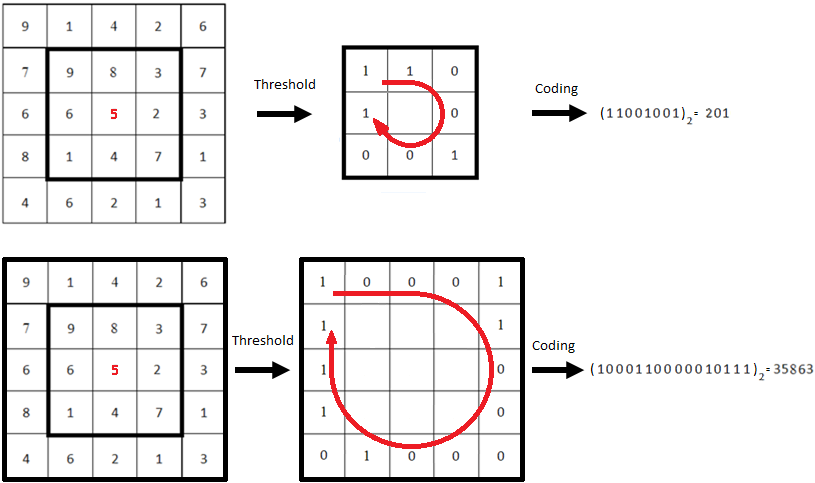
\includegraphics[width=0.90\textwidth]{images/LBP}
\caption{\label{fig:LBP}The LBP operators $LBP_{8,1}$  and $LBP_{16,2}$, respectively  }
\end{figure}

\section{Feature Selection} \label{FS}
A further step, not always present on CAD system, is the feature selection, a process commonly used in pattern recognition that allows to determine the most relevant features reducing the size of the vectors associated with the objects. The feature selection aims to reduce the dimensionality eliminating both the redundant features, that represent information derived from other, both the features that are irrelevant for
the analysis. The "ideal" approach would be to test all the possible sub-sets of features, using them as input to the classification algorithm of interest and select the sub-set that allows to obtain the best results. Obviously this approach in most cases is not applicable. There are several techniques for the selection of characteristics, that can be grouped into three categories:
\begin{itemize}
\item embedded methods: the selection is internal to the classification algorithm that takes advantage of internal knowledge of the classifier, such as the weight used to induce the model \cite{Duda}
\item filter methods: also known as scheme-independent selection, because the selection is made in advance, with a method independent from the classification algorithm that will be applied subsequently using some measure of distance or correlation \cite{Yu}
\item wrapper methods: also known as scheme-specific selection, because the selection is performed making a comparison between different sub-sets of features, investigated with approaches of sequential forward or backward selection \cite{Kittler}, according to the classification algorithm that will be applied later.
\end{itemize}
Generally, the wrapper methods perform better than the other methods, as they are optimized for a specific classifier, but they are computationally eligible only for small feature vectors. On the other hand, there are other approaches called, by many authors, "feature selection" that do not perform a proper features selection, but rather a dimensionality reduction through projection or combination. The Principal Component Analysis (\acs{PCA}) \cite{Wold} is the most popular technique for the reduction of dimensionality. Its purpose is to find a set of orthogonal vectors in the feature space corresponding to the directions along which the data have the highest variance. The dimensionality reduction is performed by projecting the data from their original space to the orthogonal complement. 
The advantages of the PCA is that it can deal with large datasets both in objects and variables reducing the redundancy. Moreover it does not make special assumptions on the data and so it can be applied on all datasets. The biggest disadvantage arises from the fact that PCA does not select the features but it creates new ones combining the original. This greatly affects the control over the single feature, that is particularly important in image processing where features are extracted directly from the image and thus it is important to establish which are determinant for the task of classification, in order to avoid the extraction of insignificant features.  

\chapter{Classification}
Once the features have been extracted from cells they must be inserted in a process that classifies cells based on medical concepts. Given a collection of records, each one composed by a set of features $x$ and by a label of class $y$, the goal is to define a function or classification model, that associates a class label $y$ to each set of attributes $x$. A classification model is a tool to describe and classify the data of a specific domain. This is possible thanks to a training set, namely a set of training samples in which the values ​​of the class labels are well known. So, the relations between attributes and class labels can be identified and encoded in a model, through a learning algorithm. This model must be able not only to describe the training set, but also to correctly predict the class of new records not yet labelled. Literature comprises several classification algorithms, but the most used on medical images are following listed:
\begin{itemize}
\item Nearest Neighbour
\item Decision Trees
\item Bayesian Classifier	
\item Neural Network
\item Support Vector Machine
\end{itemize}

\section{Nearest Neighbour} \label{kNN}
The Nearest Neighbour classifier uses the concept of proximity to classify a new record, based on the samples provided by the training set that are similar to it. Each instance of the training set is represented as a point in an n-dimensional space, where $n$ is the number of features. When NN has to classify a new record, its distance from each training set sample is calculated. Then, the $k$ examples of the training set closer to the new record, called k-Nearest Neighbours (k\acs{NN})  \cite{Cover}, are identified and used to assign the class label prevailing among kNN to the new record. However, there may be problems in the choice of $k$, in fact if this value is too small, there is a high sensitivity to noise, but if it is too large, there may be examples not similar enough to the record to be classified, among the kNN. One way to reduce the influence of the parameter $k$ is to calculate the prevailing class by assigning a different weight to each of the first neighbours according to its distance from the record to be classified. This type of classifier is the simplest among those listed, as it does not require the induction of a model from the training set, which is used in the classification step to compare the new records with the known ones. In contrast to the saved resources for the construction of the model, the classification of a new record, however, is rather expensive. Indeed, the proximity between the new record and the known examples of the training set must be calculated every time.

\section{Decision Trees} \label{DT}
Decision Trees \cite{Quinlan} are decision support tools that use a tree-like graph or decision model for classification. The goal is to create a model that predicts the value of a target variable by learning simple decision rules inferred from the data features. Thus, during the classification of a new record, the decision tree represents a flowchart-like structure in which each internal node represents a test on an attribute and each branch represents the outcome of the test. Obviously, each leaf node represents a class label and the decision is taken after computing all attributes. The paths from the root to the leaf nodes represents the classification rules. The greatest advantage of decision trees is that they are simple to understand and interpret, but they can be really complex with an high number of attributes. In particular, having more attributes conducts to a deeper tree and, therefore, the decision rules become more complex and the model fitter.
Among disadvantages, there is that decision tree can create too complex trees that do not produce a well generalisation of the data, generating overfitting, even though the greatest one is that the same classification rules can be expressed with different decision trees. Thus finding the optimal decision tree is known to be a NP-complete problem under several aspects of optimality and even for simple concepts. This problem is generally mitigated by training multiple trees in an ensemble learner, where the features and samples are randomly sampled with a replacement strategy.

\section{Bayesian Classifier} \label{NB}
The Bayesian classifiers are based on probabilistic relations between the class labels and feature values of the record. Considering the features of a record as random variables a Bayesian network can be used to plot the conditional dependencies among a set of random variables. It is an acyclic and directed graph in which the nodes represent random variables and the arcs represent dependency relationships between the variables. Each node of the network is associated with a probability table containing the a priori probability if that node does not depend on any other node, or the conditional probability if the node depends on a set of other nodes. Thus, given a training sample, it must be found the Bayesian network that best describes the conditional dependencies between variables. Once defined the network, the process of classification of a new record entails the calculation of the posterior probability for each class and the selection of the class for which the probability is the highest. The induction of the network that best describes a given training set involves the definition of network structure and the estimation of probabilities values table associated with each node of the network. In a general case, this is an intractable problem but there are algorithms that induce Bayesian classification models introducing appropriate simplifying assumptions on the network topology. The simplest among the Bayesian classifiers is the so-called Naive Bayes  \cite{Duda}, \cite{Langley} and is based on the assumption that the features are conditionally independent, given the value of the class. In this way the a priori probability of the class and the conditional probabilities of the class features can be easily estimated from the training sample. With the Naive Bayes method, the model is not significantly influenced by either the noise, which is mediated through the calculation of probabilities, or by any irrelevant features, for which the probabilities are distributed in an almost uniform way. Despite its simplicity, the Bayesian classifier is able to perform accurate classifications but only if the features are discriminatory.

\section{Artificial Neural Network} \label{ANN}
Artificial Neural Networks (\acs{ANN}) classifiers are the most used in medical applications. They are networks that emulate the behaviour of the human brain, composed of a set of nodes that are interconnected by links to which a weight is associated. In ANNs, as in biological systems, learning corresponds to change the weight values of the connections between nodes. Given a training sample, the weights of the model are first initialised randomly and then iteratively adjusted, so that the output of the model appears consistent with the values of the label class. The simplest ANNs are composed of two levels, the input level and the output level. The input layer contains a node for each numerical features, while the categorical features require more nodes, for example a feature with $n$ possible values can be transformed into $n$ binary variables. The output layer, on the other hand, can contain only one node, if the problem of classification is binary and $k$ nodes if the class label can assumes $k$ values. There are also multilevel ANNs whose structures present additional hidden layers between the input layer and the output layer. The number hidden layers is often determined by trial and error, in fact typically the correct number of hidden layers is found starting from a network with an high number of layers and nodes and it progressively decreases the model complexity. Network training involves the adjustment of the weights with the aim to minimize the internal error. This process is really expensive, especially if the network topology is complex, even if the classification process is rapid. The model is very sensitive to noise, because the weights are adjusted for each instance of the training sample. On the contrary, the irrelevant or redundant  features do not significantly affect the model, since the corresponding weights are typically very small.

\section{Support Vector Machine} \label{SVM}
Recently, the Support Vector Machine (\acs{SVM}) has received a growing interest in the field of pattern recognition. This technique has been designed for binary classification problems, so with only two classes, but it can also be extended to multi-class problems.The SVM binary classification is based on the mapping of input vectors in an high dimensionality features space, induced by a kernel function. The learning algorithm produces an optimal hyperplane of separation between the two classes. The SVM can perform a linear discrimination, but it can also perform a discrimination not linear due to the use of a kernel function. It is possible to find a kernel function for which the parameters of the model can be induced without an explicit mapping data. The induction of the model in this way is formulated as an optimization problem, in which it is possible to find quite efficiently a global minimum for the objective function. The SVM provides extreme flexibility both because it is possible to make use of different types of kernels and both because it is possible to define a hyperplane for separating classes which guarantees a certain tolerance with respect to noise, using a soft margin instead of an hard margin. This for an optimization problem becomes changing the constraint value with the $c$ value, that can be increased to obtain less training error. Obviously kernel methods use other parameters for the creation of the separating hyperplane. The Gaussian Radial Basis Funcion (\acs{RBF}) is one of the most used kernel performing a non-linear separation defined by the radius  $\gamma$ of the RBF. Other kernels are the quadratic kernel, the polynomial kernel that can be defined with different order $p$ and the Multilayer Perceptron kernel (MLP) that instead can be defined for different slope $\alpha$ and the intercept constant $\beta$. The multi-class problem is solved by building many different binary classifiers and then combine them. The most used strategies are the combinations one-vs-one and one-vs-all. 

\subsection{One-vs-all SVM} 
The one-vs-all, also known as one-vs-rest, approach is the first and the most intuitive approach to extend the SVM to multi-class problems. The basic idea of the one-vs-all approach is very simple. In fact, for a multi-class problem having $m$ classes, it consists on training $m$ different binary SVM classifiers where each one of them separates one class from all the other $m-1$ classes. Then, in testing phase the class label is assigned taking into account the decision of every $m$ classifiers. The most common practice is to assign the class label $i$, where $i$ is the classifier that maximizes the separation between the class $i$ from the rest. Another common practice is to use binary trees to arrange the $m-1$ binary SVM; the path from the root node to a leaf determines the class label. In the best scenario only one comparison is needed, while in the worst case  $m-1$ comparisons are needed. The problem encountered with binary tree SVM is that there are $\prod_{i=3}^{m}2i-3$ possible ways to construct a tree for a multi-class problem. Thus, for a multi-class problem with a very large value of $m$, analysing all the possible solutions is impossible.

\subsection{One-vs-one SVM}
The one-vs-one approach is another commonly used SVM strategy but, differently from the one-vs-all approach, for a multi-class problem having $m$ classes, it consists on training $\frac{m(m-1)}{2}$ different binary SVM classifiers, where each one of them separates a class from another one. In this case, combining the results from individual binary SVM classifiers becomes more complex. The simplest way to obtain the predicted class label is to use the majority voting, counting the votes given by each binary classifier and assigning the class label that has the highest number of votes. However, voting process could produce ambiguous results (eg. tie cases). For this reason, a common practice is to use the majority voting strategy combined with the maximum separation strategy, assigning the class label $i$, if the result of the binary classifier produces the highest number of $i$ votes with the maximum separation between $i$ class and each of the other classes. Another common practice consists in arranging all the $\frac{m(m-1)}{2}$ binary SVM classifiers in a Directed Acyclic Graph (\acs{DAG}) structure with the same number of nodes. The test phase starts at the root node and continues until a leaf node, representing the predicted class label, is reached. Thus, only $m-1$ comparisons are needed, avoiding completely tie cases, but the problem is encountered just during the construction of the DAG. In fact, also in this case, there are several ways to construct the DAG structure and each one of them may produce different classification results and when the number of classes is high, testing all possible orders is impossible.

\section{Model Evaluation} \label{ME} % DONE
The performance of the classification models are then evaluated on the basis of percentage of records correctly classified on a test set with a known class label. Therefore, \textit{accuracy} and the \textit{error rate} of the model can be calculated by comparing the known class labels and the classifiers predicted labels. A binary problem is composed of positive and negative classes and it can be evaluated with the following measures: True Positive (\acs{TP}) indicates the number of positives records correctly classified as positives, True Negative (\acs{TN}) measure indicates the number of negatives records correctly classified as negative, False Positive (\acs{FP}) measure is the number of negative records misclassified as positive and, finally, False Negative (\acs{FN}) measure is the number of positive records misclassified as negative. In this way, the accuracy of the error rate can be written as in (\ref{accuracy}) and (\ref{error}):

\begin{equation}\label{accuracy}
accuracy= \frac{TP + TN}{TP + TN + FP + FN}	
\end{equation}

\begin{equation}\label{error}
error rate= \frac{FP + FN}{TP + TN + FP + FN}	
\end{equation}

Differently from binary classification ones, if the problem presents an uncommon number of classes the accuracy and the error rate typically are not good measures of model performance. In this case, the most used measures are the \textit{True Positive Rate} (\acs{TPR}) also called \textit{sensitivity} or \textit{recall} (r) (\ref{TPR}), the \textit{True Negative Rate} (\acs{TNR}) also called \textit{specificity} (\ref{TNR}), the \textit{False Positive Rate} (\acs{FPR}) (\ref{FPR}), the \textit{False Negative Rate} (\acs{FNR}) (\ref{FNR}) and the \textit{precision} (p) (\ref{precision}). Precision and recall are used if the correct classification of positive instances is considered more important or interesting, according to the faced problem. Indeed, a good model should be able to maximise both these measures. For this reason, another important metric is frequently used: the \textit{F-measure} or \textit{F-score} (\ref{Fmeasure}).

\begin{equation}\label{TPR}
TPR = r = \frac{TP}{TP + FN}	
\end{equation}

\begin{equation}\label{TNR}
TNR = \frac{TN}{TN + FP}	
\end{equation}

\begin{equation}\label{FPR}
FPR= \frac{FP}{TN + FP}	
\end{equation}

\begin{equation}\label{FNR}
FNR= \frac{FN}{TP + FN}	
\end{equation}

\begin{equation}\label{precision}
p = \frac{TP}{TP + FP}	
\end{equation}

\begin{equation}\label{Fmeasure}
F\mbox{-}score = \frac{2rp}{r + p}	
\end{equation}

It is worth noting that the same measures are also used for segmentation evaluation. If any manually segmented images or ground-truth are available, actually, a pixel-wise evaluation can be made in order to assess if a pixel has been correctly included in the region which it belongs (TP), it has been correctly excluded from the region (TN), it has been erroneously included in the region (FP) or it has been erroneously excluded from the region (FN).

The performance of a model may not depend only on the type of classification algorithm but also by other factors such as the size or distribution of the classes in the training and test set. In particular, if the dataset has reduced size the performances are more related to the specific composition of the samples and they are characterized by a higher variance. Some methods are quite useful to extract a representative test set, from the original dataset, able to assess the performance of the model. They are:
\begin{itemize}
\item Holdout: a part of the available samples, the training set, is used to train the model while another part, the test set, is used for its evaluation. This involves a reduction of examples available for training and an addiction due from specific partition created. To ensure that the training set and the test set are uniformly representative, the partition can be made by using a stratified sampling process.
\item Repeated Holdout: the holdout method is iterated $k$ times, in order to avoid the control on the number of times that each record is used for training and testing. The accuracy and error rate are calculated averaging the $k$ iteration results.
\item Cross-Validation: the examples available are divided into $k$ sub-sets of equal dimension. The process of training and evaluation of the model is repeated $k$ times, each time using $k-1$ different sub-sets for training and one sub-set
for the test. As for Repeated Holdout, the accuracy and error rate are calculated averaging the $k$ iteration results, but in this case the final results is more stable since the test sets are mutually exclusive and cover the entire initial sample.
\item Leave-one-out: special case of cross-validation in which $k$ is equal to the number of records.Thus during the training phase the largest possible number of examples is used and each test set contains only one record. This approach provide an exhaustive results but it is computationally very expensive.
\end{itemize}

% DONE

\part{CAD for Peripheral Blood Images} \label{due}

\chapter{Background}

\section{Haematology} % Taken from Sensors Survey DONE
Haematology is the branch of medicine concerned with the study, diagnosis, monitoring, treatment, and prevention of blood and blood-forming organs diseases. Haematology studies the blood in health and pathological conditions, firstly to identify the patient’s health condition and, secondly, to predict how the bone marrow may have contributed to reach that condition. 
Haematology, indeed, studies the relationship between the bone marrow and the systemic circulation. There are many diseases, disorders, and deficiencies that can affect the number and type of produced blood cells, their function and lifespan. Usually, only normal, mature or nearly mature cells are released into the bloodstream, but certain circumstances can induce the bone marrow to release immature and/or abnormal cells into the circulation. The Complete Blood Count (CBC) is one of the most frequently ordered tests to monitor the cell components distribution into the blood stream. It offers various haematologic data represented by the numbers and types of cells in the peripheral blood circulation. The cells percentage is compared with the reference ranges in order to determine if the cells are present in their expected percentage, if one cell type is increased, decreased or if immature cells exist. Reference ranges for blood tests are sets of values used to interpret a set of diagnostic test results from blood samples. Since it is difficult to prove that healthy-considered subjects may not have infections, parasitic infection and nutritional deficiency, it is more feasible to talk about reference ranges rather than normal ranges. A reference range is usually defined as the set of values in which 95\% of the normal population falls within. It is determined by collecting data from vast numbers of laboratory tests result from a large number of subjects who are assumed to be representative of the population. With automatic counters or the flow cytometry, an automated CBC can be performed quickly. However, if the results from an automated cell count indicate the presence of abnormal cells or if there is a reason to suspect that abnormal cells are present, then a blood smear will be collected \cite{Loddo2016}. A blood smear is often used to categorize and/or identify conditions that affect one or more types of blood cells and to monitor individuals undergoing treatment for these conditions. The results of a blood smear analysis typically include a description of the cells appearance, as well as any abnormalities that may be seen on the slide. The manual analysis of blood smears is tedious, lengthy, repetitive and it suffers from the presence of a non-standard precision because it depends on the operator's skill. The use of image processing techniques can help to analyse, count the cells in human blood and, at the same time, to provide useful and precise information about cells morphology.
Peripheral blood smears analysis is a common and economical diagnosis technique by which expert pathologists may obtain health information about the patients. Although this procedure requires highly trained experts, it is error-prone and could be affected by inter-observer variations. Moreover, blood cells' images taken from a microscope could vary in their illumination and colouration conditions, as shown in Figure \ref{fig:images_types}. Typically, blood cells images contain three main components of interest: the platelets (or thrombocytes), the red blood cells (or erythrocytes) and the white blood cells (or leukocytes). It is worth considering that blood cells exist with different shapes, characteristics and colourations, according to their types.
Many tests are designed to determine the number of erythrocytes and leukocytes in the blood, together with the volume, sedimentation rate, and haemoglobin concentration of the red blood cells (blood count). In addition, certain tests are used to classify blood according to specific red blood cell antigens, or blood groups. Other tests elucidate the shape and structural details of blood cells and haemoglobin and other blood proteins. Blood can be analysed to determine the activity of various enzymes, or protein catalysts, that either are associated with the blood cells or are found free in the blood plasma.
Blood also may be analysed on the basis of properties such as total volume, circulation time, viscosity, clotting time and clotting abnormalities, acidity (pH), levels of oxygen and carbon dioxide, and the clearance rate of various substances. There are special tests based on the presence in the blood of substances characteristic of specific infections, such as the serological tests for syphilis, hepatitis, and human immunodeficiency virus (HIV, the AIDS virus) \cite{Brit}.
Among the several available blood tests, the most common are certainly the blood cells counts, \mbox{e.g., a CBC} is a measure of the haematologic parameters of the blood. Included in the CBC is the calculation of the number of red blood cells (red blood cell count) or white blood cells (white blood cell count) in a cubic millimetre (mm$^{3}$) of blood, a differential white blood cell count, a haemoglobin assay, a hematocrit, calculations of red cell volume, and a platelet count. The differential white blood cell count includes measurements of the different types of white blood cells that constitute the total white blood cell count: the band neutrophils, segmented neutrophils, lymphocytes, monocytes, eosinophils, and basophils. A specific infection can be suspected on the basis of the type of leukocyte that has an abnormal value \cite{DiRuberto2016}.

\begin{figure}[!b]
	\centering	
	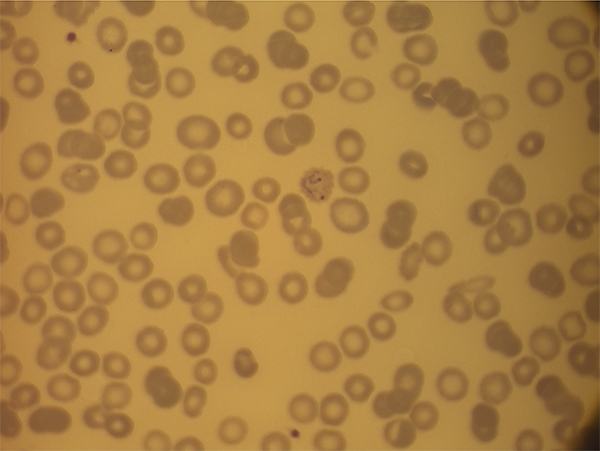
\includegraphics[width=3.5cm]{images/malaria/f1a}
	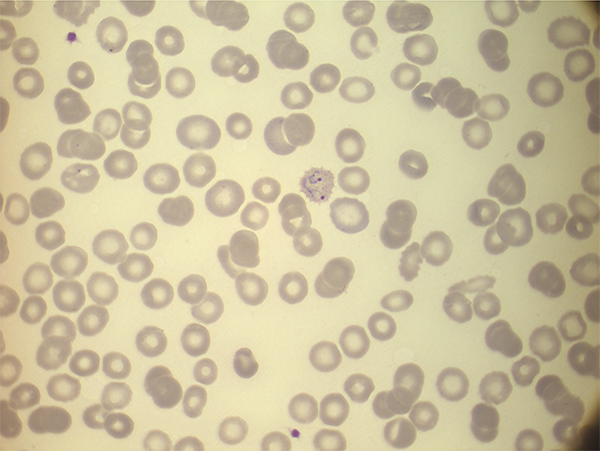
\includegraphics[width=3.5cm]{images/malaria/f1b}
	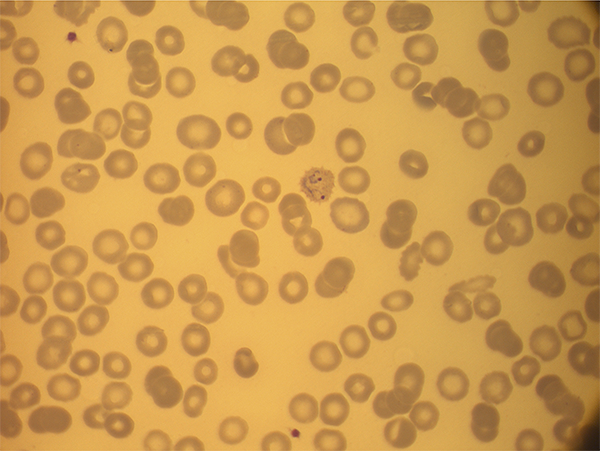
\includegraphics[width=3.5cm]{images/malaria/f1c}
	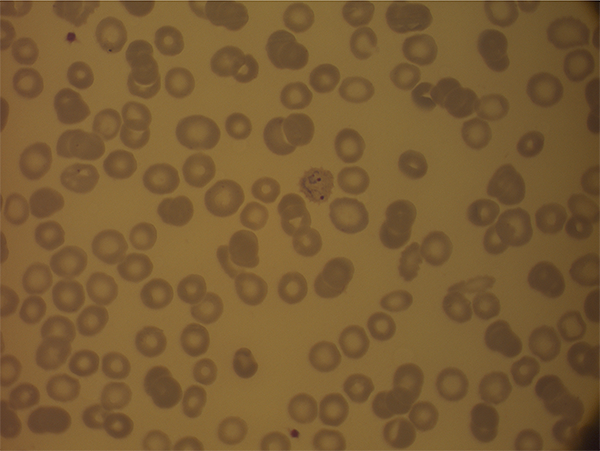
\includegraphics[width=3.5cm]{images/malaria/f1d}
	\caption{\label{fig:images_types} Different illumination conditions generate different images because of the absence of a standardized acquisition procedure. From left to right: acquisition of the same smear with four microscope's brightness levels. Courtesy of CHUV, Lausanne.}
	
\end{figure}

\section{Peripheral Blood Images}
There are several components in blood smears containing peripheral blood samples. Consequently, peripheral blood images usually consists of, at least, three main objects of interest: the White Blood Cells (\acs{WBC}s), the Red Blood Cells (\acs{RBC}s) and the platelets (or thrombocytes). 

\begin{figure}[!htbp]
\centering
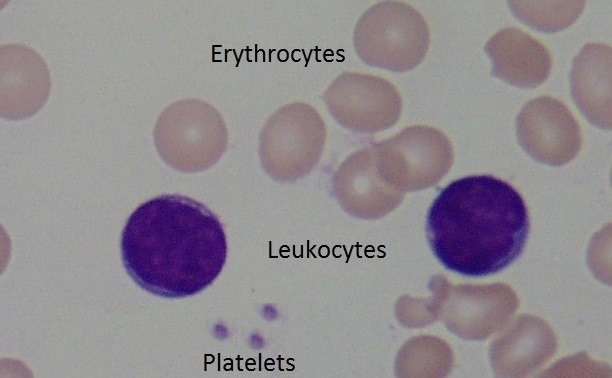
\includegraphics[height=0.21\textheight]{images/Cells1}
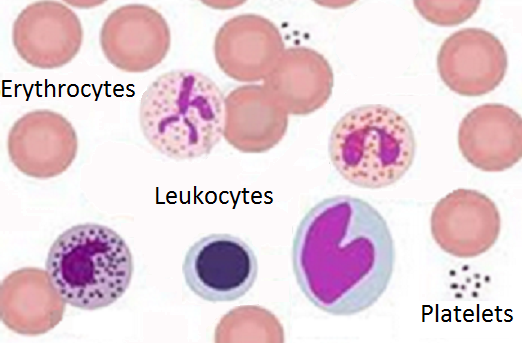
\includegraphics[height=0.21\textheight]{images/Cells2}
\caption{\label{fig:leukocytes} Peripheral blood smear components: a real image and a schematic representation.}
\end{figure}

Platelets or thrombocytes are small non-nucleated disc shaped cells with a diameter between 1 and 3 $\mu$m. Upon release into the peripheral blood from the bone marrow, they appear as fragments. They play a major role in haemostasis leading to the formation of blood clots when there is blood vessel injury or other bleeding, starting to clump together to form aggregates. There must be a sufficient number of platelets to control bleeding. If too few are present, or if they do not work properly, the ability to form a clot becomes impaired and can be a life-threatening situation \cite{Ciesla}. Normal, mature RBCs or erythrocytes are uniform in size, 7-8 $\mu$m in diameter,  and do not have a nucleus as most other cells do. They are round and flattened like a donut with a depression in the middle instead of a hole (biconcave). Due to the haemoglobin inside the RBCs, they appear pink to red in colour with a pale centre once the staining process has been completed. Considering that not every RBC could respect its typical shape, any significant number of cells that are different in shape or size may indicate the presence of some diseases \cite{Erhabor}. WBCs or leukocytes have a nucleus surrounded by cytoplasm, instead. This is one particular reason that let them be easily identifiable, as their nucleus appears darker than the background. However, the analysis and the processing of data related to the WBCs are complicated due to wide variations in cell shape, dimensions and edges. The generic term leukocyte refers to a set of cells that are quite different from each other. Indeed, although they are all derived from bone marrow stem cells, in the bone marrow, they differentiate themselves into two main groups: cells containing granules, called granulocytic or myelocitic, and cells without granules called mononuclear or lymphoid. Thus, we can distinguish between these cells according to their shape or size, the presence of granules in the cytoplasm and the number of lobes in the nucleus, as it can be seen in Fig.~\ref{fig:leukocytes}. The lobes are the most substantial part of the nucleus, and thin filaments connect them to each other. WBCs mature into five distinct cells types, that include neutrophils, basophils and eosinophils in the granulocytic group and lymphocytes and monocytes in the non-granulocytic group. Neutrophils are certainly the most common WBCs in a healthy adult, present in the human blood at a percentage ranging between 50 and 70\%. They range in size from 10-15 $\mu$m, and present a cytoplasm with pink or purple granules. They are distinguishable also due to the number of lobes present in the nucleus, which can range from 1 to 6 according to the cell maturation. They are involved in the defence against infections. Basophils are the least common of the granulocytes and represent only 0-1\% of all leukocytes in human blood. They have a diameter of approximately 10 $\mu$m. Generally, basophils have an irregular, plurilobated nucleus that is obscured by large and dark granules. Eosinophils are easily recognized in stained smears due to the presence of large, red-orange granules, which include para-crystalline structures in the shape of a coffee bean. They are round, 10-12 $\mu$m in size, and have a nucleus with two lobes. Generally low in number, present at 1-5\% in human blood, they most often increase in number in individuals with allergies and parasitic infections. Monocytes are usually the most voluminous WBCs, with a diameter of 12-20 $\mu$m and are often referred to as scavenger cells (phagocytes). They can ingest particles such as cellular debris, bacteria, or other insoluble particles. They represent 3-9\% of circulating leukocytes. Their nucleus is large and curved, often in the shape of a kidney. Lymphocytes are usually the smaller WBCs, with a diameter of 7-12 $\mu$m. They are characterised as having a smooth, round nucleus and a small amount of cytoplasm and often a smooth chromatin pattern. They are very common in human blood, with a percentage of 20-45\%. 

\begin{figure}[!htbp]
\centering
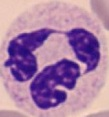
\includegraphics[height=0.125\textheight]{images/crop-Fig2-1}
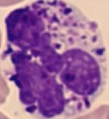
\includegraphics[height=0.125\textheight]{images/crop-Fig2-2}
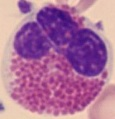
\includegraphics[height=0.125\textheight]{images/crop-Fig2-3}
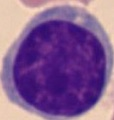
\includegraphics[height=0.125\textheight]{images/crop-Fig2-4}
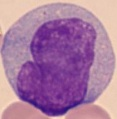
\includegraphics[height=0.125\textheight]{images/crop-Fig2-5}
\caption{\label{fig:leukocytes}A comparison between different types of WBCs: neutrophils, basophils, eosinophils, monocytes and lymphocytes.}
\end{figure}

Numerous diseases and conditions can affect the absolute or relative number of WBCs and their appearance on a blood smear. More details of the conditions that affect the number and the morphology of kind of cells are listed in Appendix A. Examples of the most common diseases that involve variation in shape and number of blood cells include anaemia, haemophilia, general blood clots and bleeding disorders while more serious cases that need to be diagnosed are leukaemia, myeloma, and lymphoma. This thesis focused on the analysis of Acute Lymphoblastic Leukemia (ALL) and malaria.

\section{ALL - Acute Lymphoblastic Leukaemia}
Leukaemia is a blood cancer that can be detected through the analysis of WBCs. There are two types of leukaemia: acute and chronic. According to the French-American-British (FAB) classification model \cite{Bennett}, acute leukaemia is classified into two subtypes: acute lymphoblastic leukaemia (\acs{ALL}) and acute myeloid leukaemia (AML). Here, only ALL has been considered, which affects a group of leukocytes called lymphocytes. ALL primarily affects children and adults over 50 years of age. The risk of developing ALL is highest in children younger than 5 years of age, and it declines and begins to rise again after age 50. Due to its rapid expansion into the bloodstream and vital organs, ALL can be fatal if left untreated \cite{Biondi}. Therefore, early diagnosis of this disease is crucial for a patients' recovery, especially for children. Diagnosis of ALL is based on the morphological identification of lymphocytes suffering from ALL, called lymphoblasts, by microscopy and the immunophenotypic assessment of lineage commitment and developmental stage \cite{Inaba}. Lymphoblasts present morphological changes that increment with increasing severity of the disease. In particular, lymphocytes are regularly shaped and have a compact nucleus with regular and continuous edges, whereas lymphoblasts are irregularly shaped and contain small cavities in the cytoplasm, termed vacuoles, and spherical particles within the nucleus, termed nucleoli \cite{Donida} (Fig.~\ref{fig:ex2}).

\begin{figure}[!t]
\centering
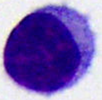
\includegraphics[height=0.125\textheight]{images/crop-BlastNo}
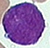
\includegraphics[height=0.125\textheight]{images/crop-BlastL1}
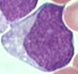
\includegraphics[height=0.125\textheight]{images/crop-BlastL2}
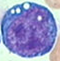
\includegraphics[height=0.125\textheight]{images/crop-BlastL3}
\caption{\label{fig:ex2}A comparison between lymphocytes suffering from ALL: a healthy lymphocyte, followed by lymphoblasts classified as L1, L2 and L3, respectively, according to the FAB \cite{Bennett}.}
\end{figure}

The observation of blood smears by skilled operators is one diagnostic procedure available to initially recognise the ALL, where the automatic counter fails due to the presence of abnormal cells. Human visual inspection is tedious, lengthy and repetitive, and it suffers from the presence of a non-standard precision because it depends on the operator's skill; these disadvantage limit its statistical reliability. The use of image processing techniques can help count the cells in human blood and at the same time to provide information about cell morphology, making them less expensive and providing more accurate standards. One of the goal of this thesis is to provide a fully automatic procedure based on the analysis of blood smear images, to support medical activity. This procedures counts the WBCs present in the smear through a process of segmentation and detection. The detected WBCs are then classified as suffering from ALL or not. 

\section {Related Works}
The progress of automated methods for the classification of blood cells from digitized images is a current problem in pattern recognition. These techniques can help to count the cells in human blood and, at the same time, be able to provide information on the morphological cells themselves. Unfortunately, for the analysis and processing of images, there are no standard techniques to apply to all types of images, but the processing must be adapted to the context. In particular regarding the blood smear images the processing techniques vary according to the type of blood cell to be analysed. In the literature, few attempts of automated systems, based on techniques of image processing, able to identify and classify peripheral blood cells have been proposed. Moreover, the existing systems are only partially automated, combining manual steps to automated ones. Furthermore, most of them do not work on the entire analysis process, but on individual phases of the whole analysis process. This section will show the techniques most commonly used by different authors at different stages of the process. 

The used methods of pre-processing depend on many variables, such as lighting conditions, the duration of the dye, defects caused by visual artefacts or not uniform background. The images should be processed in order to improve certain characteristics or to reduce further operations that could be required in the later stages of the analysis. The main issues addressed at this stage include noise reduction and enhancement of some structures of the images. Mohapatra et al. \cite{Mohapatra10a,Mohapatra10b,Mohapatra10c,Mohapatra14} used a median filter to remove the noise followed by a Unsharp filter. The median filter has been preferred to the average filter since it preserves details of edges and then are enhanced with the use of the Unsharp filter. Other authors instead to enhance the quality of the images preferred operations based on the histogram such as contrast stretching or the histogram equalisation in order to redistribute the grey level values. Often these two transformations have been used in combination between them or with other techniques, as the algorithm proposed in \cite{Madhloom} that starting from the grey scale image performs separately a contrast stretching and a histogram equalisation. Then a series of arithmetic operations between the two images just obtained is performed in order to highlight the nuclei of leukocytes. The results is very impressive because not only it
enhances the nuclei of leukocytes, but it drastically reduces the number of the other blood components, making the further steps much more simple.

As said previously in the analysis of medical images different levels of segmentation are used. In particular for what concerns peripheral blood images two main levels are used: the level of cells segmentation, which aims to separate whole cells from the background or plasma and the level of segmentation that tries to separate the various components inside the cell, such as the nucleus from the cytoplasm or intracellular parasites. Several authors have proposed methods for effective segmentation of the nucleus of leukocytes, while there are few attempts of segmentation of the cytoplasm. The characteristic generally used for segmentation is the intensity value of grey level images. However, many authors showed how the use of single channel from different colour spaces could be used to highlight differences between blood components. Indeed the nuclei of the white blood cells are more in contrast on the Green component of the RGB colour space \cite{Cseke}, while the cytoplasm of the white blood cells is more evident on the Hue component \cite{Wu} or the Saturation component \cite{Halim} of the HSV colour space. The Saturation component of the HSV colour space is also useful to identify and separate erythrocytes \cite{DiR} when present in complex agglomerates of cells, otherwise they can be easily detected and counted with a threshold value computed using Zack algorithm from grey level images \cite{Berge}. Based on this knowledge many algorithms of region growing have been proposed \cite{Kovalev, Lez98, Lez02} that use the pixels within the nuclei, identified previously, as seeds in order to segment the whole white blood cells. The cytoplasm is detected through iterative aggregation of the pixels surrounding the region of interest according to the homogeneity of the colours and the information of the gradient. Edge based segmentation methods are rarely used in this contest, since the boundaries between cells are not clearly defined. However, the performances of edge detection operations can be improved using morphological operators \cite{Piuri, Sco05} being able to connect in a better way the detected edges and restore the complete boundary of the cells. 

A further problem in the analysis of peripheral blood cell images is the presence of cells grouped together or adjacent, as showed in Fig. \ref{fig_clumps}. This is an important problem since it doesn't allow an analysis of the single cells, such as the computation of shape descriptors or the proportion of cytoplasm and nucleus. A priori knowledges about the average size and shape of the cells, allow to work on sub-images extracted from the original image, by cutting a square around the nucleus previously segmented \cite{Kovalev, Sinha}. Thus, assuming that each sub-image has only one white blood cell using some restrictions on the shape and the colour information it is possible to perform a clustering around the nucleus. Unfortunately this assumption is not always true, in fact it is possible to find more than one nucleus on a sub-image that affects the result of the clustering. An improvement of this approach works on the whole images without using the a priori knowledges about the size and shape. This is possible thanks to the distance transform \cite{Maurer} that associates to each pixel of the binary image its distance from the border. Thus, the maximum distance obtained can be used as a marker for a subsequent segmentation step \cite{Malpica}, or the distance image can be used directly as a shape delimiter for a watershed segmentation \cite{Lindblad}. The main drawbacks of these approaches is that the cells should be segmented perfectly since they work directly on the binary images. Furthermore, since the distance transform in this case works like a shape delimiter, it is able to separate only small agglomerates of cells that should have an almost circular shape.

\begin{figure}[h]
	\centering
	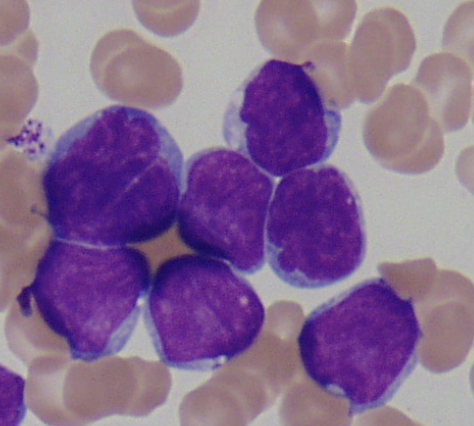
\includegraphics[height=0.25\textwidth]{images/2016_1_mva/clump}
	\caption{\label{fig_clumps}Crop of a sample image taken from ALL-IDB1. It represents a leukocyte clump.}
\end{figure}

The step of feature extraction is very important in the analysis of peripheral blood cells, as only with significant features, the system will be able to discriminate the various types of cells, the cells affected by diseases from the normal ones or the presence of other abnormalities in the blood. The idea is to extract the descriptors that best approach to the visual patterns indicated by pathologists. The colour and texture descriptors are certainly the most discriminatory features of blood cells. Generally this kind of images are acquired using the RGB colour space that allows a good discrimination of platelets, red blood cells and white blood cells, especially if the analysis is extended to all RGB channels \cite{Angulo}. However, the discrimination of subclasses of cells such as various types of leukocytes, usually requires the use of other colour spaces, taking into account all the colour channels or only the most discriminatory such as the H channel of the HSV colour space \cite{Hengen}. Furthermore, geometrical features can be used to discriminate cells with abnormal size or with irregular shape. Other geometrical features have been specifically proposed to classify the type of nucleated cells, since they can be distinguished not only using the ratio between cytoplasm and nucleus \cite{Piuri, Sco05, Sco06} but also extracting the number of lobes of the nucleus. Extract the number of lobes means count the more substantial parts of the nucleus connected by thin filaments. This is not an easy task, since the connection between the lobes sometimes can appear larger than normal and thus, also a skilled operator, could count two small lobes as it was only one. A good approximation of the number of lobes can be obtained by iterative erosion of the nucleus. The number of lobes correspond to the connected components with an area bigger than a prefixed parameter \cite{Piuri}.  

Once the features have been extracted they must be inserted in a process which classifies cells based on haematological concepts \cite{Biondi, Serbouti}. Different learning methods have been used to classify blood cells, but above all very different choices about the number of classes have been taken. The choice taken more frequently is the binary classification to distinguish healthy white blood cells from abnormal ones making use of the SVM classifier, which is excellent in the separation of binary classes with pattern very close in space \cite{Mohapatra10a, Mohapatra10b, Mohapatra10c, Mohapatra14}. Instead, when the number of classes is higher the most used classifier have been the Neural Networks, performing a separation into the five types of leukocytes \cite{Sco06} or performing a separation into 7 classes, lymphocytes, neutrophils, eosinophils, other (monocytes and basophils), lymphocytic leukaemia L1, lymphocytic leukaemia L2 and non-lymphocytic leukaemia \cite{Buavirat}. 

In the following chapter you will see the algorithms proposed to create a full automated system for peripheral blood images. For clarity each step of the whole process has been discussed separately following the order mentioned before and used for most of the methods presented in literature. Furthermore in order to make a comparison with the state-of-the-art, each step of the proposed method has been tested using the same dataset presented below.

\section{Datasets}
The main problem in the testing phase ​of an automated system is certainly the absence of many public datasets. In fact, many authors have tested their methods by using only a few samples of images or private databases not publicly available. This disadvantage does not allow a direct comparison with the results obtained by similar proposed systems and it limits the reproducibility of possible innovations. Among the public datasets of peripheral blood samples image we found useful for our purposes, there are the following:
\begin{itemize}
	\item ALL-IDB \cite{Donida}
	\item IUMS-IDB \cite{Sarrafzadeh}
	\item SMC-IDB \cite{Mohamed}
\end{itemize} 
Acute Lymphoblastic Leukaemia Image Database (\acs{ALL-IDB}), has been proposed by Donida Labati in \cite{Donida}. It is a public image dataset of peripheral blood samples of normal individuals and leukaemic patients and it contains the relative supervised classification and segmentation data. So, this dataset allows not only to assess the quality of the algorithms for cell counting but also to assess the ability to discriminate the white blood cells affected from leukaemia from healthy ones. The sample images have been collected by the experts of the M. Tettamanti Research Centre for childhood leukaemia and haematological diseases, Monza, Italy. The ALL-IDB database has two distinct versions. The first version the ALL-IDB1 contains full size original images that can be used both for testing segmentation capability of algorithms, as well as the classification systems and image preprocessing methods, while in the second version the ALL-IDB2 is a collection of cropped area of interest of normal and blast cells that belong to the ALL-IDB1 dataset, so it can be used only for testing the performances of classification systems.

\begin{figure}[!htbp]
\centering
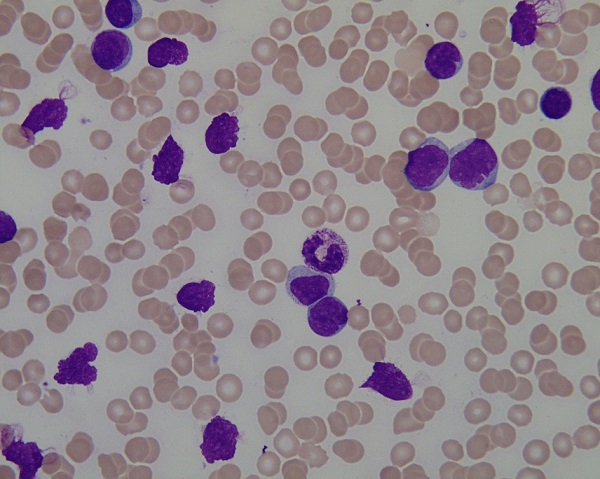
\includegraphics[height=0.25\textwidth]{images/Fig17-1}
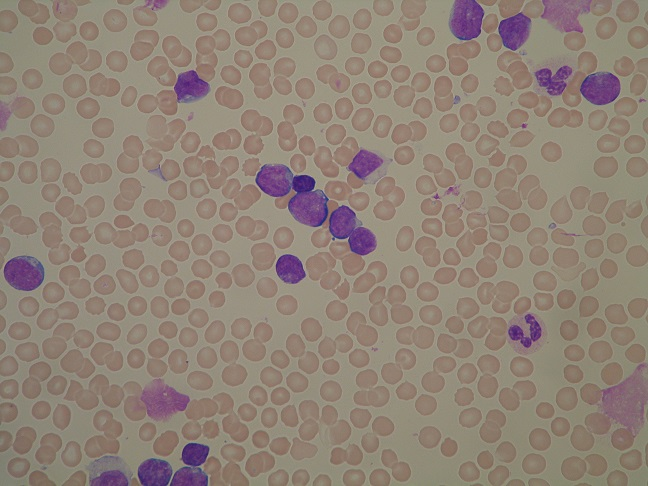
\includegraphics[height=0.25\textwidth]{images/Fig17-2}
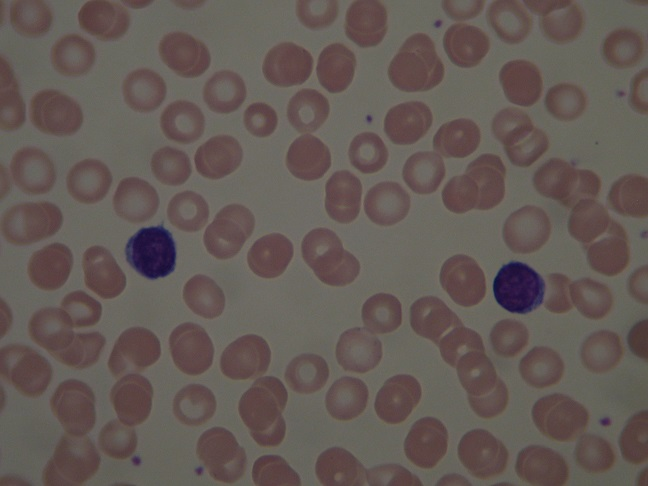
\includegraphics[height=0.25\textwidth]{images/Fig17-3}
\caption{\label{fig:dataset}Sample images from the ALL-IDB1}
\end{figure}

In both versions of the dataset, each image has an associated text file containing  the coordinates of the centroid of each candidate  lymphoblast, which was manually labelled by a skilled operator and can be used as a ground  truth for classification. The dataset ALL-IDB1 includes 108 images in JPG format with 24 bit colour depth. Most of the images in the dataset was captured with an optical laboratory microscope, with different magnifications ranging from 300 to 500, coupled with a Canon PowerShot G5 camera and their resolution is 2592x1944. The remaining images were acquired with a microscope at a constant magnification, coupled with an Olympus C2500L camera and their resolution is 1712x1368. Some images belonging to the ALL-IDB1 are showed in Fig.~\ref{fig:dataset}.

\begin{figure}[!htbp]
\centering
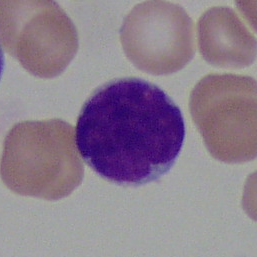
\includegraphics[height=0.16\textwidth]{images/Fig18-1}
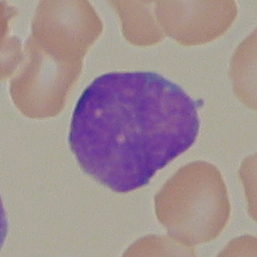
\includegraphics[height=0.16\textwidth]{images/Fig18-2}
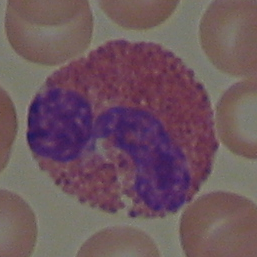
\includegraphics[height=0.16\textwidth]{images/Fig18-3}
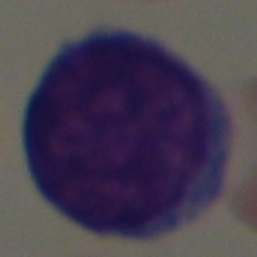
\includegraphics[height=0.16\textwidth]{images/Fig18-4}
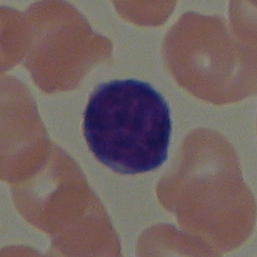
\includegraphics[height=0.16\textwidth]{images/Fig18-5}
\caption{\label{fig:dataset2}Sample images from the ALL-IDB2}
\end{figure}

As it can be seen from the sample images there are many differences both in terms of colour and illumination and both in terms of resolution and cells dimension. The dataset ALL-IDB2 includes 260 images in TIFF format with 24 bit colour depth. As said previously, these images are cropped areas of interest, containing a single leukocyte per image, belonging from the first version of the database. These images, differently from the first ones, have a standard size of 257x257, but being cropped area of them they present the same issues about colour, illumination and cells dimension, as it can be seen in Fig.~\ref{fig:dataset2}.

\begin{figure}[!htbp]
\centering
\hspace{-1.5mm}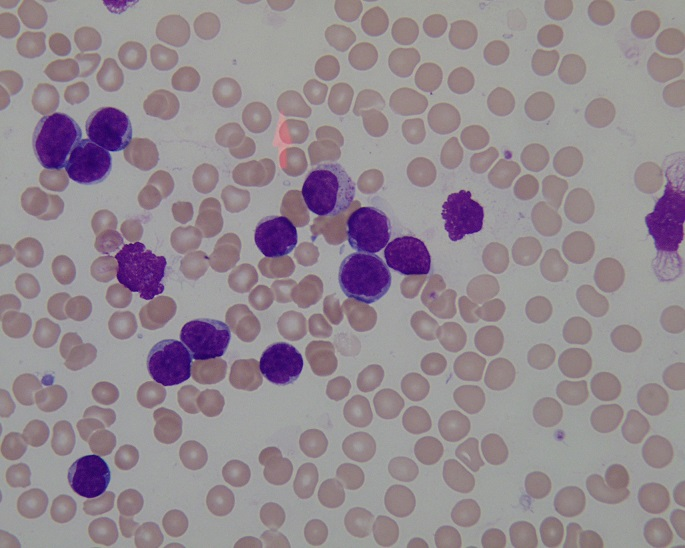
\includegraphics[width=0.24\textwidth]{images/Im003_1}\vspace{1 mm}
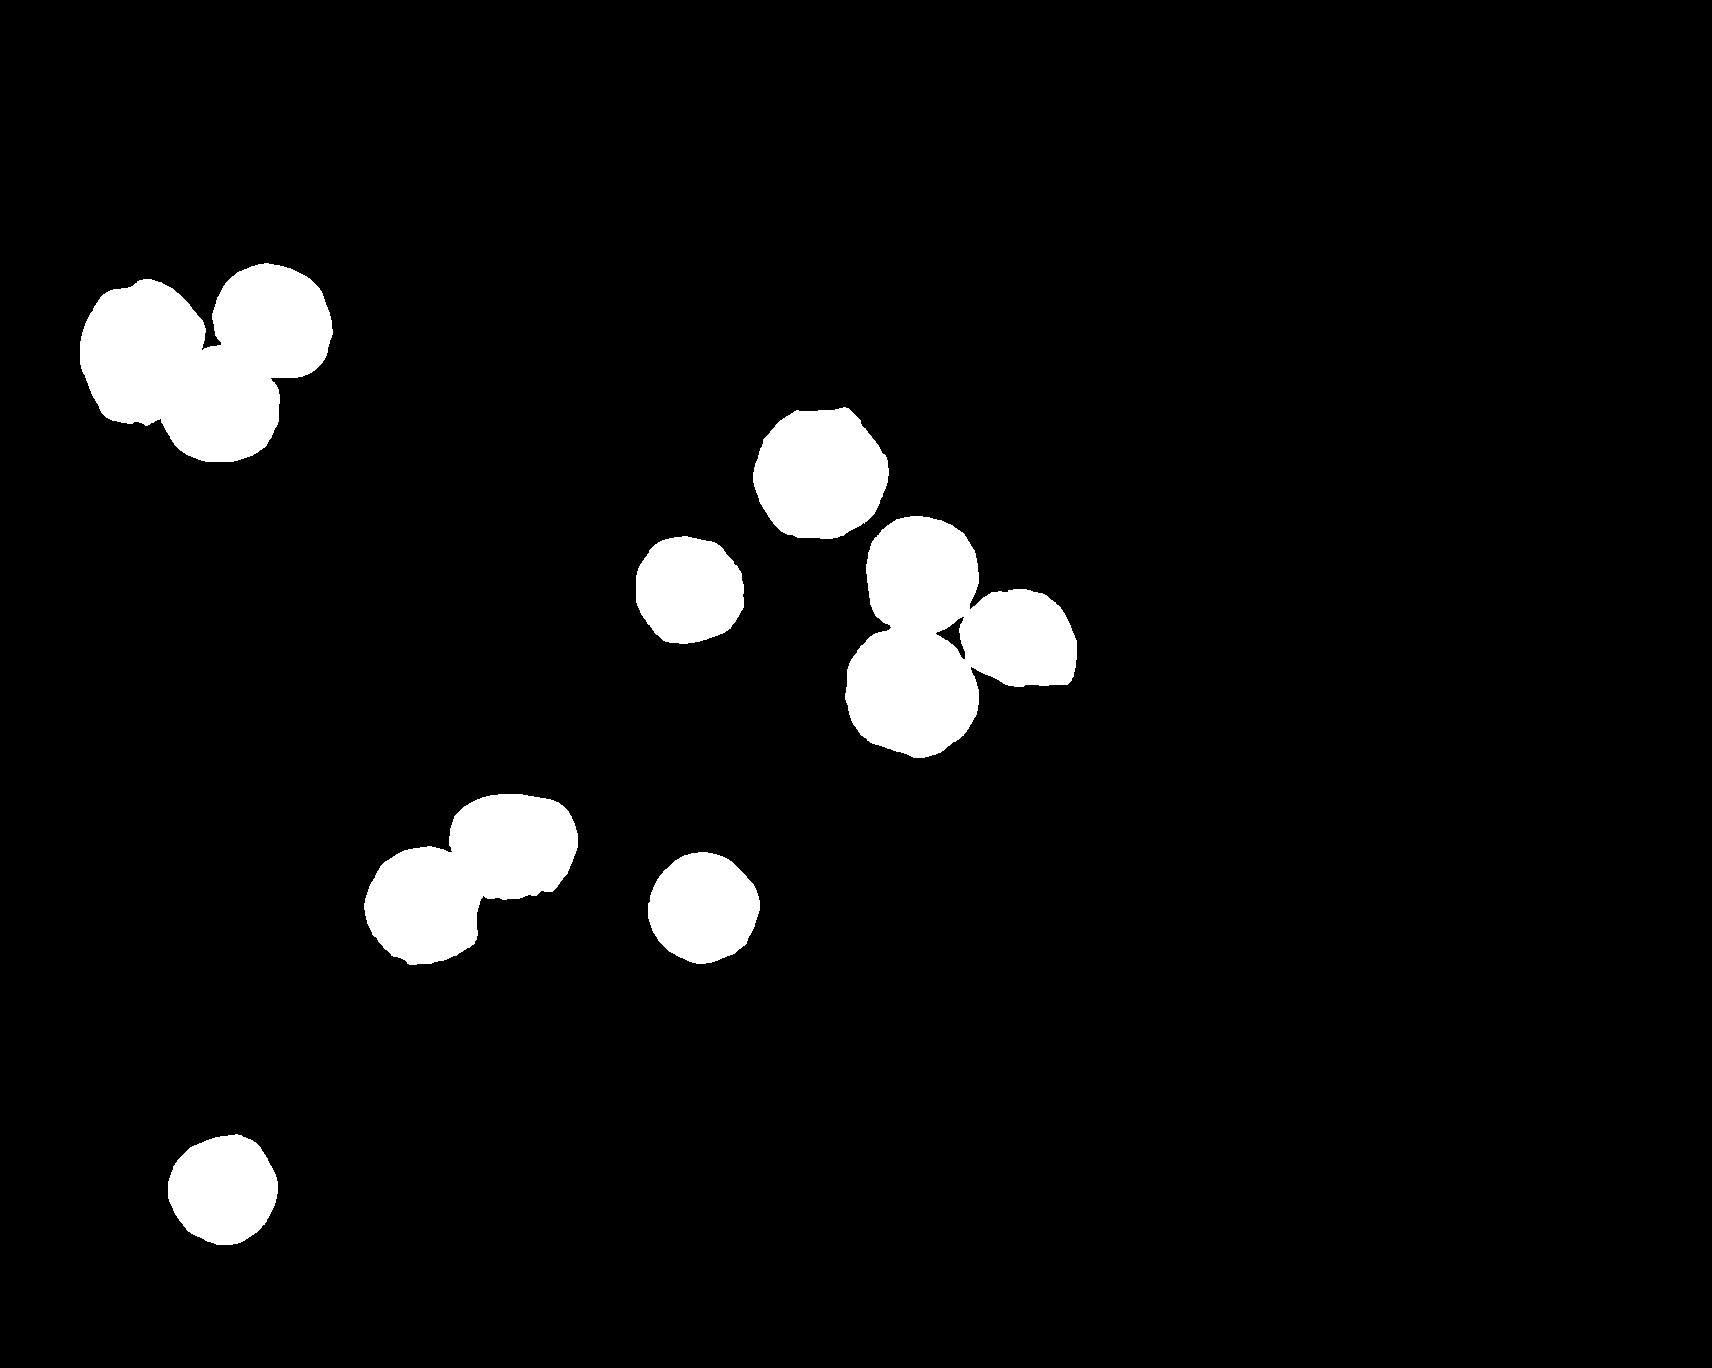
\includegraphics[width=0.24\textwidth]{images/Im003_1_WBC}
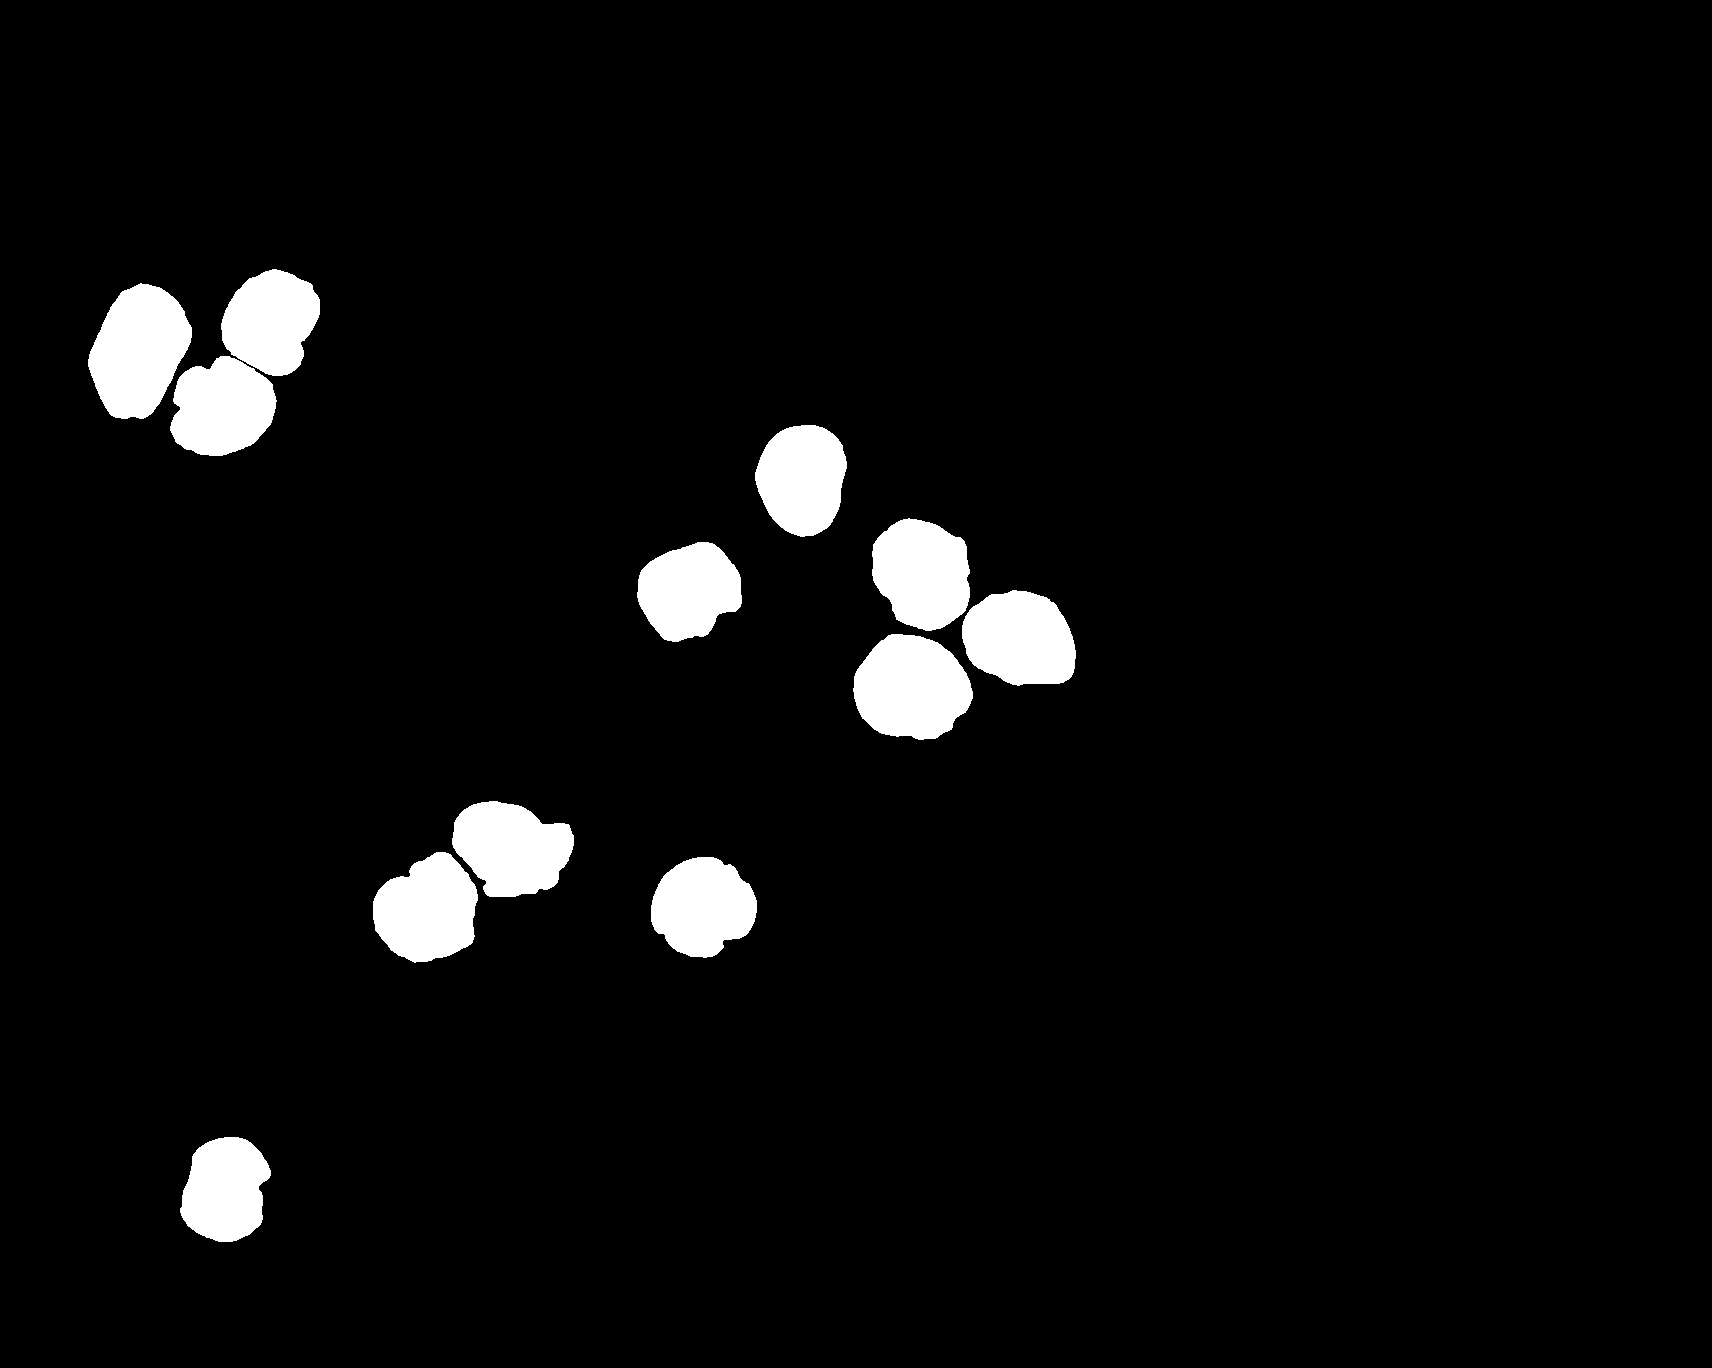
\includegraphics[width=0.24\textwidth]{images/Im003_1_WBCn}
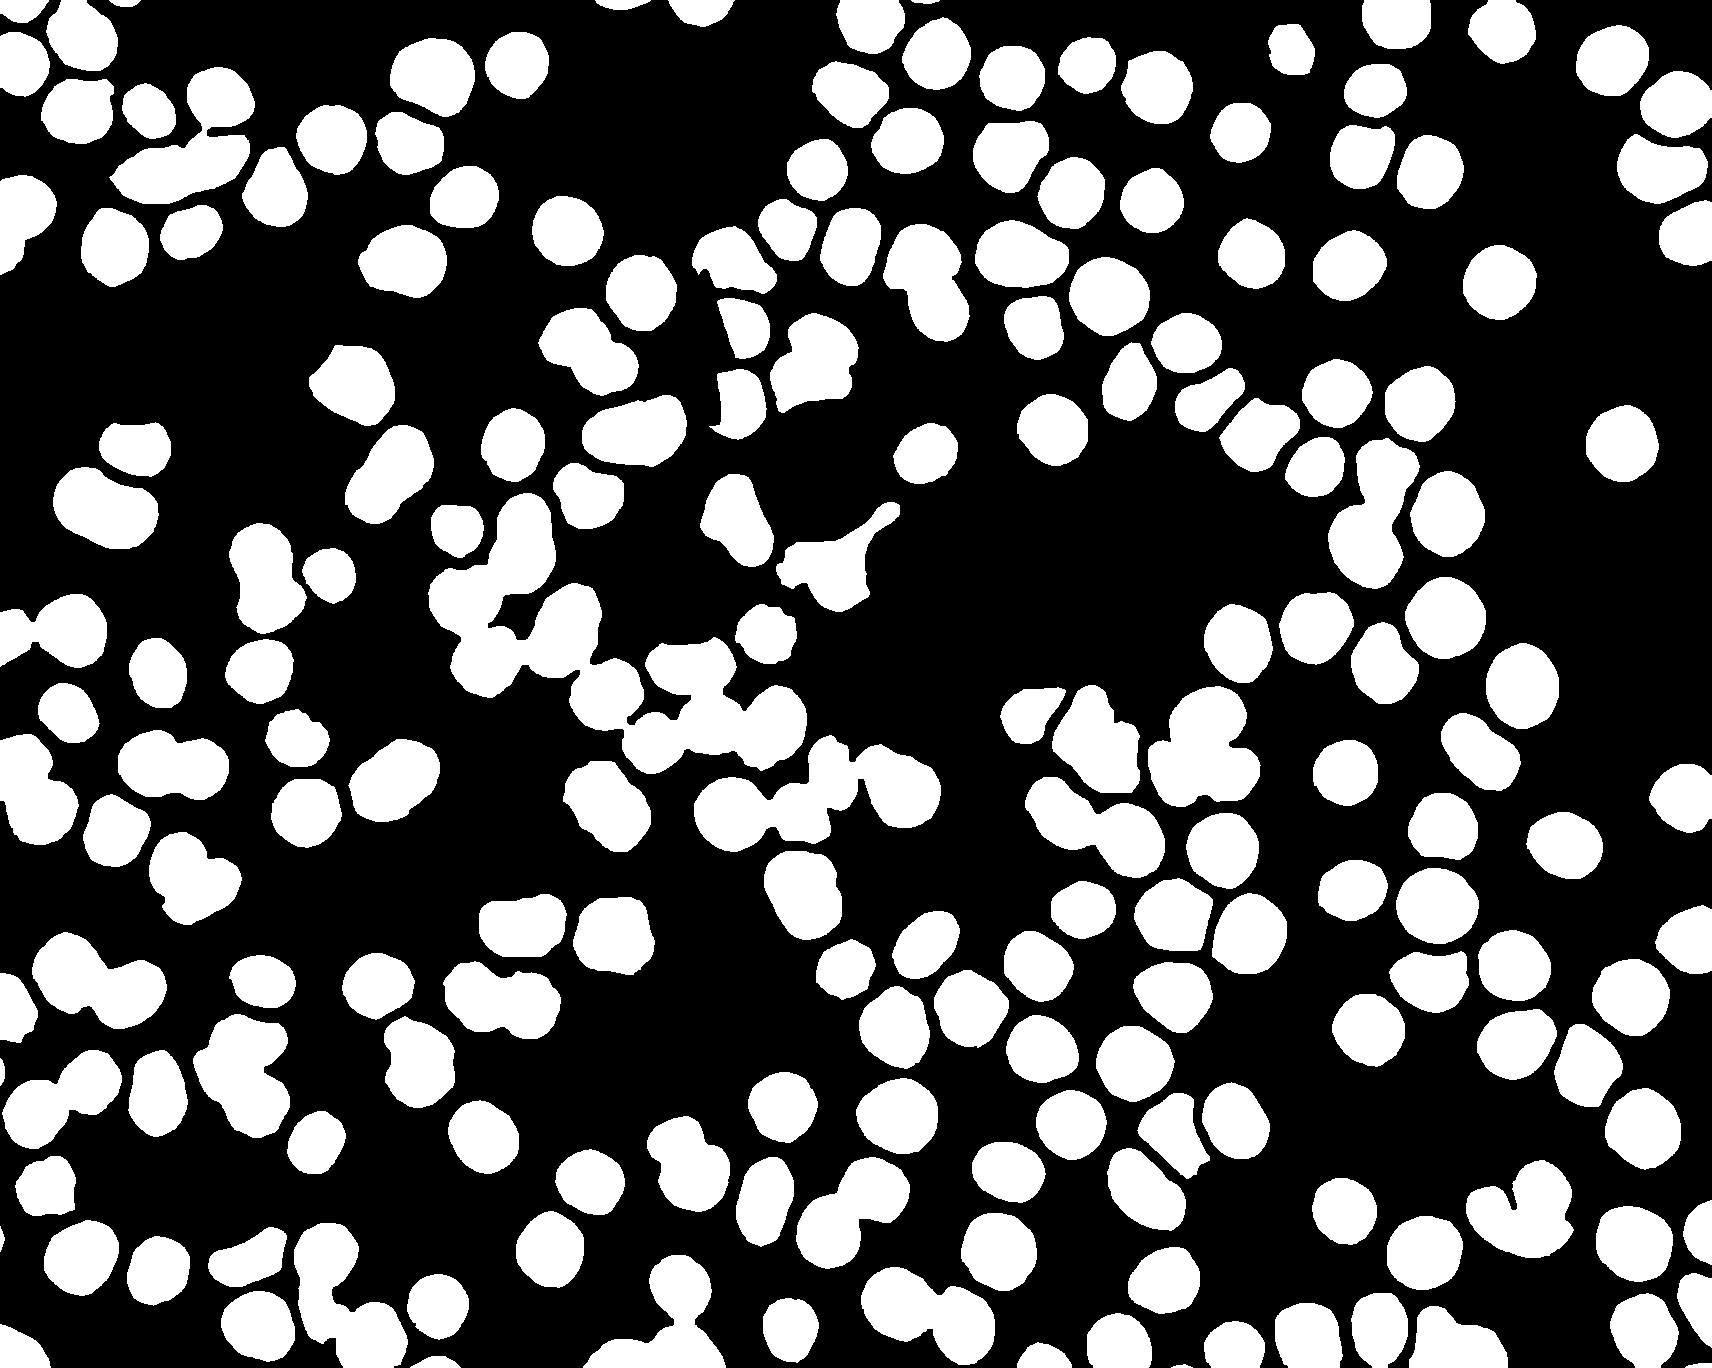
\includegraphics[width=0.24\textwidth]{images/Im003_1_RBC}
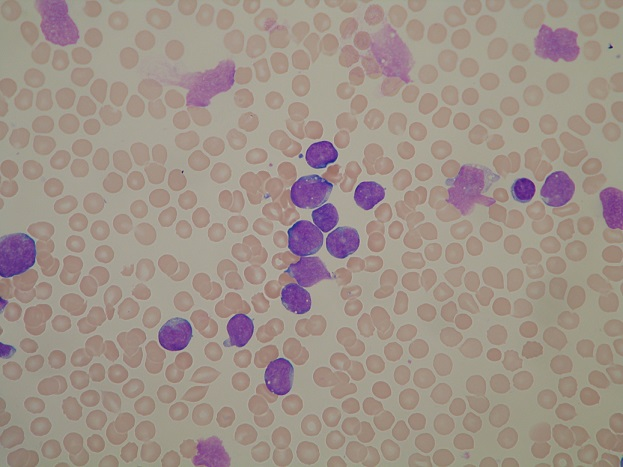
\includegraphics[width=0.24\textwidth]{images/Im050_1}
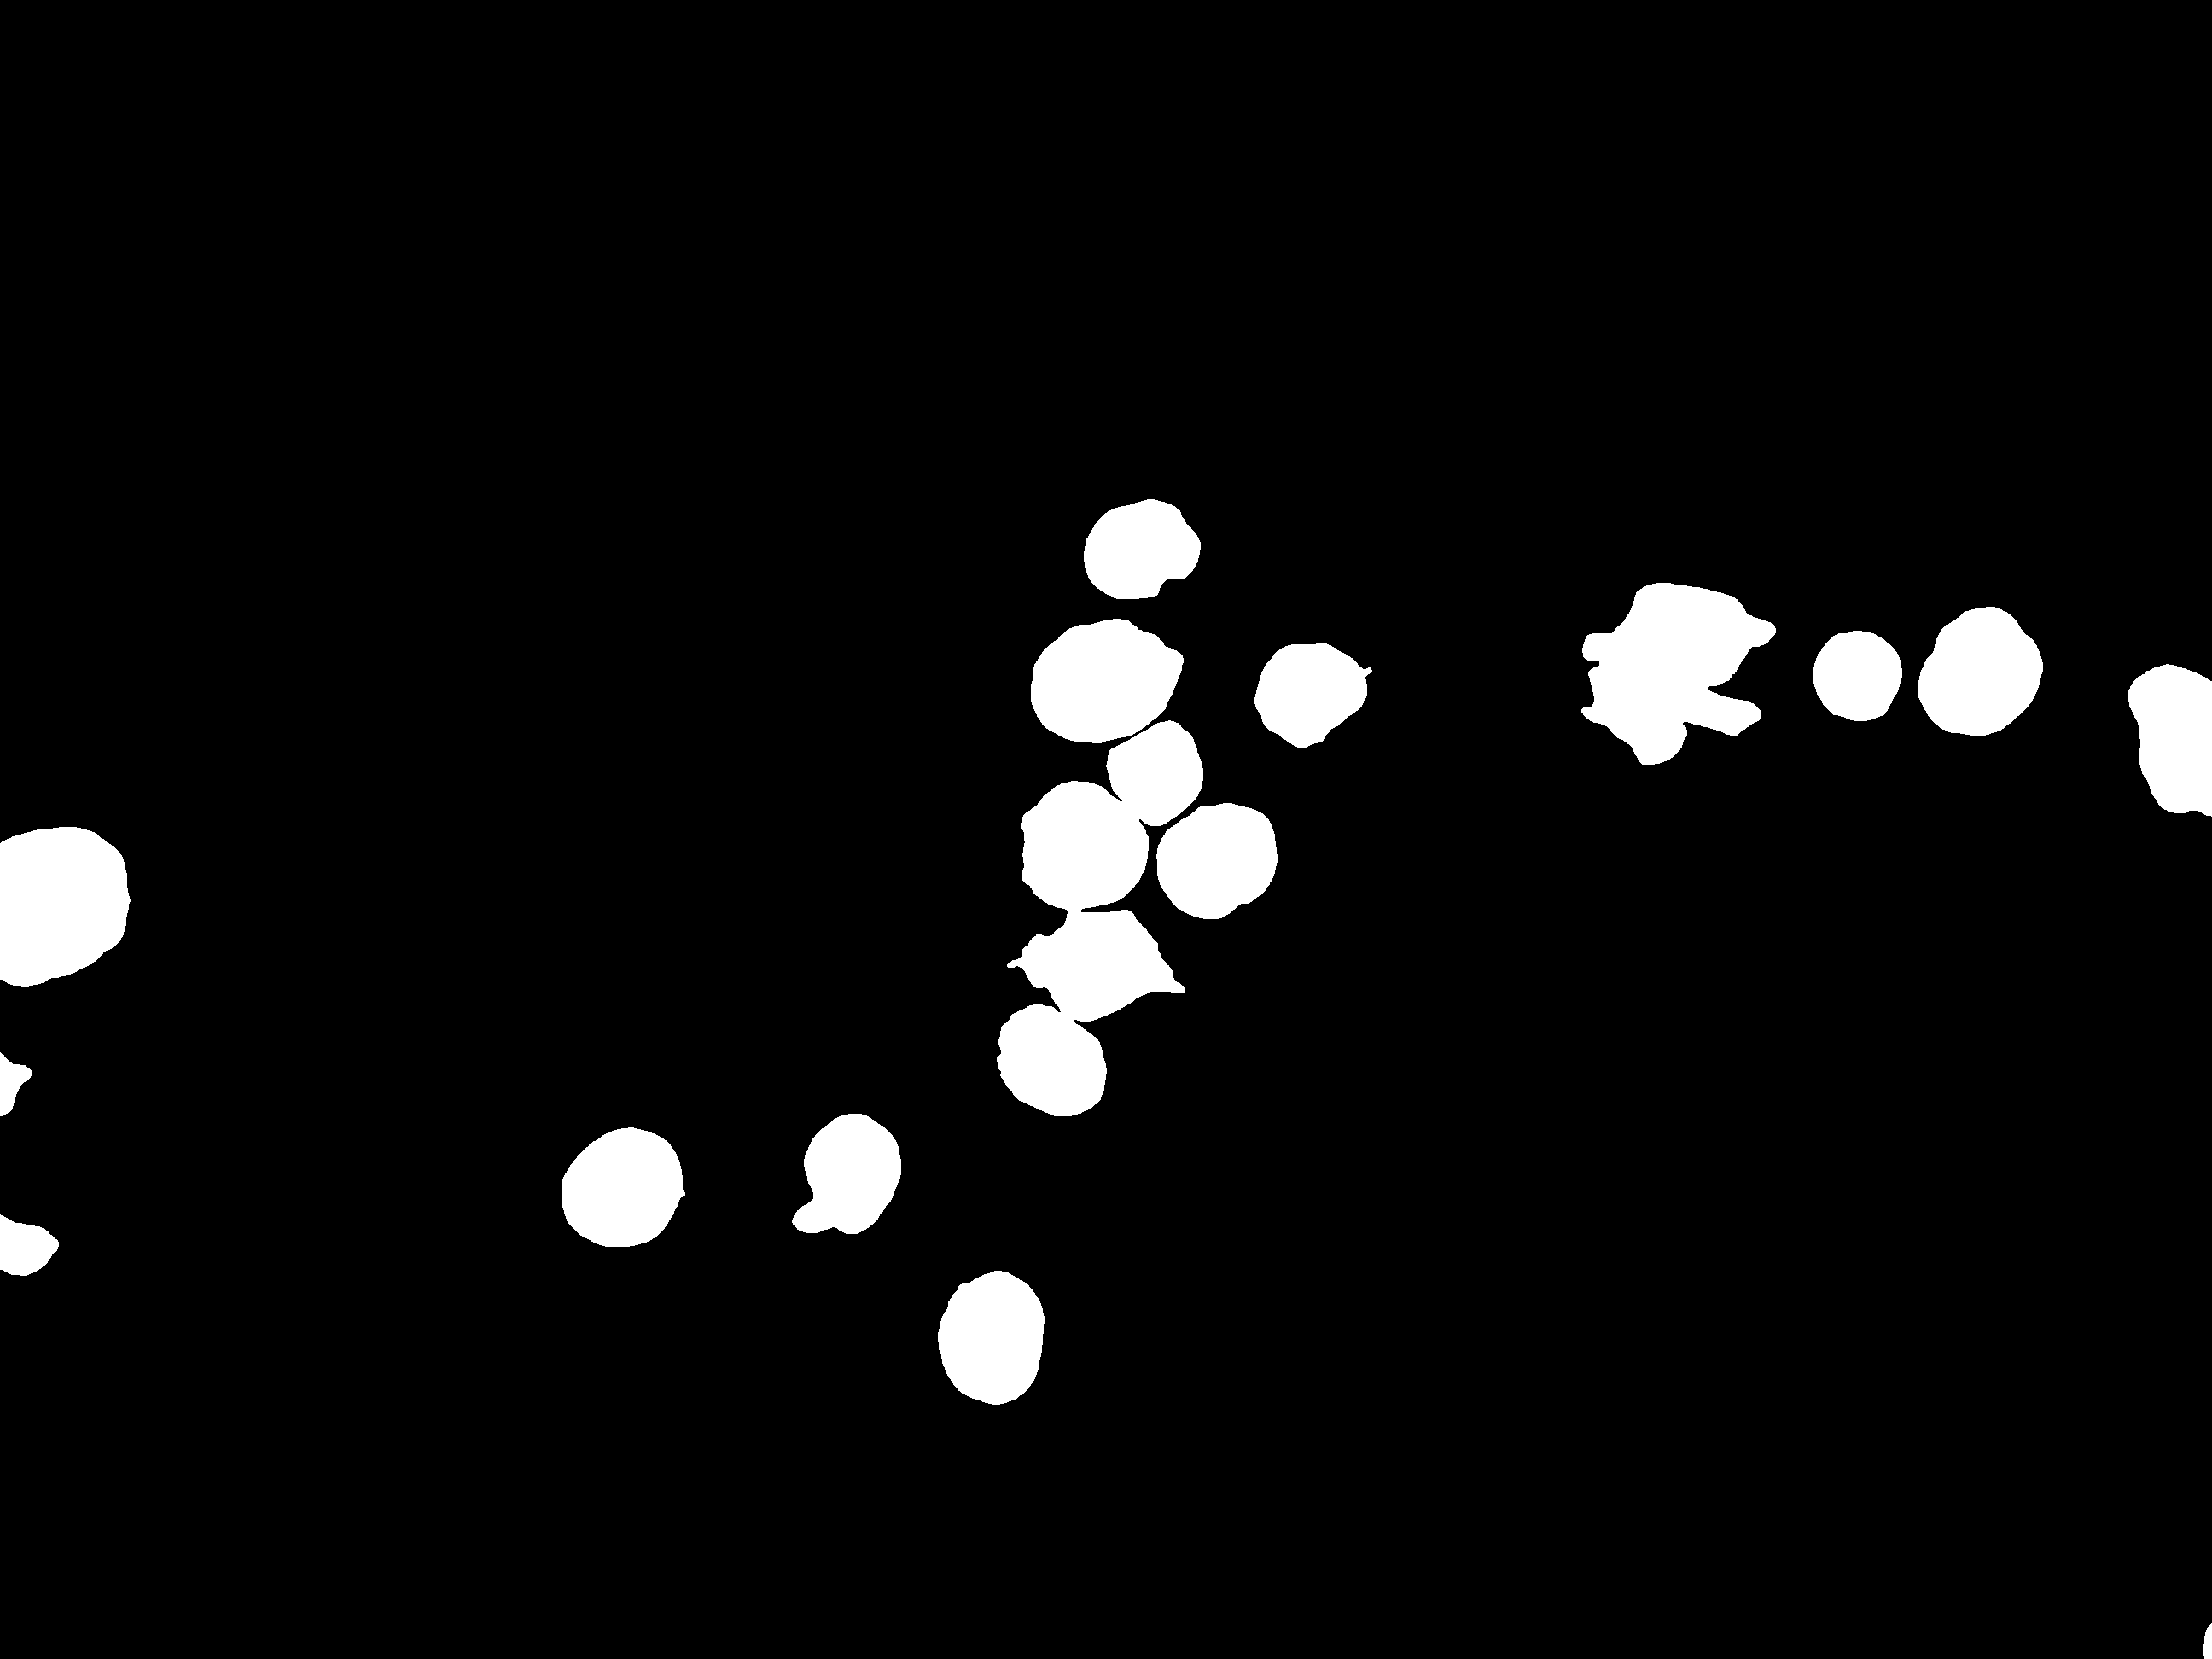
\includegraphics[width=0.24\textwidth]{images/Im050_1_WBC}
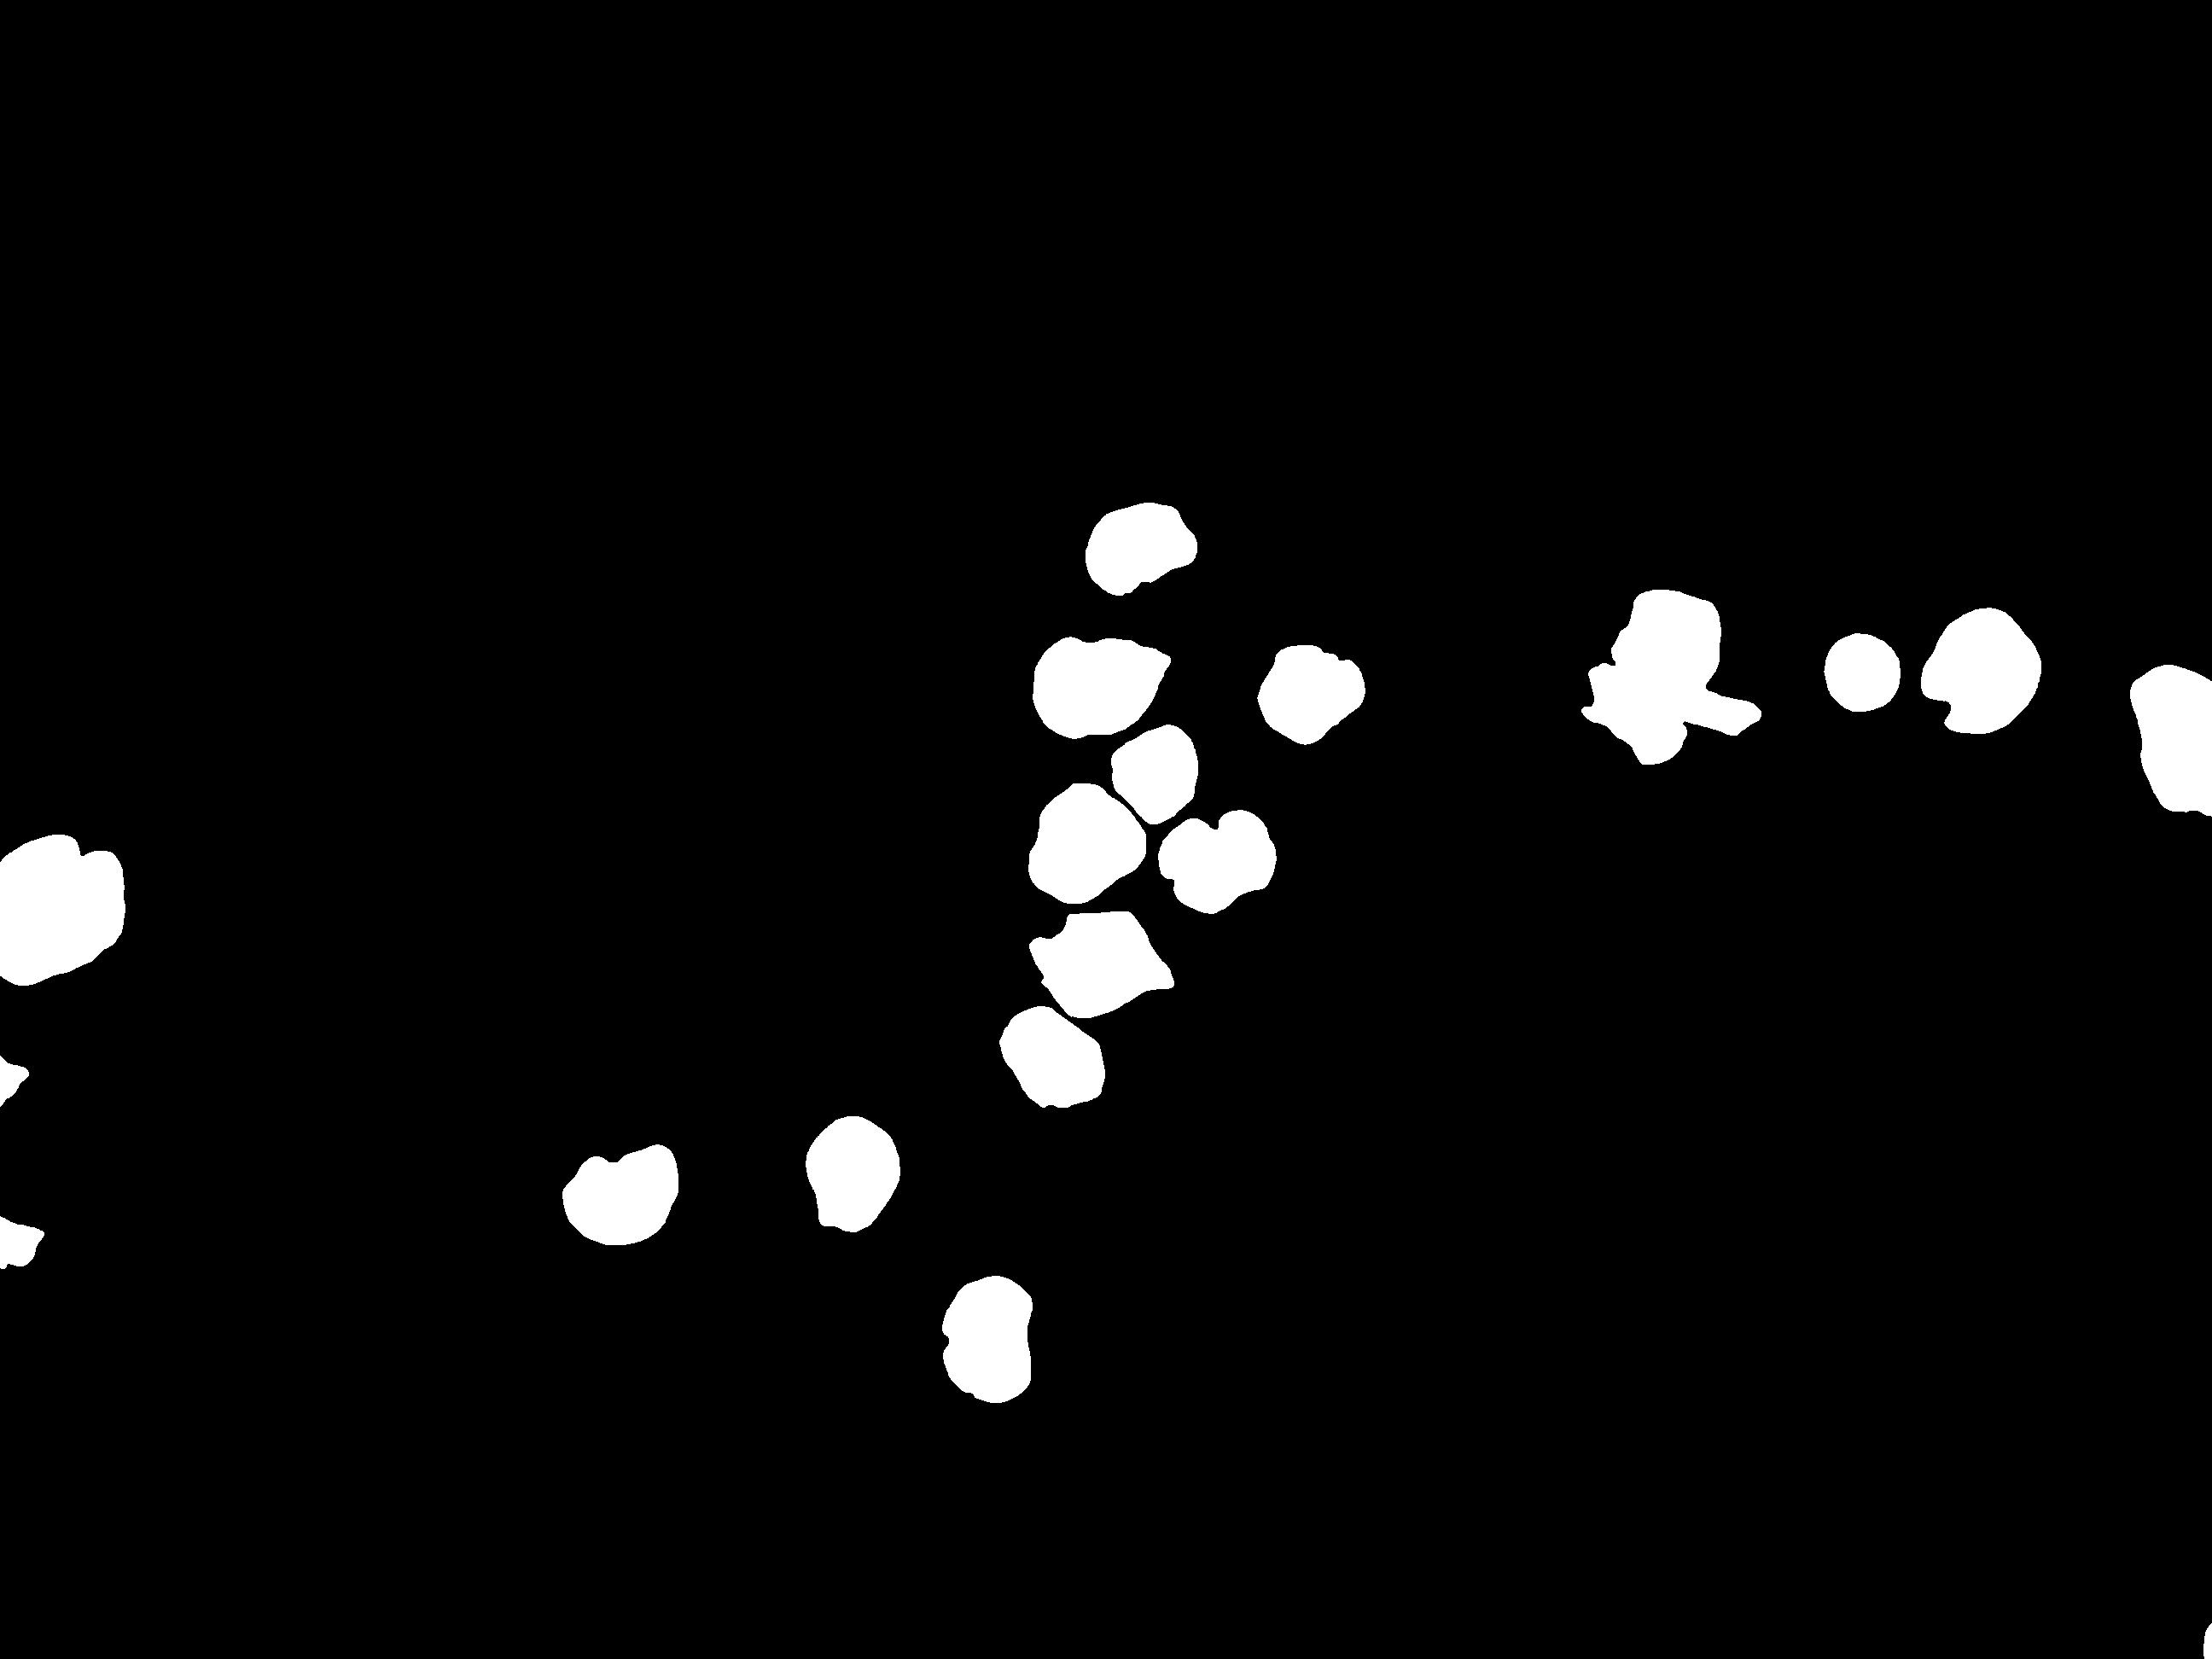
\includegraphics[width=0.24\textwidth]{images/Im050_1_WBCn}
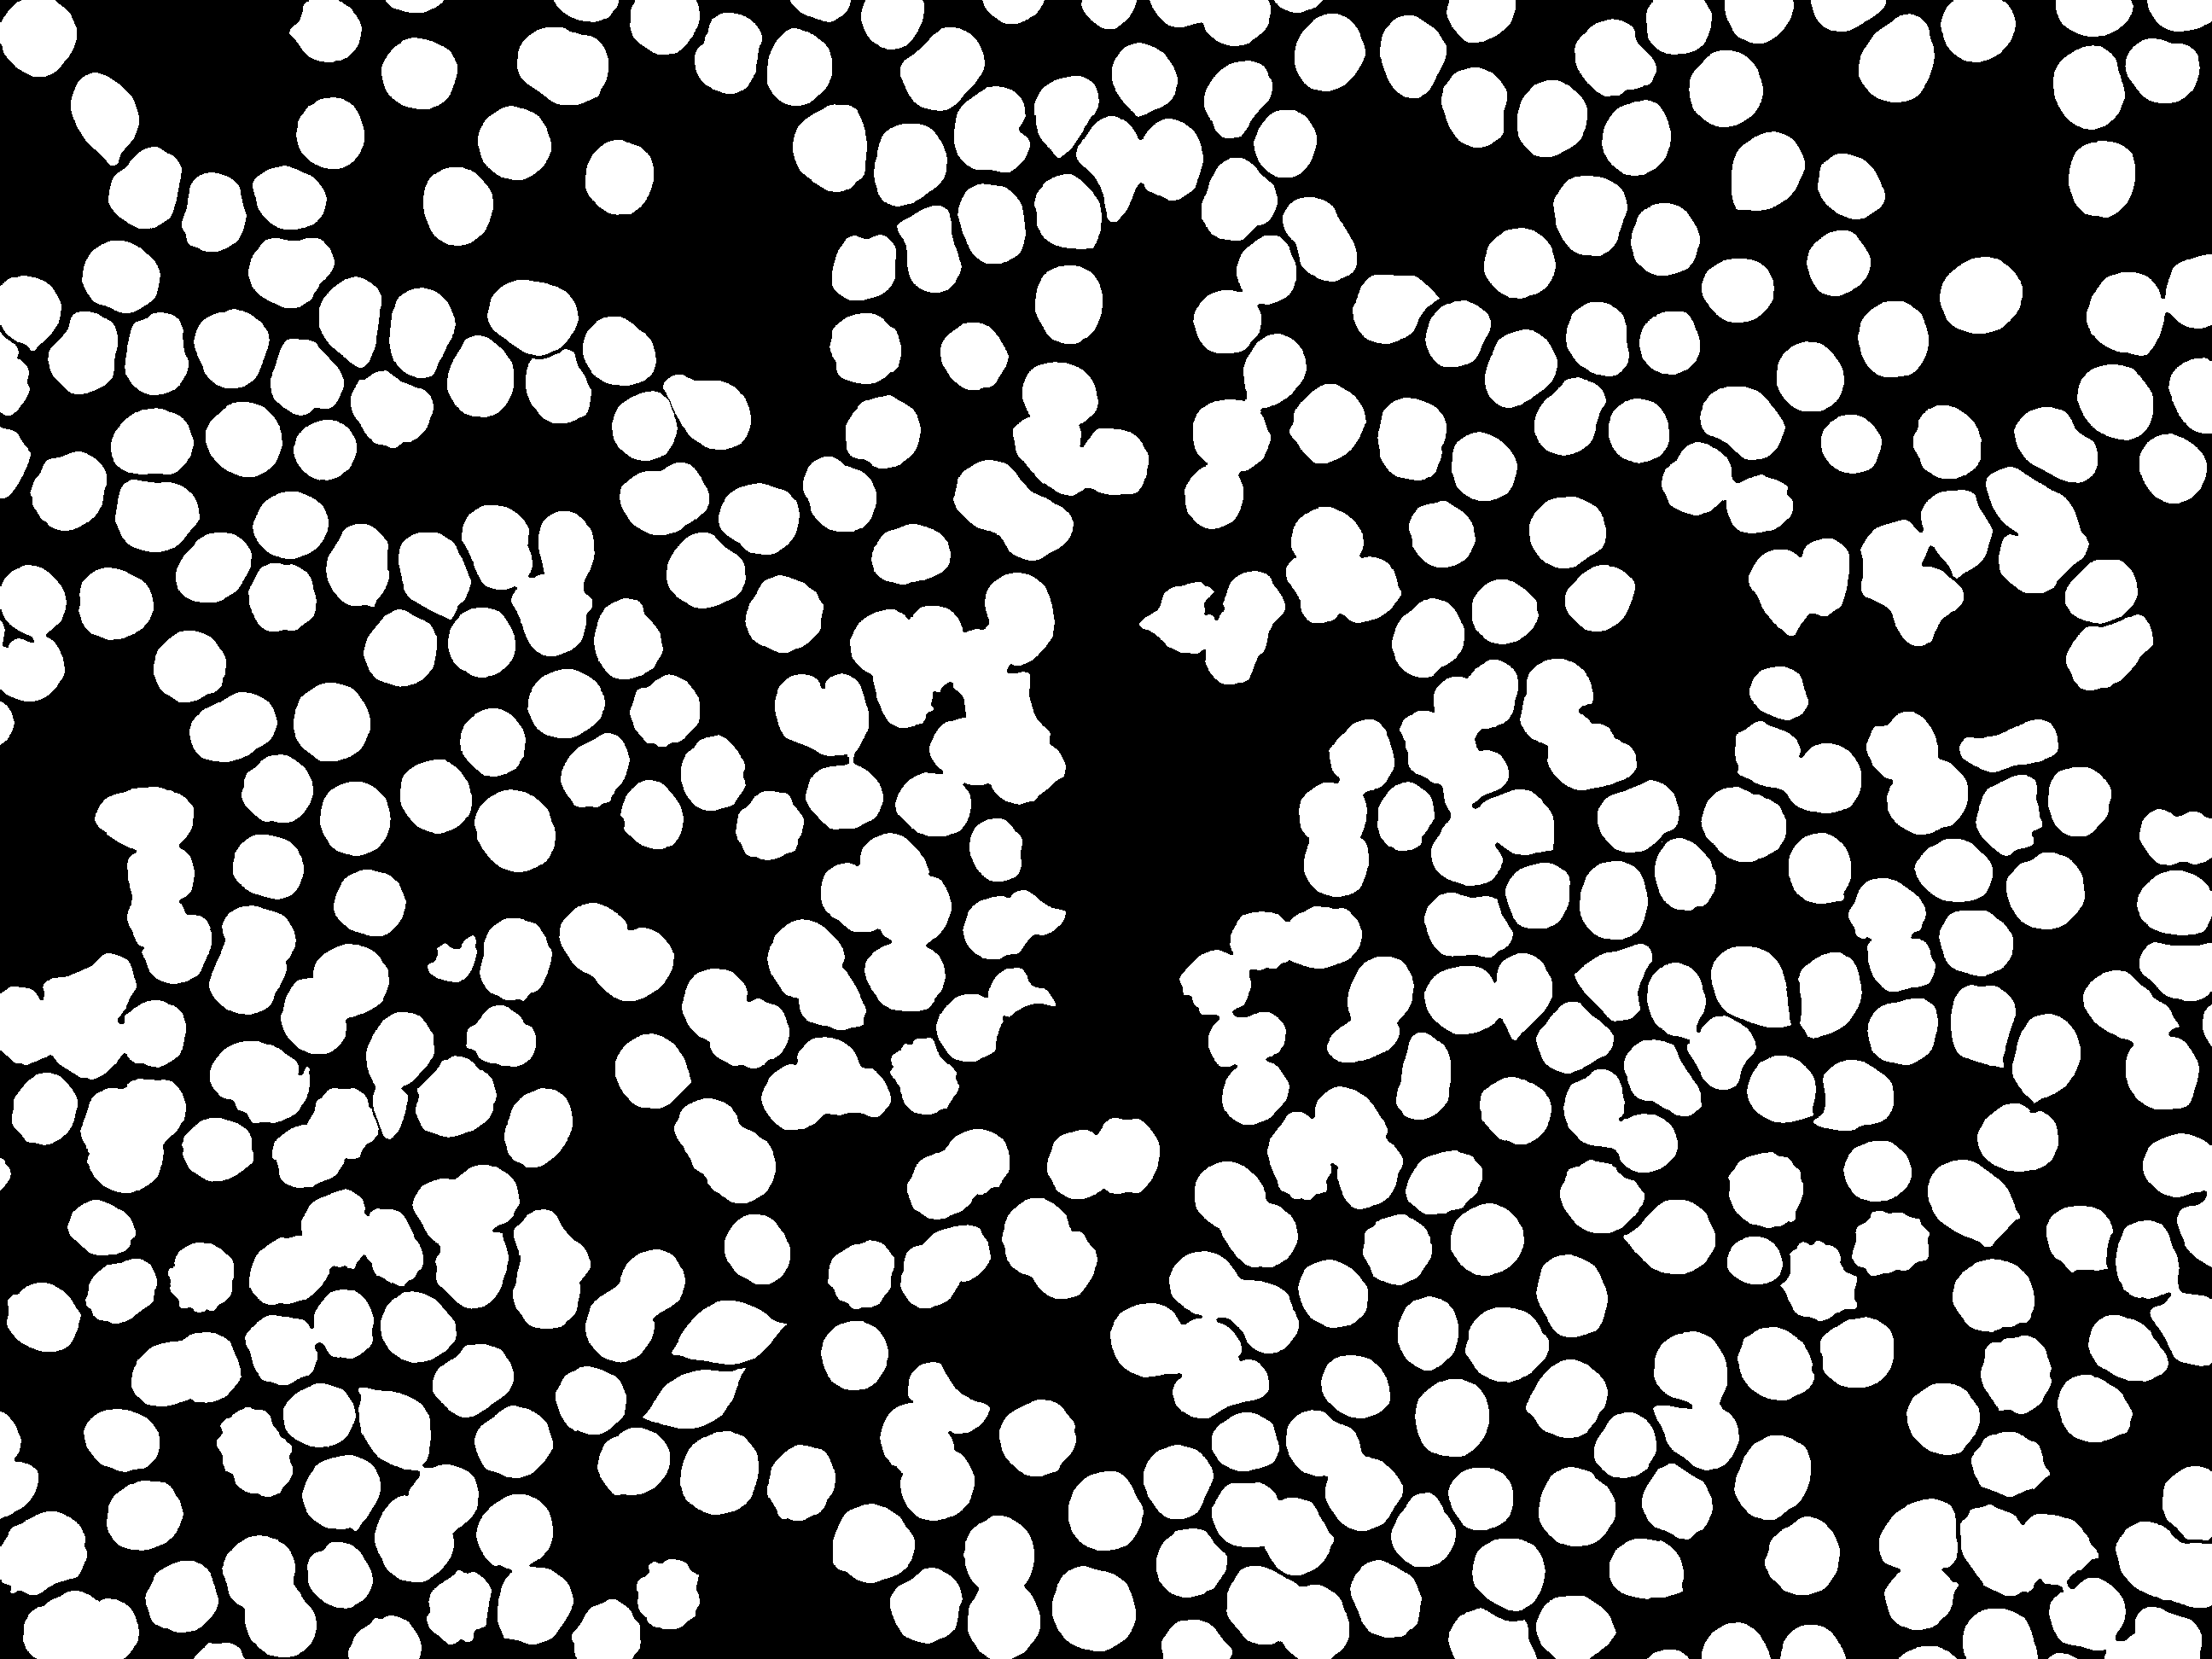
\includegraphics[width=0.24\textwidth]{images/Im050_1_RBC}
\caption{\label{fig:datasetgt1}From left to right: original images from the ALL-IDB1 database, ground-truth for whole leukocyte, only nuclei and RBCs}
\end{figure}

\begin{figure}[!htbp]
\centering
\hspace{12.5mm}
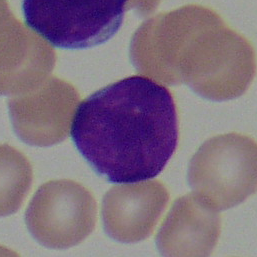
\includegraphics[width=0.16\textwidth]{images/Im035_1}

\includegraphics[width=0.16\textwidth]{images/Im035_1_WBC}\vspace{1 mm}

\includegraphics[width=0.16\textwidth]{images/Im035_1_WBCn}
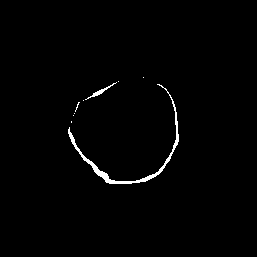
\includegraphics[width=0.16\textwidth]{images/Im035_1_WBCc} \hspace{15mm}
 
\hspace{15mm}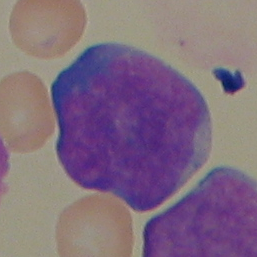
\includegraphics[width=0.16\textwidth]{images/Im091_1}

\includegraphics[width=0.16\textwidth]{images/Im091_1_WBC}

\includegraphics[width=0.16\textwidth]{images/Im091_1_WBCn}

\includegraphics[width=0.16\textwidth]{images/Im091_1_WBCc} \hspace{15mm}
\caption{\label{fig:datasetgt2}From left to right: original images from the ALL-IDB2 database, ground-truth for whole leukocyte, only nucleus and only cytoplasm}
\end{figure}

In order to evaluate the segmentation performances of the proposed method, a subset of 10 random samples images belonging to the ALL-IDB1 have been manually segmented by skilled operator, creating two ground-truth images for each sample. These images display respectively each blood cell present in the image and the white blood cell nuclei. Fig.~\ref{fig:datasetgt1} shows some images belonging to the ALL-IDB1 and their relative ground-truth images. Ground-truth images have also been extracted for images belonging to the ALL-IDB2, but in this case the manual segmentation is only devoted to the analysis of leukocytes, so the ground truth images display only the cytoplasm and the nucleus of the leukocyte, as it can be seen in Fig.~\ref{fig:datasetgt2}.
Despite our main efforts are devoted in designing a method able to achieve a robust segmentation with different image datasets, in our previous works \cite{Put15c,Put15d}  just the ALL-IDB dataset has been used, mainly because the proposed approach exploited the subdivision of the ALL-IDB dataset. Indeed, the ALL-IDB2 images were used to create the training set, being able to create a robust model to segment optimally the original images in ALL-IDB1. Our aim has always been to let our segmentation algorithm work for different kinds of images and, consequently, different datasets. 
For this reason, two more datasets have been used for testing the proposed method. 
IUMS-IDB is provided by the Iran University of Medical Science \cite{Sarrafzadeh}. It presents 100 microscopic images of size $732 \times 572$, taken from peripheral blood of 8 healthy subjects. These images are really different from the ones present in the ALL-IDB, since the microscope slides have been smeared and stained with a different staining technique. SMC-IDB, on the other hand, has been proposed in \cite{Mohamed}, presented at IEEE's 2012 SMC conference. It has been acquired from slides stained with the same staining technique as ALL-IDB. Nevertheless, the images are really different, since they have been acquired with a different combination of microscope and camera. This dataset provides a total of 367 peripheral blood images of size $640 \times 480$.
Sample images taken from IUMS-IDB and SMC-IDB are shown in \ref{fig:datasets_samples}.

\begin{figure}[h]
	\centering
	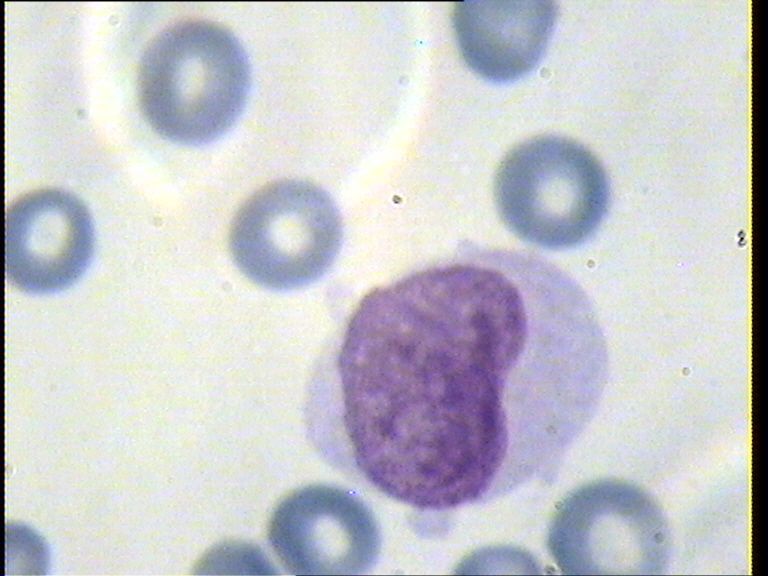
\includegraphics[height=0.33\textwidth]{images/2016_1_mva/IUMS}
	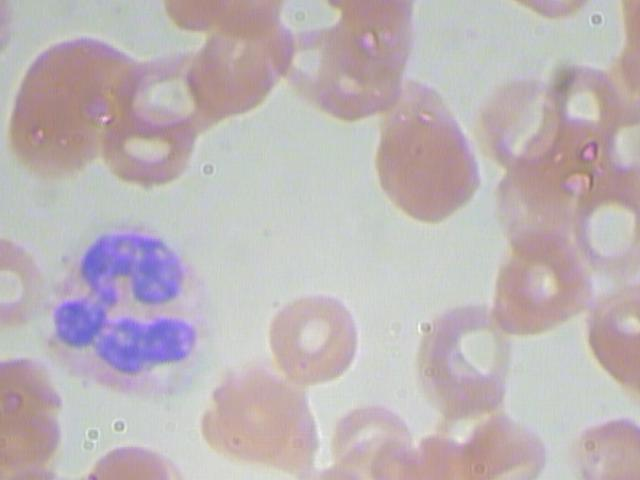
\includegraphics[height=0.33\textwidth]{images/2016_1_mva/SMC}
	\caption{\label{fig:datasets_samples}From left to right: sample image from IUMS-IDB and SMC-IDB.}
\end{figure}

\newpage
\section{Malaria}
Malaria is an epidemic health disease and a rapid, accurate diagnosis is necessary for proper intervention. 
Human malaria infection is not strongly related to cell count, but it needs different tests in order to be identified. It can only be caused by parasitic protozoans belonging to the \emph{Plasmodium} type. The parasites are spread to people through the bites of infected female Anopheles mosquitoes, called "malaria vectors".
There are five parasite species that cause malaria in humans and two of these species, \emph{Plasmodium falciparum} and \emph{Plasmodium vivax}, constitute the greatest threat. \emph{Plasmodium~ovale}, \emph{Plasmodium malariae} and \emph{Plasmodium knowlesi} are the three remaining species that are less dangerous in humans \cite{WHO_dec_2016}, as shown in Figure \ref{fig:malaria_types}.
All five species may appear in four different life-cycle stages during the infection phase in peripheral blood: ring, trophozoite, schizont and gametocyte. Some examples are shown in Figure \ref{fig:malaria_stages}.
The life-cycle-stage of the parasite is defined by its morphology, size and the presence or absence of malarial pigment.
The species differ in the changes of infected cell's shape, presence of some characteristic dots and the morphology of the parasite in some of the life-cycle-stages \cite{Somasekar2011}.

\begin{figure}[h]
	\centering
	\hspace{-1.5mm}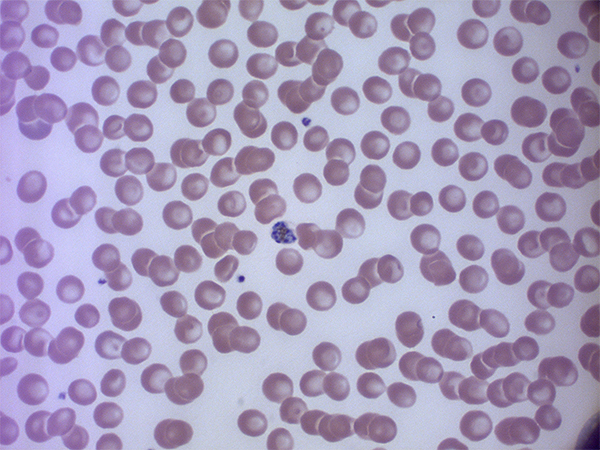
\includegraphics[width=0.48\textwidth]{images/malaria/f2_Pfalciparum}\vspace{1 mm}
	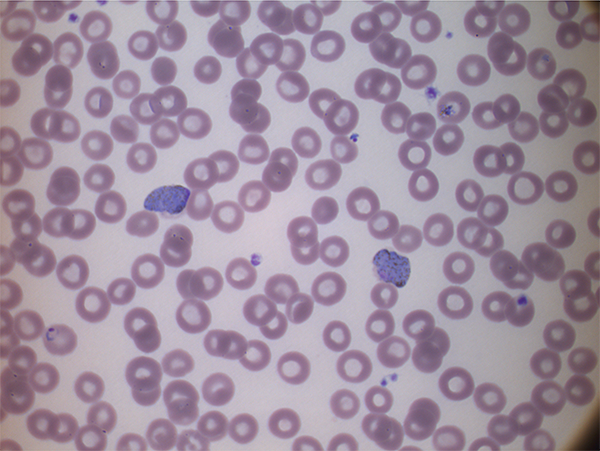
\includegraphics[width=0.48\textwidth]{images/malaria/f2_Pvivax}
	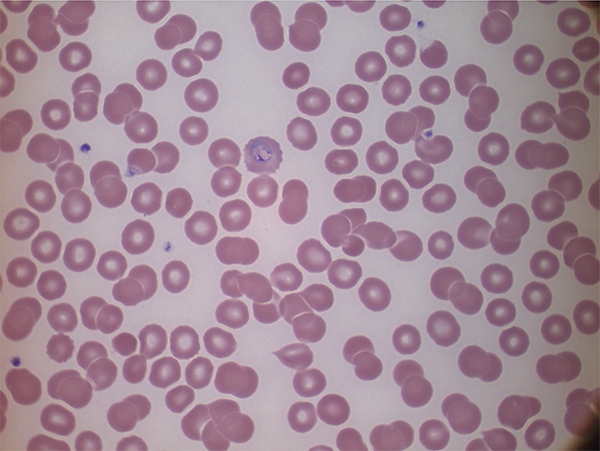
\includegraphics[width=0.48\textwidth]{images/malaria/f2_Povale}
	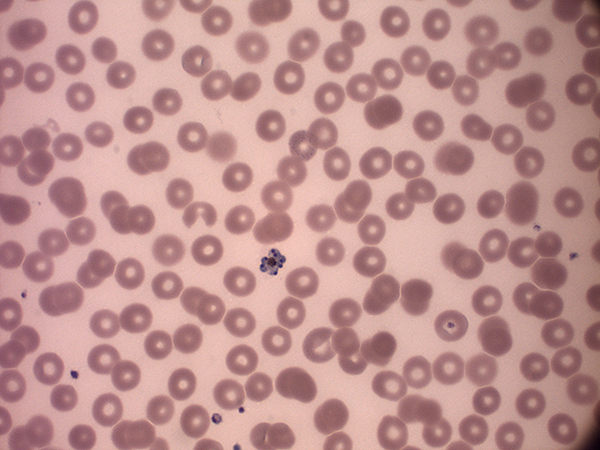
\includegraphics[width=0.48\textwidth]{images/malaria/f2_Pmalariae}
	\caption{\label{fig:malaria_types}Types of human malaria parasites: from left to right, \emph{P. falciparum} in its schizont stage, \emph{P. vivax} in two gametocytes specimens and one ring stage, \emph{P. ovale} in its ring stage, \emph{P. malariae} in its schizont stage.
		Courtesy of CHUV, Lausanne.}
\end{figure}

\section{Related Works}
% Pre Processing starts
In an image analysis field, especially when we refer to complex computer-aided pipelines, preprocessing methods are particularly used in order to improve the image data by suppressing unwanted noise or enhancing some image features for further processing.
It is worth mentioning preprocessing methods because they are an important step regarding the image analysis field, but, for what concerns the malaria-affected blood image analysis, in our review, we particularly found methods that operate for illumination correction and noise filtering purposes.
Generally speaking, digital~microscopy images can be acquired in different lighting conditions, with several types of acquisition devices or from blood smears stained with various staining protocols, and, consequently, the features of similar images could differ a lot.
Different techniques for illumination correction have been suggested to reduce such variation, e.g., a lot of authors work with grayscale-converted images as an illumination correction method.
On the other hand, noise filtering aims to remove the noise introduced by mishandling the slides and/or the camera settings.
Morphological operators have been extensively used as preprocessing for image enhancement in major studies.
Erosion and dilation operations on raw smear images allow for discarding undesired patterns and help in the selection of required cells or regions of interest. Morphological operators are useful for removal of unwanted
objects, holes filling, splitting, thinning and thickening. Different researchers during automated diagnosis of malaria used morphological operations in the preprocessing phase, and the most recent are listed below.

In \cite{Gonzalez2016}, Gonzalez-Betancourt et al. proposed a system to determine markers for watershed segmentation based on the Radon transform and mathematical operators. In the first step of the process, small irrelevant structures and part of the noise are eliminated by a morphological filter, in~order to ensure the preservation of the cells edges. Image smoothing is performed by a morphological erosion-reconstruction and dilation--reconstruction filter with a disk structuring element of a radius equal to 20 pixels, which is $0.274$ times smaller than the average radius of the RBCs. 

In this way, the influences of the size and the shape of the structures can be separated in the smoothing process. At the same time, the objects that are not eliminated remain unchanged. In addition, a morphological closing is performed with a disk structuring element having a radius smaller than half the average of the RBCs radii, in order to connect the possible (more than one) markers that can appear on a single cell.

In \cite{Kareem2012}, Kareem et al. illustrated a morphological approach for blood cell identification and use the image features such as intensity, histogram, relative size and geometry for further analysis. Before~the identification of blood cells, the authors  propose a novel morphological filtering based on the size of RBCs for platelets and/or artifacts elimination. A dilation is performed by a concentric ring structuring element and erosion by a disk-shaped structuring element. The radius of the structuring element depends on the radius of the RBCs, so that all the components smaller than the RBCs can be removed.

The system proposed in \cite{Oliveira2017} by Oliveira et al. is based on image processing, artificial intelligence techniques and an adapted face detection algorithm to identify Plasmodium parasites. The latter uses the integral image and haar-like features concepts, and weak classifiers with adaptive boosting learning. The search scope of the learning algorithm is reduced in the preprocessing step by removing the background around blood cells by means of morphological erosions both for training and for~testing.

Romero-Rondon et al. in \cite{Romero2016} presented an algorithm that uses morphological operations, the watershed method, the Hough transform and the clustering method of k-means to detect overlapped RBCs. In the preprocessing stage, white blood cells and platelets are removed before the segmentation task. During this step, some noise, the WBC cytoplasm and platelets still remain on the image. 
Therefore, the small objects are removed using a morphological opening and then the image is dilated with a disk-shaped structuring element.

Reni et al. in \cite{Reni2015} described a new algorithm for morphological filtering of the blood images as a preprocessing tool for segmentation. Conventional morphological closing on blood images removes the unwanted components but also useful information. On the contrary, the proposed method preserves the necessary information of foreground components while removing noise and artefacts.

In the method proposed in \cite{Sheik2013} by Sheikhhosseini et al., the first phase is the stained object extraction that detects candidates' objects that can be infected by malaria parasites using intensity and colour. Before detecting the stained objects, the method firstly extracts the foreground. The foreground image is a binary image that is produced after applying morphological hole filling on such pixels that have lower intensity value than average intensity value of the green layer. After the stained objects' extraction process, a series of morphological operations is also employed in order to eliminate small components and complete the final stained objects.

An edge-based segmentation of erythrocytes infected with malaria parasites using microscopic images is proposed by Somasekar et al. in \cite{Somasekar2015}.  A fuzzy C-means clustering is applied to extract infected erythrocytes, which is further processed for the final segmentation. A morphological erosion is used to erase some small noises and spots before the segmentation and holes inside the infected erythrocytes are filled using a morphological hole filling operation for the final segmentation.

In \cite{Tek2010}, Tek et al. presented a complete framework to detect and identify malaria parasites in images of Giemsa stained thin blood film specimens. In addition, the system is able to identify the infecting species and life-cycle stages.
The preprocessing step of the proposed method is applied to reduce the variations in the observed size, intensity, and colour of the cells and stained objects before the detection and classification steps. The aim is to correct the non-uniform illumination in the images. The estimation is based on a morphological closing operation using a sufficiently large structuring element. The sufficiently large size for an input image is determined automatically with respect to its average cell size computed from the area granulometry distribution.

Median filter is often used for reducing impulse noise. Several studies have used it to enhance microscopic images of peripheral blood smear towards characterization of malaria followed by adaptive or local histogram equalization. Local low pass filter and local adaptive histogram equalization techniques have also been applied to enhance the pathological image quality. Das et al. \cite{Das2015} showed that geometric mean filter provides better performance towards enhancing peripheral blood smear images. Di Ruberto et al. \cite{DiRuberto2016} proposed an approach to overcome the problem of uneven illumination conditions in image acquisition. For this purpose they designed an illumination pattern that simulates the classic visual defects introduced by the digital microscope lenses, that is the vignetting effect. Starting from the smallest radius, they applied different illumination patterns, created modifying the radius of the Gaussian curve, to the original images. Then, a similarity value measures the difference in terms of pixels between the original images and the corrupted ones.
% Pre Processing ends

% Segmentation starts
Segmentation is a key step in image analysis because it permits the identification and separation of the regions that compose an image, according to certain criteria of homogeneity and separation. Its~main target is to divide the image into parts that have a strong correlation with objects or areas of the real world contained in the image.
The commonly used segmentation methods essentially operate considering characteristics such as the brightness value, colour and reflection of the individual pixels, identifying groups of pixels that correspond to spatially connected regions. As for many problems of image processing, there is no standard solution valid in general, so different segmentation techniques can be applied, according to the characteristics of the images to process and of the objects to segment.
Medical images segmentation is typically performed using two main strategies: the first level aims to separate whole cells or tissues from the background and the second one aims to separate the tissue structure in different regions or the cell in their components, as the nucleus from the cytoplasm or intracellular parasites. The latter case is commonly used in applications in which the cell class depends on the morphological characteristics of its components.

%%% THRESHOLDING METHODS
Several other authors attempted to use thresholding combined with morphological operation as a segmentation method in their computer-aided systems, and they are described as follows.

Arco et al. in \cite{Arco2014} worked on thick blood films and proposed a method that uses an adaptive thresholding based scheme, which also allows an effective classification of pixels. This means that the election of whether a pixel belongs to the background or to the signal (parasites and white blood cells) is only established by the pixels around it, that is its neighbourhood. Then, morphological methods are applied to evaluate the area of connected components, labelling those belonging to parasites and counting their number.

Anggraini et al. \cite{Anggraini2011} proposed a method for separating blood cells, parasites and other components from the background in a microscopic field of a thin blood smear. They applied several global thresholding methods and visually compared the results to qualitatively determine which technique yields the best result. The binary image was then subjected to a hole filling morphological operator and applied as a marker to label blood cells. From each identified cell (RBC and WBC), constituents of the parasite (nucleus and cytoplasm) were extracted using multiple thresholds.

Dave et al. in \cite{Dave2017} performed image segmentation using histogram based adaptive thresholding followed by mathematical morphological operations (erosion and dilation). The detection of infected RBCs is based on an unsupervised learning technique.

The automated method proposed in \cite{Elter2011} by Elter et al. for parasite detection and identification worked on thin blood film acquired with Giemsa stain. The authors found that the G and B channels of the RGB colour are very good features to identify objects containing chromatin in Giemsa stained blood films, being not only considered highly discriminative but also almost independent of differences in illumination and staining intensity. They transformed the colour input image into a monochrome image \textit{I(x,y)}, which highlights objects containing chromatin: $ I(x,y) = arctan \frac{I_{green}(x,y)}{I_{blue}(x,y)} $. In this work, mathematical morphology has been used with a black top-hat operator to separate MP from both leukocytes and platelets, with a non-flat paraboloid structuring element with a radius of 9 and a slope of one~pixel. It should be taken into account that these fixed parameters might not be suitable for images with different pixel resolutions. The black top-hat operator is followed by a thresholding operation with a fixed threshold, which, according to the authors, is reliable given the independence of the G and B channels with regard to illumination and staining intensity. However, the authors do not define the value of this fixed threshold in their paper.

Kareem et al. in \cite{Kareem2011} used the Annular Ring Ratio transform method. Before applying it, a~preprocessing phase for removing platelets, parasites and other artefacts in the image has been performed. In the proposed method, the image after being converted to grayscale undergoes a morphological opening similar to closing. Unlike conventional closing (dilation followed by erosion), which uses the same structuring element, two different structuring elements are used: a concentric ring for dilation and a disk for erosion. The inner and outer diameter of the dilation ring is set to 35\% and 70\% of RBCs size, respectively, and the erosion disk has the same diameter. Therefore, considering that fixed manually defined parameters are used for this strategy, the results may substantially differ depending on the image resolution. This approach results in locating only the stained components in the image instead of all the cells and hence will not only speed up the operation but reduce the~complexity.

Mushabe et al.~\cite{Mushabe2013} used morphological and statistical classification to detect malaria in blood smears by identifying and counting red blood cells and Plasmodium parasites. Morphological~operations and histogram-based thresholding are used to extract RBCs
and boundary curvature calculations and Delaunay triangulation are used for splitting clumped RBCs. They worked on Giemsa-stained thin blood smears.

In \cite{Ross2006}, Ross et al. proposed a method that provides a positive or negative diagnosis of malaria and differentiates parasites by species. The segmentation step relies on a six step thresholding selection strategy. It aims to identify and segment potential parasites and erythrocytes from background. Mathematical morphology has been used in several key steps of the procedure. Hole~filling is used in the first step in order to fill RBCs' binary masks obtained from a first thresholding. \mbox{Afterwards, step 4} employs RBCs' morphological reconstruction with parasites' mask, found in step 2, for identifying infected cells. In step 5, a morphological opening filter, using a disk-shaped SE with a radius equal to the mean erythrocyte radius less the standard deviation, is applied to the grayscale, morphologically filtered, green component in order to remove any objects smaller than an erythrocyte. The morphological gradient (difference between a dilation and erosion of the image) is then calculated using a diamond-shaped SE with unity length.
Finally, in step 6, the intersection of morphological gradient image and the dilated cell cluster is calculated. This image is then transformed to a binary image by thresholding any value greater than zero. A series of morphological operations, namely a closing operation, thinning, and spur-removal are then applied to generate a contour of the segmented erythrocytes. Contours are filled, and the segmented mask is again reconstructed with the valid parasite marker image to result in a segmented mask of infected cells. RBCs and parasites masks are consequently ready for the next generation step.

Savkare et al. \cite{Savkare2011b} worked on thin blood films with Giemsa staining and used a global threshold and Otsu threshold \cite{Otsu} on grayscale enhanced image (green channel) for separating foreground from background. Hole filling has been performed on identified cells, and morphological operators have been used to identify overlapping cells. Then, a watershed transform has been applied for separating overlapped cells.

In addition, in the method proposed in \cite{Somasekar2017} by Somasekar et al., the segmentation of the infected parasites is based on thresholding. It is achieved in two stages by maximizing between-class variance of an original image and consequently by an iterative threshold selection from a stage-one threshold image with suitable stopping criteria. The segmented results are postprocessed to improve the accuracy of malaria parasites detection by morphological operators (erosion and closing).

% Morphology and/or granulometry in Segmentation stage:
On the other hand, a lot of works have been realized by means of mathematical morphology and/or granulometry in the segmentation stages, even in combination with thresholding strategies. They are briefly analysed below.

Ahirwar et al. \cite{Ahirwar2012} based their approach on thresholding and granulometry. The histogram of the complemented green component has been used, and it is said to be a bimodal distribution in all the considered images. Then, both local and global thresholds are used, and the union of the two binary images is chosen as the parasite marker image. A morphological opening filter, using a disk-shaped SE with radius equal to the mean erythrocyte radius less the standard deviation, is applied to the grayscale morphologically filtered green component of the image to remove any objects smaller than an erythrocyte. The morphological gradient is then calculated using a diamond-shaped SE with unity length. The segmentation method is applied to each object in the reconstructed binary image of erythrocytes individually. Those objects that do not exceed the area of a circle with a radius equal to the mean erythrocyte radius plus the standard deviation are regarded as being single cells, and are unmodified. On the other hand, the clumped cells are segmented as follows. First, the intersection of the morphological gradient image and the dilated cell cluster is taken. This image is then transformed to a binary image by thresholding any value greater than zero. A series of morphological operations, namely a closing operation, thinning, and spur removal are then applied to generate a contour of the segmented erythrocytes. The contours are filled, and the segmented mask is again reconstructed with the valid parasite marker image to result in a segmented mask of infected cells.

Di Ruberto et al. \cite{DiRuberto2002} aimed to detect the parasites by means of an automatic thresholding based on a morphological approach applied to cell image segmentation, which is more accurate than the classical watershed-based algorithm. They applied grey scale granulometries based on opening with disk-shaped elements, flat and hemispherical. They used a hemispherical disk-shaped structuring element to enhance the roundness and the compactness of the red cells improving the accuracy of the classical watershed algorithm, while they used a disk-shaped flat structuring element to separate overlapping cells. These methods make use of the red blood cell structure knowledge, which is not used in existing watershed-based algorithms.

Khan et al. in \cite{Khan2011} presented a novel threshold selection technique used to identify erythrocytes and possible parasites present on microscopic slides that greatly benefits from morphological operations, such as granulometry and morphological reconstruction.

In \cite{Rosado2017}, Rosado et al. proposed a system using supervised classification to assess the presence of malaria parasites and determine the species and life cycle stage in Giemsa-stained thin blood smears. For the RBCs segmentation, they used an adaptive thresholding approach followed by a closing morphological operation with an elliptical structuring element.

Soni et al. \cite{Soni2011} performed segmentation of erythrocytes by using granulometry as well. The~size and eccentricity of the erythrocytes are also required for the calculation of some feature values (as~these can be indicative of infection). The shape of the objects (circular erythrocytes) is known a priori, but the image must be analysed to determine the size distribution of objects in the image and to find the average eccentricity of erythrocytes present.
Grayscale granulometries based on opening with disk-shaped elements are then used. Non flat disk-shaped structural elements are applied to enhance the roundness and compactness of the red blood cells and flat disk-shaped structural elements applied to segment overlapping cells. The object to be segmented differs greatly in contrast to the background image. Changes in contrast can be detected by operators that calculate the gradient of an image. The gradient image can be computed and a threshold can be applied to create a binary mask containing the segmented cell. The binary gradient mask is dilated using a vertical structuring element followed by a horizontal structuring element. The cell of interest has been successfully segmented, but~it is not the only object that has been found. Any objects that are connected to the border of the image can be removed.

In Tek et al. \cite{Tek2010}, the localisation of the parasites is achieved after a foreground and background segmentation step. Firstly, a rough foreground image using morphological area top-hats (using the average cell area value) is extracted. Then, from these rough foreground and background regions, two different threshold values are determined and used in morphological double thresholding of the input grey level image to produce a refined binary foreground mask. From the foreground image, the stained pixels are detected using again a thresholding approach and finally used as markers to extract the stained objects by morphological area top-hats based on the estimated average area value.

In \cite{Yunda2012}, Yunda et al. proposed a method for \textit{P. vivax} parasite detection. The segmentation phase is a combination of border and region detection that allows rejection of the image background and permits identifying each of the objects. Initially, the morphological gradient method is used to enhance the borders of previously found objects. This is followed by a threshold detection stage using the K-Median method.
Furthermore, a Laplacian operator was used to discriminate the pixels that are interior or exterior in relation to the regions of the images and then erosion operation followed by two dilations were applied to delete the pixels that did not make up part of any object. In the end, Absence~of Gradients and Nernstian Equilibrium Stripping (AGNES) and K-Median techniques were applied to assign the remaining number of pixels to each region, using the image regions previously identified as objects and background as the starting point.

Several authors used marker controlled watershed \cite{Soille2004} with morphological approach, as~described in the following.

Das et al. in \cite{Das2011,Das2013,Das2014,Das2015} segmented erythrocytes as aforesaid and then morphological operators are used to eliminate unwanted cells like leukocytes and platelets. Moreover, overlapping erythrocytes are segmented by using a marker controlled watershed segmentation technique.

In \cite{Devi2017}, Devi et al. proposed a computer assisted system for quantification of erythrocytes in microscopic images of thin blood smears. The performance of the system in classifying the isolated and clump erythrocytes by geometric features is evaluated for the different classifiers. The clump erythrocytes are segmented using marker controlled watershed with h-minima as internal marker.

In \cite{Dey2015}, Dey et al. presented an automatic system for segmenting platelets, useful for identifying disease as malaria, using a colour based segmentation and mathematical morphology (opening~operations with a disk element of radius 2).

In the study presented in \cite{Diaz2009} by Diaz et al. for quantification and classification of erythrocytes in stained thin blood films infected with \textit{Plasmodium Falciparum}, the authors used connected morphological operators in the segmentation step. The RBCs are detected as follows: firstly, a pixel classification allowed for labeling each image pixel as either background or foreground, based on its colour features. Afterwards, an inclusion-tree structure is used to represent the hierarchical object relations between background and foreground so that a filtering process allows for removing irrelevant structures such as artefacts generated at the staining or digitization processes.

Khan et al. \cite{Khan2011}, among other experimentations, used it in order to try to separate overlapping cells because, according to their statements, watershed transform can separate touching cells, but it is not sufficient for overlapping cells.

In the algorithm described by Romero-Rondon et al. in \cite{Romero2016}, the detection of overlapped RBCs is still based on marker-controlled watershed transform. To define the suitable markers in watershed transform, they used three different approaches, based on a morphological erosion operation, on Hough transform and on a clustering method of K-means.

{Savkare et al. in \cite{Savkare2015} segmented cells using K-mean clustering and global threshold. Overlapping~cells} are separated using a Sobel edge detector and watershed transform. Watershed transform is applied on each cluster separately. Over-segmentation is minimized by a series of morphological operations, like~erosion and dilation utilizing disk-shaped structuring elements.

In \cite{Savkare2011a}, an approach  to detect red blood cells with consecutive classification into parasite infected and normal cells for further estimation of parasitemia is proposed. For separation of overlapping cells, watershed transform is applied on a distance transform of binary mask of cells having a larger area.

In \cite{Springl2009}, {\v{S}}pringl performed red blood cell segmentation by using marker-controlled watershed transformation based on the image gradient. Markers are computed as a combination of the binary mask of the red blood cells and centres of the cells that are computed using a similar algorithm that was utilized for the evaluation of the average cell radius. The binary mask is obtained by thresholding the grayscale image with an automatically estimated threshold using the Otsu method \cite{Otsu}.

In \cite{Sulist2015}, Sulistyawati et al. combined morphological operations (erosion, dilation, opening and closing) and blob analysis to segment and identify malaria parasites with a high degree of accuracy.

Tek et al. in \cite{Tek2006} proposed a classifier-based method for the segmentation stage, which relies on a Bayesian pixel classifier to distinguish between stained and non-stained pixels. In particular, they used a non-parametric method based on histograms in order to produce the probability density functions of stained and non-stained classes. Stained pixels can belong to other components such as WBCs, platelets or artefacts, in addition to the parasites, and so the detection procedure requires a further classification to distinguish among parasite and non-parasite pixels. However, the stained pixels have to be represented as connected sets, representing stained objects, to extract features for the classifier. Furthermore, top-hat extraction and infinite reconstruction were applied to find the regions that include the objects.

To sum up, the analysed systems use mathematical morphology methods during or immediately following the segmentation step for the following purposes:
% TODO inserire tabella

% Segmentation ends 

% Feature extraction starts
Feature extraction has the aim of reducing the computational complexity of the subsequent process and facilitating a reliable and accurate recognition for unknown novel data, considering~that the input data to an algorithm could be too large to be processed and it could be redundant (e.g., repetitiveness of pixels patterns in an image). Moreover, the in-depth understanding of the domain-specific knowledge gained by human experts on the problem being addressed can be of extreme importance for the design of a reliable and effective feature extraction engine \cite{Jiang2009}.
It starts from determining a subset of the initial features, and this procedure is called feature selection. The~selected features are expected to contain the relevant information from the input data, so that the desired task can be performed by using this reduced representation instead of the complete initial data.
Malaria~parasite infection causes micro structural changes in erythrocytes. The microscopic features of the RBCs are usually specific to morphology, intensity and texture. They may also represent the differences that occur among healthy and unhealthy cells. Most of the studies have reported both textural and geometric features for describing malaria infection stages \cite{Das2015}.
Generally speaking, features may be distinguished according to the following characteristics: morphological features and textural and intensity features.

It is a well known mathematical morphology approach to compute a size distribution of grains in binary images, using a series of morphological opening operations. It is the basis for the characterization of the concept of size. Some authors used area granulometry for preprocessing purposes in malaria characterization \cite{Tek2010}, even though it is certainly effective for extracting cell size features' information \cite{Springl2009,Tek2006,Malihi2013}. In \cite{Tek2010}, local area granulometry combined with colour histogram are used as features. The area granulometry feature is calculated locally on the binary mask of the stained objects, for the RGB channels, and then concatenated. Morphological features are also used in \cite{Ross2006} (erosion dilation), in \cite{Das2011} (opening, closing) and in \cite{DiRuberto2002} (skeleton) to classify parasites.
% Feature extraction ends

\begin{figure}[!t]
	\centering
	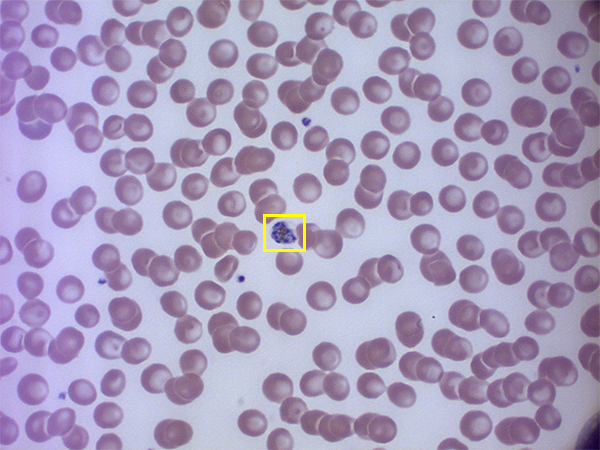
\includegraphics[width=6.5cm]{images/malaria/f2_Pfalciparum_rect}
	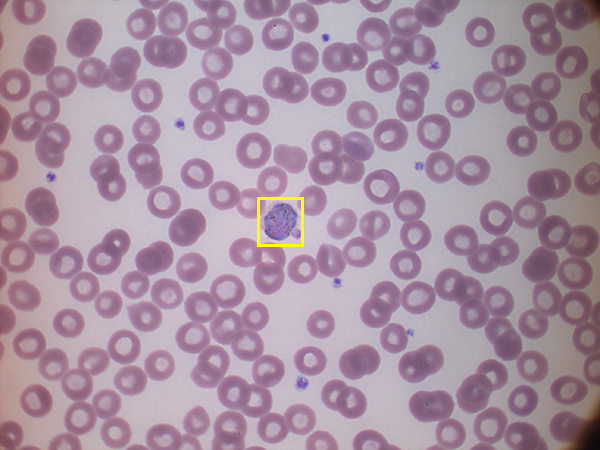
\includegraphics[width=6.5cm]{images/malaria/f2_Pvivax_rect}
	\includegraphics[width=6.5cm]{images/malaria/f2_Povale_rect}
	\includegraphics[width=6.5cm]{images/malaria/f2_Pmalariae_rect}
    \includegraphics[width=2cm, height=2cm]{images/malaria/f2_Pfalciparum_crop}
	\includegraphics[width=2cm, height=2cm]{images/malaria/f2_Pvivax_crop}
	\includegraphics[width=2cm, height=2cm]{images/malaria/f2_Povale_crop}
	\includegraphics[width=2cm, height=2cm]{images/malaria/f2_Pmalariae_crop}
	\caption{\label{fig5_malaria_types}Types of malaria parasites: from top left, clockwise, \emph{P. Falciparum} in its schizont stage, \emph{P. Vivax} in a gametocytes specimen, \emph{P. Malariae} in its schizont stage, \emph{P. Ovale} in its ring stage. All parasites have been surrounded with a yellow box. Underneath, from left to right: crops of P. Falciparum schizont, P. Vivax gametocyte, P. Ovale ring and P. Malariae schizont, taken from the boxes. Courtesy of CHUV, Lausanne.}
\end{figure}

\begin{figure}[!b]
	\centering
	\includegraphics[width=2cm, height=2cm]{images/malaria/falciparum_1_ring}
	\includegraphics[width=2cm, height=2cm]{images/malaria/falciparum_2_trophozoiteAge}
	\includegraphics[width=2cm, height=2cm]{images/malaria/falciparum_3_schizont}
	\includegraphics[width=2cm, height=2cm]{images/malaria/falciparum_4_gametocyte}
	
	\includegraphics[width=2cm, height=2cm]{images/malaria/ovale_1_ring}
	\includegraphics[width=2cm, height=2cm]{images/malaria/ovale_2_trophozoite}
	\includegraphics[width=2cm, height=2cm]{images/malaria/ovale_3_schizont}
	\includegraphics[width=2cm, height=2cm]{images/malaria/ovale_4_gametocyte}
	
	\includegraphics[width=2cm, height=2cm]{images/malaria/vivax_1_ring}
	\includegraphics[width=2cm, height=2cm]{images/malaria/vivax_2c_trophozoiteDeveloped}
	\includegraphics[width=2cm, height=2cm]{images/malaria/vivax_4_gametocyte}
	\caption{\label{fig6_malaria_stages}Examples of malaria parasite stages. From top left: P.falciparum ring, trophozoite, schizont, gametocyte;
		P.ovale ring, trophozoite, schizont, gametocyte; P.vivax ring, developed trophozoite, gametocyte. \cite{Loddo2018}}
\end{figure}

\section{Parasites morphology}
A blood smear image, obtained through a microscope, is presented in fig. \ref{fig4_colour}. It typically contains at least three regions of interest: white blood cells (or leukocytes), red blood cells (or erythrocytes) and platelets (or thrombocytes). Two different categories of leukocytes exist: granulocytes (composed, in turn, of neutrophils, basophils and eosinophils). On the other hand, leukocytes without granules are called agranulocytes (composed of lymphocytes and monocytes). Erythrocytes do not have any subcategory even though malaria parasites (MPs) can infect them, consequently modifying their shape, morphology or colouration conditions. In particular, fig. \ref{fig5_malaria_types} shows several examples of malaria parasites in their different life stages and type.
Although MPs infect only RBCs, a blood smear image representing both WBCs (particularly granulocytes) and MPs could be very difficult to analyse because of the similarities in colouration and shape between parasites and WBC grains, as shown in fig. \ref{fig4_colour}.

\begin{figure}[!t]
	\centering	
	\includegraphics[width=8cm]{images/malaria/f2_typical_bb}
	\caption{\label{fig4_colour} Example of blood smear image acquired with a good colouration and illumination scheme. The image is characterized by three different regions of interest: a eosinophil granulocyte on bottom left (yellow bounding box), a schizont Plasmodium Falciparum on bottom centre (green bounding box) and the erythrocytes. Please note that some platelets are also present (blue bounding box). Courtesy of CHUV, Lausanne.}
\end{figure}
MP-IDB collects four malaria parasite species: Plasmodium Falciparum, Ovale, Malariae and Vivax, in four different life-cycle stages: ring, trophozoite, schizont and gametocyte. It must be noted that Plasmodium Falciparum trophozoite and schizont are very rare and they are not present in our data collection. A complete set of examples, extracted from the dataset, are shown in fig. \ref{fig6_malaria_stages}. The life-cycle-stage of the parasite is defined by its morphology, size and the presence or absence of malarial pigment. The species differ in the changes of infected cell’s shape, presence of some characteristic dots and the morphology of the parasite in some of the life-cycle-stages \cite{Somasekar2011}.
An automated malaria parasites analysis on blood smears usually comprises four different tasks, as follows:
\begin{enumerate}  
	\item Image preprocessing: the images are normalized in colouration, because it can differ a lot from image to image, and the different regions of interest are made the most contrasted possible. 
	\item Segmentation: red blood cells and/or parasites are separated from the background and white blood cells by using algorithms based on different characteristics of the cells (e.g. shape, colour, texture).
	\item Feature extraction: relevant characteristic (e.g. shape, colour, texture) are extracted from the different region of interest in order to train an automatic parasite analyser.
	\item Classification: several classification schemes can be performed. Hierarchically, cells are classified in red blood cells and white blood cells. Afterwards, red blood cells are classified in affected from parasite(s) or not. In the end, parasites are classified in their type and life stage. Parasites potentially can also be present outside the cells. In this case, they should need a more specific and dedicated analysis.
\end{enumerate}

\begin{figure}[!t]
	\centering	
	\includegraphics[width=2.9cm]{images/malaria/f1a}
	\includegraphics[width=2.9cm]{images/malaria/f1b}
	\includegraphics[width=2.9cm]{images/malaria/f1c}
	\includegraphics[width=2.9cm]{images/malaria/f1d}
	\caption{\label{f1_img_types} Different illumination conditions could generate unconventional colour schemes in images. This is due to the absence of a standardized acquisition procedure. From left to right: same smear acquired with four microscope brightness levels. Courtesy of CHUV, Lausanne.}
\end{figure}

\chapter{WBCs Segmentation}
The main purpose of this thesis was to develop a CAD system able to extract appropriate and useful information from blood cell images, acquired by means of microscopes, in order to easily perform activities on them, e.g., the WBCC. In particular, we aimed to realize a dataset-independent framework for cells analysis, a precise scheme of cells labelling and counting and a complete cells classification for diagnostic tasks.
The proposed method starts with a segmentation step, which is a crucial step in this procedure because its accuracy greatly affects both the computational performances and the whole system's overall accuracy. However, it is also a very difficult problem to manage because of the complex nature of the cells, low resolution of microscopic images and complex scenes, e.g. cells can overlap each other or cells can have different sizes or shapes. On the other hand, the colour and contrast between the cells and the background can vary so often according to the frequent, inconsistent staining technique, thickness of smear and illumination. Although standardization is useful to avoid superfluous differences in the features of similar images, a robust segmentation approach can cope with the described issues and this is certainly one of the main motivations to the realization of this work.
Referring to the state of the art, it is clear that most of the authors proposed classic methods in order to perform cells segmentation, like thresholding. In some cases, WBCs counting has been based on detection methods rather than on segmentation ones, by using the circular Hough transform \cite{Mahmood} or texture analysis, even though colour image segmentation could even be performed with pixels clustering or classification in colour space. Unsupervised and supervised schemes \cite{Pan}, such as k-means and neural networks, have been widely used for this purpose even if there are many disadvantages to deal with. Generally, the biggest problem of an unsupervised clustering scheme is how to determine the number of clusters, which is known as cluster validity. And as for a colour image, the selection of colour space is quite critical. The supervised scheme needs training. The training set and initialization may affect the results, and overfitting should be avoided. So a supervised clustering/classification algorithm with good generalization property is most appealing. Our method aims to solve the segmentation problem in a non-linear feature space obtained by kernel methods in order to overcome the non-linearity of data distribution and the shift/offset of colour representing the different regions of interest inside a blood sample: mature erythrocytes, leukocytes nuclei and cytoplasm. SVM (Support Vector Machines) and ANN (Artificial Neural Network) are machine learning models with excellent performances in classification, but their main drawbacks are that a training phase is absolutely necessary to make them work and it could be computationally hard with large datasets.
Moreover, two main levels can be distinguished for peripheral blood images segmentation: the "cells level", which aims to separate whole cells from the background (or plasma) and the "intra-cells level" that tries to separate the various cells components, such as the nucleus from the cytoplasm or intracellular parasites. Several authors have proposed methods for effective segmentation of the nucleus of leukocytes, while there are few attempts of segmentation of the cytoplasm. In this chapter the segmentation techniques used to segment the whole white blood cells will be illustrated. Since during the analysis of the images and the segmentation results many issues have been observed, different approaches have been proposed in order to make further improvement and to obtain better result. Most of the proposed approaches are based on machine learning methods. Although in many cases machine learning methods are not considered computationally suitable for segmentation, here special effort has been devoted to improve this kind of approaches in order to be robust against uneven illumination, local imprecision, different acquisition devices and staining. They have been chosen mostly because they can provide excellent segmentation results by letting them train with different samples. Efforts have also been made to reduce their computational expensiveness.
  
\section{SVM pixel classification for segmentation} \label{iciap2015} %ICIAP 2015
The first realised method for white blood cells segmentation makes us of a combination of Support Vector Machine pixel classification strategy for segmentation purposes, associated with a ROI selection to give SVM sufficient and precise manual samples for its training phase. 
The first step of the algorithm is to apply a classic segmentation method (Otsu thresholding) in order to obtain pure samples related to the four most important regions: one representing the leukocytes nucleus and cytoplasm, the mature erythrocytes and the background. As a comparison, we have also realized a method based on three Mean Shift iterated procedures in order to search the clustering modes corresponding to the aforementioned four regions colours. Afterwards, we prepared the training samples by sampling the regions obtained from the thresholding phase so as to perform the training process of a multi-class SVM in order to correctly classify all the pixels of a given image. Finally, the SVM is used to segment the image for extracting whole white blood cells, using a classification phase by means of a model. Since the size of training set could be controlled and reduced in advance during the sampling procedure, SVM training is really fast.

\subsection{On Mean Shift Technique}
Mean Shift technique was originally proposed in 1975 by Fukunaga \cite{fukunaga}, then adapted by Chen \cite{Pan} and generalized for image analysis purposes. More recently it have been extended to low-level vision problems \cite{Foran}, including segmentation, adaptive smoothing and visual tracking. Basically, it is used as a non-parametric technique for the estimation of the density gradient in image analysis field, even if it was developed in order to perform mode finding on clustering procedures. In contrast to the classic K-means clustering approach, there are neither a priori assumptions about the point distribution nor the number of modes and clusters: they are computed by the Mean Shift procedure itself. Furthermore, Mean Shift has been adapted to become a very effective image segmentation technique, even if it was born as a clustering method of data analysis. It allows to attenuate shape or colour differences between the objects inside the considered images; for these reasons it works as a local homogenization technique. Considering its operating principles, the objective is to substitute every single pixel value with the mean of the sampled pixel values in a certain neighbourhood, within a certain radius $R$ and a certain colour distance $D$; both of them are usually input defined by the user which generally has a deep knowledge about the context or uses some pre-processing technique to obtain the best values of $R$ and $D$. Typically, Mean Shift requires at least three basically information to gain the best results; first of all, we have to define a certain kernel, which uses a distance function, to measure the pixel distance in every single iteration of the procedure: examples are the Gaussian kernel and the Epanechnikov kernel. Secondly, it needs two distance values: an $R$ radius and a $D$ colour distance. Then, iteratively, the procedure finds the modes of an input given image and calculates new values for every single pixel, according to the chosen kernel function and the distance parameters. It is worth mentioning that Mean Shift algorithm is not well defined at the boundaries, because it does not consider the non-existent neighbour pixels. Consequently, a strategy to handle them is necessary. For example, we have studied a padding of the image to process boundary pixels correctly.

\subsection{Experimental evaluation}
Remembering that our starting objective was to segment white blood cells, now we explain how this classification method can be used to reach our segmentation purposes and targets. Support Vector Machine (SVM) has been chosen in order to perform a classification of every single pixel belonging to the images we have to segment, according to the method proposed in \cite{Pan}. Once the Mean Shift has been performed on a certain training set, we use a set of these produced images to train the different SVM we realized. As a comparison, we also segment every single dataset image with classic segmentation methods. It is done to execute a more in-depth analysis of our study. The \textbf{first strategy} works as a normal binary SVM classifier, hence we have exactly two classes in which the pixels will be classified: the positive class groups together the white blood cell nuclei and cytoplasm pixels, instead the negative class represents pixels belonging to erythrocytes or background. Fig.~\ref{fig:exs1} shows the segmentation result using this solution, in which the WBC is exactly recognized and segmented, but the lighter region of erythrocytes is misclassified as WBC region. The \textbf{second strategy} substantially works like the first one, with the main difference that we exclude from the training samples all the pixels belonging to the cytoplasm, in order to avoid misclassification due to similarities with the lighter region of erythrocytes. Fig.~\ref{fig:exs1} shows the segmentation result using this solution. Again the nucleus is well detected but for determined classes of WBCs the cytoplasm is not well detected. The \textbf{third strategy} is based on the results obtained with the two previous versions. In fact the classifier needs more valid training samples for cytoplasm only. So, in last version we perform a three-class SVM, using both the pixels belonging from WBCs nuclei (class 1) and both pixels belonging to the WBCs cytoplasm (class 2). Thus, pixels belonging to erythrocytes or background are labelled with class 3. Note that for this approach only classic segmentation have been used to produce pure samples for the SVM, because Mean Shift segmentation merge together both WBC nucleus and cytoplasm. A Mean Shift alteration could be done to adapt it for our purposes, but we have chosen to use classic method for simplicity. Fig.~\ref{fig:exs1} and shows the segmentation result using this solution in which both nucleus and cytoplasm are well detected.

\begin{figure}[h]
	\centering
	\hspace{-1.5mm}\includegraphics[width=0.14\textwidth]{images/2015_1_caip/3-1}\vspace{1 mm}
	\includegraphics[width=0.14\textwidth]{images/2015_1_caip/3-2}
	\includegraphics[width=0.14\textwidth]{images/2015_1_caip/3-3}
	\includegraphics[width=0.14\textwidth]{images/2015_1_caip/1-1}
	\includegraphics[width=0.14\textwidth]{images/2015_1_caip/1-2}
	\includegraphics[width=0.14\textwidth]{images/2015_1_caip/1-3}
	\includegraphics[width=0.14\textwidth]{images/2015_1_caip/2-1}
	\includegraphics[width=0.14\textwidth]{images/2015_1_caip/2-3}
	\includegraphics[width=0.14\textwidth]{images/2015_1_caip/2-4}
	\includegraphics[width=0.14\textwidth]{images/2015_1_caip/4-1}
	\includegraphics[width=0.14\textwidth]{images/2015_1_caip/4-2}
	\includegraphics[width=0.14\textwidth]{images/2015_1_caip/4-3}
	\caption{\label{fig:exs1} (Top) From left to right: training original image from ALL-IDB2, manually segmented nucleus and cytoplasm; test original image, segmentation result for nucleus an cytoplasm with the first strategy. (Bottom) From left to right: test original image, segmentation result for nucleus an cytoplasm with the second strategy; test original image, segmentation result for nucleus an cytoplasm with the third strategy}
\end{figure}

\subsection{System Implementation}
For each strategy, the training set is formed by sampling pixels from the images belonging to the ALL-IDB2 presenting healthy WBCs chosen to make part of the available training images. On the other hand, the test set is formed of the first 33 images of ALL-IDB1, acquired in the same lighting conditions and with the same camera. 

%\subsection{First Step}
According to the prior knowledge defined about Mean Shift and classic segmentation methods, we have used two strategies to perform the first phase of our algorithm. Both of them are focused to offer the SVM a sufficient set of possible training samples. We have used either classic methods or Mean Shift to obtain this training set. The main objective is to understand which samples represent the most accurate pixels to train an SVM model between Mean Shift and thresholded images. As said before, we have used both the approaches to experiment their behaviour in relation to the SVM training set building. With thresholding, we have obtained two binary masks. The first one contains the white blood cells segmented in their entirety while the second one contains only the white blood cells nuclei.
From these images, the segmented cytoplasm region could be easily obtained performing a difference operation between the first image and the second one and remembering that the cytoplasm region is always placed around the white blood cell nucleus. Thanks to this process we can easily perform the SVM training phase. Overall, we have obtained, in both cases, a certain set of images in which the regions have been pointed out. Mean Shift method, instead, produces only a set of images in which the regions of interest are marked with different colours, obtained by finding the dominant colour modes of the three main regions: erythrocytes, white blood cell and background. 

\begin{figure}[!b]
	\centering
	\includegraphics[height=0.10\textheight]{images/2015_2_iciap/Im002_1}
	\includegraphics[height=0.10\textheight]{images/2015_2_iciap/Im002_1_MS}
	\includegraphics[height=0.10\textheight]{images/2015_2_iciap/Im002_1_T}
	\caption{\label{fig:svm_candidates} Examples of training samples candidates. From From left to right: original image from ALL-IDB2, same image after three iteration of Mean Shift algorithm; same image thresholded to empathize WBC nuclei (light blue) and cytoplasm (blue).}
\end{figure}

%\subsection{Second Step}
At this time, our interest is to perform a properly training phase over the given pixels obtained in phase one. The chosen pixels must be the most various possible all over the regions obtained in phase one, in order to realize a proper classification model during SVM training phase. 
The strategy we followed to train the SVM in order to produce a classification model is now presented. Once we have obtained pixels belonging to cytoplasm, white blood cell nucleus and red blood cells regions, the remaining step to perform is to accurately choose these pixels with a uniform sampling, in order to consider every single image available in the group of images given for the training set.
Thus, four different regions form candidates of training set for SVM. We mark nucleus pixels of white blood cells with class label $I_1$, cytoplasm pixels with class label $I_2$, instead mature erythrocyte and non-cell region pixels are marked with $I_3$. To avoid uncertainty, the following property has been set:$ I_1\cap I_2 \cap I_3 = \emptyset$ (empty set). SVM implements a classification strategy that exploits a margin-based “geometrical” criterion rather than a purely “statistical” criterion. It does not estimate the statistical distributions of classes for classification, while defines the classification model by exploiting the concept of margin maximization. There are two types of margin in SVM. Hard margin classifier works well in no-noise cases, but fails with noisy data due to overfitting. Soft margin classifier may achieve much better generalization results by relaxing the hard margin and ignoring the noisy data. So, removing noisy samples from the training set may benefit to training; for this reason we have produced pure samples of the three classes. Statistics theory has revealed that, through uniform, or Monte Carlo sampling, a subset could be produced to represent the entire data set approximately while retaining the distribution of data effectively \cite{caflisch}.
The essential steps of this phase can be summarized as follows:
\begin{itemize}\itemsep3pt \parskip0pt \parsep0pt
	\item[-] sample N pixels from $ I_1, I_2, I_3$ regions. There are N/4 pixels sampled respectively from four regions (cytoplasm, nucleus, mature erythrocytes and background region) to keep the size of the training set balanced;
	\item[-] train a SVM online, taking the reduced training set defined at point one and a RBF kernel and generate a classifier model;
	\item[-] use this model to classify the image pixels which are represented by $(R,G,B)^T.$
\end{itemize}	
We have performed two main experiments. The first one has been realised to verify our implementation performances over single WBCs and in order to identify the most suitable parameters for the SVM. Thus, through a 10 fold cross-validation each time we have divided the original training set in two subsets, the first one to train the SVM and the second one to test the obtained model. An ideal average accuracy value has been reached by choosing the parameters $c$ and $\gamma$ as $1e3$ and $1e1$ respectively. 
The second and final experiment have been realised to verify the segmentation performances of the proposed method. Thus the whole original training set has been used to create the SVM model. The first 33 native resolution images has been used as test set and to check the method applied to a natural image composed of several white blood cells of many different classes. 

%\subsection{Third Step}
Once the first (visual) results have been obtained we have started experimenting with various features that can be used to train the classifier.
In fact, even though we are talking of a segmentation technique, pixels are used as features for the SVM classifier. Until now the only descriptors used are the original RGB colour intensity values. Although, in many cases, these features are enough to reach a good segmentation result, in other cases a poor feature set like this is not able to discriminate pixels belonging to regions with wide variations in colours. Thus the first intuition has been to add the average colour values of each pixel neighbourhood. These average values have been tested for neighbourhood of size $3 \times 3$, $5 \times 5$ and $7 \times 7$. For the same neighbourhood we have also computed other statistical features that are often used for segmentation purposes: standard deviation, uniformity and entropy. While the segmentation accuracy highly benefits from the use of these new features, the overall system became slower, both in training and in segmentation phases. Furthermore, the step of samples selection, used to train the classifier, became too complex, due to a higher number of samples with different values. For all these reasons the features previously mentioned have been extracted only for neighbourhood of size $3 \times 3$, showing excellent performances as showed in fig.~\ref{fig:ex5}, outperforming previous results. After the segmentation, all the images have been automatically cleaned, as we have already proposed in \cite{Put13c}, in order to remove small artefacts from the background and to give to the reader an idea about the goodness of the results.
In order to evaluate the segmentation performances of the proposed method, a subset of images (10 random samples) belonging to the ALL-IDB1 have been manually segmented by skilled operators, creating two ground-truth images for each sample. These images display respectively each blood cell present in the image and the white blood cell nuclei. Fig.~\ref{fig:ex5} shows some images belonging to the ALL-IDB1 and their relative ground-truth images.
\begin{figure}[!b]
	\centering
	\includegraphics[height=0.18\textwidth]{images/2015_1_caip/Im003_1}
	\includegraphics[height=0.18\textwidth]{images/2015_1_caip/Im003_1_WBC}
	\includegraphics[height=0.18\textwidth]{images/2015_1_caip/Im003_1_WBCn}
	\includegraphics[height=0.18\textwidth]{images/2015_1_caip/Im003_1_label}
	\caption{\label{fig:ex5}Original images from the ALL-IDB1 database, ground-truth for whole leukocyte, ground-truth for leukocyte nuclei and final segmentation result.}
\end{figure}
Finally, the ground-truth images previously described have been compared with the automated segmented images in order to calculate the most common metrics for segmentation evaluation, that are: accuracy, sensitivity, specificity, precision and F-measure. Our segmentation approach has been compared with some well know segmentation algorithms like Otsu \cite{Otsu} and Zack \cite{Zack}. Table~\ref{tab:table1} shows the average performances obtained with the ten tested samples. As it can be seen the most important values obtained with our approach are higher than the other segmentation approaches. 
\begin{table*}[!b]
	\caption{Segmentation performances.}
	\centering\tabcolsep=2mm
	\begin{tabular}{ccccccccc}
		\hline
		&	Otsu 			 &			Zack 				&	Our Approach\\
		\hline
		Accuracy	&   77.67 $\pm$  0.6	 &		74.76	$\pm$  3.6 		&	    97.61 $\pm$  1.7\\
		Sensitivity 	&   76.70 $\pm$  8.3 	 &		85.43	$\pm$  6.8	 	&	    98.45 $\pm$  0.3\\
		Specificity	&   85.62 $\pm$  4.6	 &	 	81.27	$\pm$  5.4	 	&	    97.56 $\pm$  1.2\\
		Precision  	&   53.55 $\pm$  12.8 &		79.12	$\pm$  8.6	 	&	    70.45 $\pm$  5.8 \\
		F-measure 	&   45.18 $\pm$  5.3	 &	 	55.15	$\pm$  3.3	 	&	    82.13 $\pm$  2.3\\
		\hline
	\end{tabular}
	\label{tab:table1}
\end{table*}

\section{Multi-class SVM segmentation} \label{caip2015}  % CAIP 2015
This segmentation solution has been developed by following the idea described in the previous chapter and improving it.
Basically, the same settings of the previous schema have been maintained, from the dataset to materials. Method is following presented.
The first step of the algorithm is to apply a classic segmentation method to obtain pure samples related to the regions of white blood cells nucleus and cytoplasm, mature erythrocytes and background. The pixels obtained from these regions have been reduced in number through a Nearest Neighbour  Search (NNS) by removing any duplicates or elements with distance next to zero. Even in this case, SVM has been chosen due to the excellent results of the previous method. Once the manually segmented images have been obtained on a certain training set, we used a set of these produced images to train the different SVM we realized. Then, we tuned three different strategies. 
The \textbf{second strategy} basically works like the first one, with a main difference. We have excluded, indeed, from the training samples all the pixels belonging to the cytoplasm, in order to avoid misclassification due to similarities with the lighter region of erythrocytes. 
The \textbf{third strategy} is based on the results obtained with the two previous version. In fact the classifier needs more valid training samples for cytoplasm only. So, in this version we performed a three-class SVM, using both the pixels belonging from WBCs nuclei (class 1) and both pixels belonging to the WBCs cytoplasm (class 2). Thus, pixels belonging to erythrocytes or background are labelled with class 3. 
It is well know that getting manually segmented images is neither simple nor cheap. Considering that, we perform an experiment which can be be applied to every peripheral blood images dataset, even in each illumination condition and with different combinations  of cameras and microscopes. 
Our propose is based on ROI (Region of Interest) selection. Thus, making use of few original images the object of interest (WBCs) could be selected and used as positive example for our multiple classifier. Considering that we are talking of a segmentation method based on classifiers also negative instances are needed, so the background region, that comprises red blood cells and plasma, must be selected. An example of ROI selection for positive and negative example is showed in Fig.~\ref{fig:ex6}.

\begin{figure}[!b]
	\centering
	\includegraphics[height=0.25\textwidth]{images/2015_1_caip/ROI1}
	\includegraphics[height=0.25\textwidth]{images/2015_1_caip/ROI2}
	\includegraphics[height=0.25\textwidth]{images/2015_1_caip/ROI3}
	\caption{\label{fig:ex6}Examples of ROI selection for WBCs, RBCs and plasma.}
\end{figure}

Obviously, the negative samples must not contain any WBC. In fact, in this case the NNS is performed also over pixels belonging from different region, in order to avoid errors committed during the ROI selection and in order to remove pixels with close values. In this way, the obtained training set certainly present uniformly distributed pixel values. Note that with this approach the WBC cytoplasm and nucleus are managed as a unique region, both because the ROI selection is not so suitable for adjacent regions and both because they can be easily separated in a further step by using a simple threshold. Differently from other approaches, we are now able to take also RBCs into account, considering them as a different class.
Thus it is possible to perform a binary segmentation or a multiple segmentation as showed in Fig.~\ref{fig:ex7}.

\begin{figure}[!t]
	\centering
	\includegraphics[width=0.49\textwidth]{images/2015_1_caip/ROI4}
	\includegraphics[width=0.49\textwidth]{images/2015_1_caip/ROI5}
	\caption{\label{fig:ex7}Segmentation results after ROI selection for two and three classes. Blue represents WBCs, while light blue represents RBCs.}
\end{figure}

As it can be seen also in this case the segmentation is really accurate, being able to properly segment WBCs and also RBCs. Using the manually segmented images we have computed the segmentation accuracy of this version that again reaches the 99\%. 

\section{VFC Segmentation} % VISAPP 2018
Although the segmentation results of the previous schemas have been very promising for the realization of an automatic cells analysis framework, another method based on Vector Field Convolution (VFC) has been investigated an implemented, in order to improve them.
The main target of this improvement is to segment all the WBCs nuclei by using VFC strategy and to divide potential clumps by using an analysis of the real cells boundaries, overcoming the use of classic methods, like Watershed transform, for example. 
The system is composed of the following phases: pre-processing, binary edge map generation, VFC \cite{Bing} application, grades transformation, external energy computation, black and white distance calculation and, finally, skeletonizing and region merging application. The method starts with a contrast stretching on the RGB colour space's G channel, as showed in fig. \ref{fig:GreenComp}. 
The regions boundaries are extracted by means of a gradient operator which permits to obtain a binary edge map. Subsequently the VFC is computed with the initialization of the kernel vector field and the edge map creation. A first WBCs detection has been so far obtained with the previous steps and a first nuclei segmentation can be consequently obtained by applying the skeleton function on the overlapping between the external force and the binary distance transform images. The final segmentation result is described in detail further on.

\subsection{On Vector Field Convolution}
An external force, namely the VFC, can be obtained by convolving a vector field with the edge map derived from the image \cite{Bing}. 
Active contours using the VFC external force are called VFC snakes. Differently from the GVF \cite{Xu} snakes, that are formulated using the standard energy minimization framework, VFC snakes are constructed from a state of equilibrium between the forces. Furthermore, VFC snakes have a lot of advantages, e.g., a wide capture range, they are able to grab the concavities, they are better resistant to noise images, they have the ability to adapt the force field and to reduce drastically the computational cost.
The proposed segmentation technique starts with an histogram stretching. In particular, WBCs nuclei have been highlighted by stretching RGB colour space's G channel (Figure\ref{fig:GreenComp}).
The purpose is to obtain only the cells of interest in order to create the best possible edge map.

\begin{figure}[!b]
	\centering
	\includegraphics[height=0.25\textheight]{images/2018_1_visapp/GreenComp.png}
	\caption{RBC image's G channel extraction. The WBCs are highlighted with respect to the other regions.}
	\label{fig:GreenComp}
\end{figure}
The high spatial frequency regions, corresponding to the edges, have been highlighted thanks to the Sobel operator. It is a kind of orthogonal gradient operator and it has the advantage to produce a smoothing effect to the image's random noise \cite{Sobel}. Gradient corresponds to first derivative, therefore gradient operators are derivative. For a continuous function f
(x, y), in the position (x, y), its gradient can be expressed as a vector:
\medskip

\begin{equation}
	$$$
	\nabla f(x,y)=\begin{bmatrix}
	G_{x} & G_{y}
	\end{bmatrix}^{T}=
	\begin{bmatrix}
	\dfrac{\delta f}{\delta x} & \dfrac{\delta f}{\delta y}
	\end{bmatrix}
	$$$
\end{equation}

This operator applies two kernels in the two principal directions. Calling $G_{x}$ and $G_{y}$ the horizontal and vertical derivative approximations and $I$ the image, the computation is described as follows:

\medskip

\begin{equation}
G_{x} =\begin{pmatrix}
+1 & 0 & -1 \\
+2 & 0 & -2 \\
+1 & 0 & -1 \end{pmatrix} \times I
\end{equation}

\medskip 

\begin{equation}
G_{y} = \begin{pmatrix}
+1 & +2 & +1 \\
0 & 0 & 0 \\
-1 & -2 & -1 \end{pmatrix} \times I
\end{equation}
where the $\times$ operator indicates the convolution operation.
%\vfill

Before going into detail, it is useful to define the Vector Field Kernel (VFK). It is computed using the following equation:
\begin{equation}
k ( x,y ) =m(x,y)n(x,y)
\end{equation}
where $n$ is the unit vector that points to the origin of the kernel	
\begin{equation}
n ( x,y ) = [\frac{-x}{r} , \frac{-y}{r} ]
\end{equation}
and $m$ is the magnitude of the vector. Potentially, every single pixel in an image may be attracted to the edge of its region \cite{Bing}. This fact could be compared to the gravity effect on every single object in Earth: it is attracted towards the Earth surface. Consequently, if we consider the origin as the point of interest, VFK has the desirable property that a free particle placed in the vectorial field is able to move to a point of interest. The external force that works in the VFC is defined in this way:
\begin{equation}
{f} _{vfc} ( x,y ) = {u} _{vfc} ( x,y ) , {v} _{vfc} (x,y)
\end{equation}

Since the edge map is non-negative and wider near the edges of the image, the VFC acts more on the edges than to homogeneous regions. Therefore, the free particles of homogeneous regions will be attracted to the edges. If we use a complex-valued range, the VFC acts as a filter on the edge map, which does not depend on the origin of the kernel. The VFC field highly depends on the magnitude of the VFK in such a way that it is directly proportional to the VFK($x, y$). 
The farther is the figure of interest (FOI) \cite{Bing}, the less powerful is the force and, therefore, the magnitude must be expressed as a positive function that decreases with respect to the distance of the origin. Two types of magnitude functions are defined as follows:

\begin{equation}
{m} _{1} ( x,y ) =(r+\epsilon) ^{-\gamma}
\end{equation}
\begin{equation}
{m} _{2} ( x,y ) =exp(-r^{2}\, \zeta ^{2})
\end{equation}
where $\gamma$ and $\zeta$ are positive parameters to control the decrease rate, $\epsilon$ is a small positive constant which prevents division by zero at the origin, while ${m} _{1} ( x,y )$ is inspired by Newton's universal gravitation law. Furthermore, the pixels in the edge map can be considered as objects of mass proportional to the strength of the edges and the VFC would be the gravitational field generated by all objects. 
${m} _{2} ( x,y )$ is a Gaussian shape function, and $\zeta$ can be viewed as the standard deviation.
The influence of FOI is strongly dependent from $\gamma$ and $\zeta$ because it increases if the first one decreases or the second one increases. 
In general, the influence of FOI should be increased (or decreased) as the signal-to-noise ratio is decreased (or increased) \cite{Bing}.

The VFC uses the two components of the external force ${u} _{vfc} ( x,y ) , {v} _{vfc} (x,y)$ to describe the field of the image and its magnitude. These two components are very useful to describe all the edges, both from single leukocytes and from cell clumps. VFC's right and left components can be computed as follows:
\begin{equation}
{u} _{vfc}=ExtF(x)/\sqrt{ExtF(x)^{2} + ExtF(y)^{2}}
\end{equation}
\begin{equation}
{v} _{vfc}=ExtF(y)/\sqrt{ExtF(x)^{2} + ExtF(y)^{2}}
\end{equation}
where $ExtF$ is the External force of the Field. $u$ and $v$ are two intensity images with values range in $-pi$ and $+pi$. They need to be combined and converted in degrees values so that the orientation of every image pixel can be described, as shown in Fig. \ref{fig:vfc1}. 

VFC application typically generates some artefacts. In order to delete them all, this method applies the distance transform. It assigns a number that is the distance between each pixel and the nearest non-zero pixel of the image. As a result, the entropy of the image is reduced as well as the noise even though it does not distinguishes if the edge is a RBC's edge or a WBC's edge. As a consequence, the application of the External Energy is needed to overcome this problem.

For an image $I(x,y)$ the general formulation of the image Energy is:
\begin{equation}
E_{image}=w_{line}E_{line} + w_{edge}E_{edge} + w_{term}E_{term}
\end{equation}
where $w_{line}, w_{edge}, w_{term}$ are weights of the features.

\textbf{Line functional:} the line functional, also known as the image intensity, is the attracted value of the dark lines to the light lines. It is possible to choose this value by selecting a positive or negative value of the force
\begin{equation}
E_{{line}}=filter(I(x,y))
\end{equation}

\textbf{Edge functional:} The edge functional bases its work on the image gradient.
\begin{equation}
E_{{edge}}=-\left|\nabla I(x,y)\right\vert ^{2}
\end{equation}
This formula defines the strategy by which the method gets rid of the local minima that are not objects of interest. The energy functional using scale space continuation is
\begin{equation}
E_{edge}=-\left|G_{\sigma }\times\nabla ^{2}I\right\vert ^{2}
\end{equation}
where $ G_{\sigma } $ is a Gaussian function with standard deviation $ \sigma $.

\textbf{Termination functional:} The lines curvature in an image is used to detect corners and terminations. Put
\begin{equation}
C(x,y)=G_{{\sigma }} \times I(x,y)
\end{equation}
we derive a gradient angle
\begin{equation}
\theta =\arctan {\Bigg (}{\frac  {C_{y}}{C_{x}}}{\Bigg )},
\end{equation}
the unit vectors that move along the gradient direction 
\begin{equation}
{n}=(\cos \theta ,\sin \theta ),
\end{equation}
and the unit vectors perpendicular to the gradient direction.
\begin{equation}
{n}_{{\perp }}=(-\sin \theta ,\cos \theta ).
\end{equation}
Starting from the previous formulas, the termination functional of energy can be defined as follows:
\begin{equation}
\begin{split}
E_{{term}}=&{\frac{\partial \theta}{\partial n_{{\perp }}}}={ \frac{\partial ^{2}C/\partial ^{2}n_{{\perp }}}{\partial C/\partial n}}= \\ & %\Rightarrow {{C_{{yy}}C_{x}^{2}-2C_{{xy}}C_{x}C_{y}+C_{{xx}}C_{y}^{2}} \over (C_{x}^{2}+C_{y}^{2})^{{3/2}}}
\Rightarrow {\frac{C_{{yy}}C_{x}^{2}-2C_{{xy}}C_{x}C_{y}+C_{{xx}}C_{y}^{2}}{(C_{x}^{2}+C_{y}^{2})^{{3/2}}}}
\end{split}
\end{equation}

\textbf{External energy result:}  As stated before, a median filter has been employed in order to delete all the uniform part of the image and to highlight the edges. It searches the $13^{th}$ element of the $5 \times 5$ mask (Figure \ref{fig:vfc1}). 

Once the median filter has been applied over the gradient image, an AND operation between it and the edges regions image so that we can highlight the points which result to be in overlay (Figure \ref{fig:vfc1}).

The image obtained from the application of VFC segmentation contains only the WBCs edges that, in some regions of the image, are far from being a connected boundary. Thus, a further method is needed to link the edges preserving the original boundary of the objects. Actually, this phase includes different steps. The first one consists in connecting every single white point to the nearest one in order to produce a connected boundary. A dilation with a 6 size diamond structural element is applied in order to dilate all white dots. Secondly, the opening of the closing is applied with a 4 and 3 size disks, respectively. Then, the skeleton function is performed. It produces an image that contains some spurious branches which are redundant for our purposes and, consequently, we realized the following strategy in order to get rid of them. 
To solve this problem we used a path analyser that checks for the presence of open paths. Indeed, a connected border is a closed path in which a pixel of that border is at the same time a starting and ending point. So, each pixel that does not belong to a closed path is removed.
At this moment, every pure edge belonging to the cells is available but over-segmentation could occur so that we need to perform an arithmetical operation which fills all the WBCs edges and removes the others. This operation uses a mask obtained from the external force image.
Finally, the application of an opening on the edge map with a 6 pixels radius disk structural element and its addition to WBCs image in foreground, all connected components, fitting into a specific area range, are successfully extracted, as shown in fig. \ref{fig:vfc1}. 


\begin{figure}[h]
	\centering
	\hspace{-1.5mm}\includegraphics[width=0.24\textwidth]{images/2018_1_visapp/015_1}\vspace{1 mm}
	\includegraphics[width=0.24\textwidth]{images/2018_1_visapp/figure2}
	\includegraphics[width=0.24\textwidth]{images/2018_1_visapp/figure3}
	\includegraphics[width=0.24\textwidth]{images/2018_1_visapp/figure3}
	\includegraphics[width=0.24\textwidth]{images/2018_1_visapp/figure4}
	\includegraphics[width=0.24\textwidth]{images/2018_1_visapp/figure5}
	\includegraphics[width=0.24\textwidth]{images/2018_1_visapp/figure7}
	\caption{\label{fig:vfc1}Example of VFC segmentation procedure. Top, from left to right: original image, VFC right component, VFC left component, distance transform image. Bottom, from left to right: external energy image, overlay image and opened image.}
\end{figure}

\section{Discussion}\label{sec:Discussion}
In this chapter the segmentation techniques used to segment white blood cells have been illustrated.
It has been observed how the results could be influenced by the presence of different lighting condition and especially by the presence of uneven lighting within the same image. Just for this reason, a machine learning approach has been chosen, in order to take into account the uncertainty present in the image itself and at the same time to address the problems of local light variations. This method uses the SVM, a machine learning technique providing extreme flexibility, both because it is possible to make use of different types of kernel and both because it is possible to define a hyperplane for separating classes which guarantees a certain tolerance with respect to noise. Some visual results have been showed for each of the proposed approach and finally the most common metrics for segmentation evaluation have been computed and compared with the results obtained with some well know segmentation algorithms. Making a comparison with the state-of-the-art is not easy, since no ground truth images for segmentation are available. So, each author that proposed a new segmentation approach, tested his method with only few samples creating manually some ground truth images. Thus a direct comparison is not possible, but an overall idea of the segmentation performances can be made by comparing the approaches that used ALL-IDB. As a comparison, the method proposed in \cite{Rawat}, that uses a k-means clustering, obtained an average accuracy of 85\%, while the method proposed in \cite{Alilou}, that uses a rectangular detection using Gray Level Co-occurrence Matrix to firstly find the region containing the WBCs later segmented with a reshaping procedure on the region detected, achieved an overall accuracy of 91\%. Again, the method proposed in\cite{Kekre}, that uses a vector quantization technique to segment the white blood cells, obtains an accuracy of 92\%. As it can be seen the results obtained with the SVM approach outperforms the state-of-the-art, with an average accuracy of 97.6\%. It must also be noted that most of the algorithms proposed in literature are focused only on WBCs segmentation, thus none of them performs a whole segmentation of peripheral blood images.
Despite the accuracy of these methods can be already considered excellent, a further segmentation approach has been proposed, to improve them and to face the problem of clumped cells analysis.
On the other hand, the VFC segmentation method is more oriented to clumped cells separation rather than on pure segmentation. It works by following only their natural shape even if they are hard to distinguish. Its strength lies in the invariance to cells shapes and, by using the gradients movement, it can find the edge shape even if this is not immediately visible.
Moreover, the proposed algorithm is not tuned to a specific training set and it could be used for whichever peripheral blood images dataset. 
Experimental results demonstrate that this new approach is very accurate and robust for detection, if compared to some traditional methods, being able to obtain excellent results with the three public tested datasets, even though some improvements could be implemented.

\chapter{WBCs Identification and Counting} 
A further problem in peripheral blood cells image analysis is certainly the presence of adjacent cells or, even worse, cells grouped or clumped together, like the typical leukocyte agglomerates. An example is shown in Fig. \ref{fig_clumps} Cells clumps can be wrongly identified as single cells and then misclassified, by segmentation strategies, considering that all the shape descriptors belonging to this regions will be misleading. 
This chapter present an analysis of this phase, which is crucial to detect and separate leukocyte agglomerates. Finally, the single leukocytes can be decomposed and segmented into their components that are nucleus and cytoplasm. This process can be summarised in the following basic steps:
\begin{itemize}
\item Agglomerates identification 
\item WBCs separation
\item Image cleaning
\end{itemize}

\section{Agglomerates Identification} 
Once the segmented image has been obtained, it is important to find a suitable method to identify the cells agglomerates. As mentioned earlier, many authors used the a priori knowledge about the typical size and shape of the cells, assuming that only agglomerates of cells should present a size very different from the average size of leukocytes. Unfortunately, this assumption is respected only for images acquired with the same camera resolution and the same microscope magnification, thus again limiting the usefulness of these approaches to a single dataset, or even a few sets of images. The main goal here is to find an approach able to properly identify leukocytes agglomerates on different sets of images. It requires the use of one or more descriptors in order to directly analyse every region. Many shape descriptors could be used to verify if a region is a single cell or an agglomerate \cite{Gonz} but, knowing that a WBC is typically round-shaped, an analysis of the region roundness could be useful to localize the agglomerates. In fact, the roundness (\ref{roundness}) is a measure of circularity (area-to-perimeter ratio) that is relatively insensitive to irregular boundaries and its value is equal to $1$ for a circular object and is less than $1$ for an object that departs from circularity. During the experimentation, it has been observed that this descriptor is really effective in shape discrimination and that roundness value lower that $0.80$ indicates the presence of groups of leukocytes. The roundness value is computed for each connected component of the segmented images and using the threshold value just mentioned two different images have been created (Fig.~\ref{fig:example10}). The first one contains only single leukocytes and thus it proceed directly to the next step of the process, while the second one contains only grouped leukocytes and thus it proceeds with the WBCs separation process. It is important to note that in some cases the second image may be empty and so the phase of WBCs separation will not take place.	

\begin{figure}[!htbp]
\centering
\includegraphics[height=0.27\textheight]{images/Fig12-1}
\includegraphics[height=0.27\textheight]{images/Fig12-2}
\caption{\label{fig:example10}Examples of leukocytes identified as grouped.}
\end{figure}

\section{WBCs Detection and Separation from clumps} % MVA, SITIS 2016, VISAPP 2018
The clumped cells separation is a crucial step in peripheral blood cells analysis, as a precise separation allows an extraction of more meaningful features and a correct count. As previously mentioned, this step has be faced by other authors in two different ways. The first one consists in analysing the regions of interest in the original image, while the second one is based on the analysis of the segmented image, converted to binary. We proposed two different approaches to operate WBC's clumps separation. The first one is a detection approach based on a modified version of the Hough Transform in such a way that it can analyse circular shapes. It takes the name of Circular Hough Transform (CHT), while the second one makes us of Vector Field Convolution and mathematical morphology techniques. 

The segmentation via SVM produces a labelled image, with a different label for every image component. A binary mask containing only WBCs can be easily extracted and used for a first analysis. The analysis starts by extracting all the connected components from the binary mask, that we highlight in Fig.~\ref{fig:ex9} by drawing a bounding box around them. As it can be seen from the first image, both single cells and clumped cells are detected in this phase.
Each connected component just extracted is firstly compared in size and shape with the reference value that we extracted from the training samples. Such reference values are the \textit{solidity} (\ref{solidity}), determined from the average solidity of all the leukocyte in the training samples, and the area determined from the biggest leukocyte in the training samples. The area value is used to distinguish all the irregular cells sizes caused by the presence of cells agglomerates. The solidity value, on the other hand, is used to discriminate the abnormal components, with an irregular boundary or containing holes but even to exclude dye artefacts, while the $convex\_area$ is the area of the object's convex hull. Since it is already possible to operate only on cells agglomerate, the use of the whole image is no more necessary. Therefore, we perform a crop of the original image for each region containing the agglomerates, using the previously computed bounding box. At this point, we know the position of the agglomerates but, also, the exact regions to work on, thus we can use again the segmentation result to delete all regions within the sub-images that definitely are not leukocytes. 
To entirely preserve the leukocytes edges the binary image containing the segmentation result has been enhanced by a morphological closing operation, excluding small holes inside the regions but also enhancing the cells contour. In this way, the resulting image is very clean, presenting only the leukocyte agglomerate on a dark background. Since our ultimate goal is to provide a cell count, rather than a real separation of cells, in this case, we have preferred to speed up the process by realising a pure detection phase based on the knowledge extracted from the cells forming the training set. 
The detection has been performed with the circular Hough Transform, being the most suitable for the recognition of circular shape, in particular if the range of the radii values is already known, as in our case. Obviously, if the range of the possible radii is small, the detection will be faster, but we are more interested on detecting all the leukocytes, thus the radii of the smallest leukocyte, decreased of a factor of 0.9, has been chosen as minimum radius value. On the other hand, the radii of the biggest leukocyte has been chosen as maximum radius value increased of 1.1 factor. Both values have been taken from the training samples. The algorithm of the circular Hough transform is based on the gradient field of the image, that performs a threshold in a measure of the 5\% of the maximum intensity value, so ignoring all the pixels with gradient magnitudes smaller than the threshold. Thanks to it, false detection, due to the presence of small values of the gradient magnitude, is avoided. A qualitative evaluation of the whole step of separation and counting is shown in Fig.~\ref{fig:ex9}.  As it can be seen the detection phase is excellent, also with the presence of agglomerates with an high number of cells. The counting now becomes easy, because it is only necessary to count the detected circles in each sub-image plus the single leukocytes detected in the previous phase.

\begin{figure}[h]
	\centering
	\includegraphics[width=7cm]{images/2016_1_mva/DetectedIm001_1}
	\includegraphics[width=7cm]{images/2016_1_mva/DetectedIm001_1small}
	\includegraphics[width=7cm]{images/2016_1_mva/DetectedIm001_1solid}
	\includegraphics[width=3.36cm]{images/2016_1_mva/agglomerateclosed}
	\includegraphics[width=3.36cm]{images/2016_1_mva/agglomeratehough}
	\caption{\label{fig:ex9}Leukocyte detection phases: connected components, single objects detection, artefact removal, agglomerates crop and detected leukocytes.}
\end{figure}

To further highlight the importance of each phase of the proposed method, we show in Fig.~\ref{fig:ex10} how the Hough transform performs on some original blood sample images, without the use of any regions crop and in particular, in the first case without any knowledge about the size of the leukocytes and in the second case without any knowledge about the grey levels. In both cases the results are really unsatisfactory, since many little circles have been drawn over bigger leukocytes or worst many circles have been drawn on areas that do not contain any leukocyte. 
\begin{figure}[!t]
	\centering
	\includegraphics[width=0.49\textwidth]{images/2016_1_mva/wrongradius}
	\includegraphics[width=0.49\textwidth]{images/2016_1_mva/wrongthreshold}
	\caption{\label{fig:ex10}Application of circular Hough transform to the whole image using an unknown radius and a wrong threshold.}
\end{figure}

A real cells separation from clumps can be performed, on the other hand, by using VFC based method. 
In particular, once the cleaned binary mask has been obtained, we should be able to perform the count of the cells inside the image. Unfortunately, as it can be observed in Figure \ref{fig:vfc1}, using the proposed method also some WBCs have been separated in two or more regions, hampering a correct cell counting.

\begin{figure}[!b]
	\centering
	\includegraphics[width=0.49\textwidth]{images/2018_1_visapp/figure8.png}
	\includegraphics[width=0.49\textwidth]{images/2018_1_visapp/detection.png}
	\caption{\label{fig:vfc2}Application of complete VFC-based pipeline. Left: oversegmented image, right: final result, all WBCs are split.}
\end{figure}
Thus, it is necessary a further step that merges all the image regions belonging to a same cell. In order to understand which are the regions that should be part of a single cell we analysed the cell area.
All the regions that have an area smaller than the half of the biggest region inside the image are considered part of a single cell, while the other regions are considered complete cells.
Keeping in mind that smaller area regions belong to larger area regions, we need to identify which of the first ones belongs to the latter. The threshold area used to create these two different images is exactly half of the image's biggest region area. Labelling each area and computing all the centroids, we can know which areas need to be joined together, using the Euclidean distance formula. Finally, it is possible to isolate the two areas and merge them using a closing procedure with a 7 pixels radius disk element. The final result is given by an overlay of this step to the over-segmented image by means of the union operator (figure \ref{fig:vfc2}).

%\section{Image Cleaning}
%Before being able to count the leukocytes a last step is necessary. Indeed not all the objects can be considered but only the object that are real leukocytes and only those leukocytes completely enclosed in the image. This is necessary in order to prevent errors in the later stages of the analysis process. Deleting the leukocytes that are not completely enclosed in the image is an easy task, since it can be completed by a search of the element touching the border of the image. 
%
%\begin{figure}[!htbp]
%\centering
%\hspace{-1.5mm}\includegraphics[height=0.23\textheight]{images/Fig13-1}\vspace{1mm}
%\includegraphics[height=0.23\textheight]{images/Fig13-2}
%\includegraphics[height=0.23\textheight]{images/Fig15-1}
%\includegraphics[height=0.23\textheight]{images/Fig15-2}
%\caption{\label{fig:example13}Final separation results and image cleaning results.}
%\end{figure}
%
%With this procedure many WBCs will be lost but it ensures that only those cells that can be analysed accurately will pass to the next step. The removal of abnormal components instead is a more complex task. Also in this case it is important to find a good method to identify the abnormal cells and as mentioned earlier no assumption about the typical size or shape of the cells can be made based on previous knowledge. Since the size is discriminatory for WBCs, the area is computed for each object in the image, in order to have a reference value, that is the average area. The average area is useful to determine the presence of objects with irregular size. For example, a very small area might indicate the presence of an artefact that was not removed. Alternatively, a very large area may indicate the presence of adjacent leukocytes that were not adequately separated. Thus a reference range value for the area has been established in order to remove all these anomalies, preserving only those objects for which $0.8*avg\_area \leq area \leq 1.2*avg\_area$. Unfortunately abnormal objects could present a size close to the reference value and thus can bypass this check. Typically, this object are WBCs that have been altered by the staining process, so they don't present the typical morphology even a separated nucleus and cytoplasm. Area is the used in combination with another shape descriptor that is the \textit{solidity} (\ref{solidity}). This descriptor measures the density of an object. A solidity value of $1$ signifies a solid object while a value less than $1$ signifies an object with  an irregular  boundary or containing  holes. The reference value for solidity is again computed by averaging the solidity value of all the object in the image, when present in a number greater than $5$, otherwise a default value is used. During the experimentation it has been observed that a solidity value lower that $0.90$ is able to adequately discriminates abnormal components. Fig.~\ref{fig:example14}  shows some results after border cleaning and the removal of abnormal components. To better highlight the performance of segmentation and separation of leukocyte agglomerates Fig.~\ref{fig:example16} shows also some results after these two main steps on different images belonging to ALL-IDB1, superimposing the segmented leukocyte borders on the original images. As it can be seen, although the images are really different between them, both in terms of resolution and both in terms of colours, the results are really precise.
%
%\begin{figure}[!htbp]
%\centering
%%\hspace{-1.5mm}\includegraphics[height=0.23\textheight]{images/Fig16-006}\vspace{1mm}
%%\includegraphics[height=0.23\textheight]{images/Fig16-015}
%%\includegraphics[height=0.23\textheight]{images/Fig16-01}
%%\includegraphics[height=0.23\textheight]{images/Fig16-02}
%\caption{\label{fig:example16}Original images superimposed with the contours of the leukocytes identified.}
%\end{figure}

\section{WBC Count} % Ripartire da qui, guardare anche MVA.
To evaluate the performances in counting, we have used some public datasets.
The ground truth for all the images has been determined by an expert and used to validate the proposed method. As proposed in literature we evaluated the counting performances using \textit{precision}, \textit{recall}, \textit{F-measure} and then we added a fourth metric that is the False Negative Rate \textit{FNR}, in order to highlight when the algorithm is not able to detect a cell present in the image. The whole results for WBCs counting are reported in Table~\ref{resulttab}, more precisely the method based on CHT takes the name of "Det1", while the one based on VFC is "Det2", where they have been directly compared with the results obtained by other authors that used at least one of the three image datasets. As it can be seen, the first approach correctly identified 99.2\% of the whole leukocytes of ALL-IDB1 dataset, while using the IUMS-IDB and the SMC-IDB it correctly identified 100\% of the whole leukocytes. The performance of the second approach for WBC counting are also reported in detail in Table~\ref{resulttab} where it is shown that it correctly identified 100\% of the whole leukocytes of all datasets. These results have been obtained because ALL-IDB1 presents many complex images, with many leukocytes and different agglomerates, while IUMS-IDB and SMC-IDB present simpler images with few leukocytes per image and only few simple agglomerates. Through a numerical comparison it is possible to observe that our approaches outperform the detection methods existing in literature. In particular, they both outperforms other methods \cite{Mahmood, Alomari}, both because in our implementations we analysed the grey level image and because with the proposed segmentation we can exclude all the other image regions before the detection phase, and thus considering only portions of image containing leukocytes. Indeed, the proposed approach does not produce any false positive, being able to exclude all the other image regions before the detection phase, and thus considering only portions of image containing leukocytes. We have also achieved better performances than another analysed method \cite{Put14b} that used the watershed algorithm applied on the distance transform. This is manly due to the fact that watershed transform can obtain good results only in the presence of small agglomerates of cells. Moreover, it requires a perfect segmentation since it works directly on the binary images, therefore the presence of holes or other artefacts could affect the separation among cells and the number of cells detected. Finally, it is important to note that none author used more than one dataset for his experiments. This is mainly because all the methods present in the literature are based on a segmentation step that is dataset dependent and that very realistically fails with a different one.

\section{Discussion}
In this chapter the segmentation, separation and counting of white blood cells that can be applied to support some existing medical methods, like the White Blood Cells Counting (\acs{WBCC}) have been illustrated. After the segmentation phase, the image is analysed in order to detect agglomerates, that present an abnormal shape and size. The agglomerates are then analysed in two different ways, according to the specific needs. In one case, single cells inside clumps are counted by means of a detection based on CHT. In the other case, they are divided by means of VFC and mathematical morphology operations. The accuracy obtained in counting is very good in both cases. 
The first method, called "Det 1" from now on, achieves an average accuracy of $97.61\%$ that in many cases reaches the $99\%$, outperforming the state-of-the-art methods, such as the method proposed in \cite{Mahmood} that uses the circular Hough transform without any restriction on the area of interest, obtained an average accuracy of 81\%, with an high number of false positives, or the method proposed in \cite{Alilou}, based on a rectangular detection using Gray Level Co-occurrence Matrix, that achieved a 88\% of accuracy with a high number of false positives. It is important to note that this method does not produce any false positive, being able to exclude all the other image regions since it is based on a previous phase of segmentation. 
This method is evaluated differently: since we do not have manually segmented images for all the tested datasets, we report the ROC curves to show the SVM performances of the new method (see Fig.~\ref{fig:dataset}). As it can be seen, the AUC value is almost always well above the 90\% , except in one case. This value is observed just for the images belonging to the IUMS-IDB dataset, which has significant visual defects that impair the SVM prediction capabilities and, as a consequence, the quality of segmentation is affected by such defects.

\begin{figure*}[h]
	\centering
	\hspace{-1.4mm}\includegraphics[width=0.3\textwidth]{images/2018_1_visapp/015_1.png}
	\includegraphics[width=0.3\textwidth]{images/2018_1_visapp/064.jpg}
	\includegraphics[width=0.3\textwidth]{images/2018_1_visapp/037.jpg}
	\includegraphics[width=0.3\textwidth]{images/2018_1_visapp/015_1seg.png}
	\includegraphics[width=0.3\textwidth]{images/2018_1_visapp/064seg.jpg}
	\includegraphics[width=0.3\textwidth]{images/2018_1_visapp/037seg.jpg}
	\caption{Top: from left to right, images extracted from ALL-IDB, IUSMS-IDB and SMC-IDDB, respectively. Bottom: from left to right, the final segmentation results for each image on top.}
	\label{segmentationThreeDB}
\end{figure*}

\begin{table*}[t]
	\centering\tabcolsep=0.2mm
	\begin{tabular}{c cccc ccc ccc ccc}
		\hline
		& \small \cite{Mahmood}	&	\small \cite{Alilou}  	&	\small \cite{Put14b}	&	\small \cite{Alomari}	&	\multicolumn{3}{c}{Det 1} & \multicolumn{3}{c}{Det 2}\\
		&  \small ALL   &  \small ALL  & 	\small ALL  & 	\small ALL  &  \small ALL  &	\small IUMS & \small SMC &  \small ALL  &	\small IUMS & \small SMC \\
		\hline
		FNR			& 	- 	& 	- 	&	-	&	1.5\% 	&	0.7\% 	& 	0\%  & 0\% & 0\% & 0\% & 0\% \\
		Precision 	&	-	& 	- &	- &	90\% &	100\%  & 100\% 	& 	100\% & 100\% & 100\% & 100\% \\
		Recall		& 	81\%  &  88\% & 92\% & 	98\% &	99.2\% 	& 	100\%  & 100\% & 100\% & 100\% & 100\% \\
		\hline
	\end{tabular} 
	\label{resulttab}
	\caption{Detection performances of proposed WBC count methods compared with the state-of-the-art. Please note that "Det 1" stands for the method based on CHT and "Det 2" for the one based on VFC. ALL, IUMS and SMC are contraction of ALL-IDB, IUMS-IDB and SMC-IDB, respectively.}
\end{table*}

\begin{figure*}[!htbp]
	\centering
	\includegraphics[height=0.25\textwidth]{images/2016_1_mva/ALLIDBImg}
	\includegraphics[height=0.25\textwidth]{images/2016_1_mva/IranImg}
	\includegraphics[height=0.25\textwidth]{images/2016_1_mva/MadhloomImg}
	\includegraphics[height=0.25\textwidth]{images/2016_1_mva/ALLIDBSeg}
	\includegraphics[height=0.25\textwidth]{images/2016_1_mva/IranSeg}
	\includegraphics[height=0.25\textwidth]{images/2016_1_mva/MadhloomSeg}
	\includegraphics[height=0.28\textwidth]{images/2016_1_mva/ALLIDBROC2} \hspace{7mm}
	\includegraphics[height=0.28\textwidth]{images/2016_1_mva/IranROC2}\hspace{7mm}
	\includegraphics[height=0.28\textwidth]{images/2016_1_mva/MadhloomROC2}
	\caption{\label{fig:dataset} Original and segmented images from ALL-IDB1, IUMS-IDB, SMC-IDB and related SVM performances.}
\end{figure*}

The evaluation of the second method, called "Det 2" from now on, is reported in fig. \ref{segmentationThreeDB}. A quantitative experimentation has been conducted by considering every single image for a WBCs analysis and relative count. Three metrics have been adopted to evaluate our study: False Negative Rate (FNR), Precision and Recall. The obtained results are reported in table \ref{resulttab}, column "Det 2".
It is evident that this approach correctly identifies 100\% of the leukocytes inside ALL-IDB, IUMS-IDB and SMC-IDB datasets. The majority of clumped cells has been found in ALL-IDB, which presents a lot of complex images, with lots of leukocytes per image and different agglomerates, while IUMS-IDB and SMC-IDB contain simpler images composed of fewer leukocytes and only few, simpler, agglomerates. They also have a poorer quality than the ALL-IDB images. The proposed approach produces no false positives, being able to exclude all other image regions before the detection phase, and thus considering only the portions of image containing leukocytes.


%\chapter{ALL Classification}
%Many diseases that affect blood cells do not involve only changes in the number of cells, but they also involve morphological changes in the cells themselves. In particular lymphocytes affected with ALL present not only a different shape but also holes inside the cytoplasm and nucleus. This variation could be identified directly with a machine learning approach, but typically a further step of segmentation is performed in order to be able to manage nucleus and cytoplasm separately. Then from each cell component a feature set can be extracted and submitted to the model of classification. 
%
%\section{Nucleus and cytoplasm selection}
%The separation of the cytoplasm and the nucleus is a pretty simple task, since once the leukocytes have been segmented the only two remaining components of the image are just the cytoplasm and the nucleus. Considering also that the agglomerates have already been separated it is possible to perform this task on a single leukocyte. Thus an automatic image crop is performed using the bounding box, which is the smallest rectangle that completely contains a connected component, in order to isolate a single leukocyte in each sub-image (Fig.~\ref{fig:example14}). Another border cleaning operation  is necessary to preserve only the WBC under examination. By definition,  the leukocyte nucleus is inside the  membrane,  making it possible to further simplify this step by cropping the entire portion  of the image outside the leukocyte under examination (Fig.~\ref{fig:example14}). This procedure allows for more robust nucleus selection because it completely excludes artefacts of the selection. The nucleus selection approach takes advantage  of Cseke's \cite{Cseke} observations, which demonstrated that WBC nuclei are more in contrast on the green component of the RGB colour space. However, in this colour space, the threshold operation described by Otsu (\ref{Otsu}) does not produce clean results, especially in the presence of granulocytes, because granules are selected erroneously as part  of the  nucleus. To avoid this issue, the binary image obtained from the green component is combined with the binary image obtained from the a* component of the Lab (\ref{Lab}) colour space via a threshold operation performed again with Otsu algorithm. The mask obtained allows to clearly extract the leukocyte nucleus. Finally, to obtain the cytoplasm, a subtraction operation is performed between the binary image containing  the whole leukocyte and the image containing only the nucleus (Fig.~\ref{fig:example14}).
%
%\begin{figure}[!htbp]
%\centering
%%\includegraphics[width=0.18\textwidth]{images/crop-Fig14-1}
%%\includegraphics[width=0.18\textwidth]{images/crop-Fig14-2}
%%\includegraphics[width=0.18\textwidth]{images/crop-Fig14-3}
%%\includegraphics[width=0.18\textwidth]{images/crop-Fig15-3}
%%\includegraphics[width=0.18\textwidth]{images/crop-Fig15-4}
%\caption{\label{fig:example14}Left to right: grey level sub-image, binary sub-image, whole leukocyte sub-image, nucleus sub-image and cytoplasm sub-image.}
%\end{figure}
%
%\section{Feature extraction}
%In this phase, the goal is to transform the images into data and then to extract information reflecting the visual patterns that pathologists refer to, while simultaneously extracting  the descriptors  that  are most relevant to the subsequent classification process. To this end, three different types of descriptors from the previously calculated sub-images have been extracted:  shape features, colour features and texture  features. Starting  from binary sub-images of the nucleus and cytoplasm, shape descriptors have been extracted, such as \textit{area}, \textit{perimeter}, \textit{convex area}, \textit{convex perimeter}, \textit{major axis}, \textit{minor axis}, \textit{eccentricity} (\ref{eccentricity}), \textit{elongation} (\ref{elongation}), \textit{rectangularity} (\ref{rectangularity}), \textit{compactness} (\ref{compactness}), \textit{roundness} (\ref{roundness}), \textit{convexity} (\ref{convexity}) and \textit{solidity} (\ref{solidity}). Shape descriptors have been extracted for the whole leukocyte and for nucleus only, for a total of $30$ shape descriptors. To these classical measures two specific measures for the analysis of leukocytes have been added: the ratio between the area of the cytoplasm and the nucleus and the number of nuclear lobes. As said previously, to extract the number of lobes, Scotti \cite{Sco06} proposed an approach using repeated erosions until  the correct number of lobes is reached. In a similar manner, the proposed approach makes use of the ultimate erosion of the binary image \cite{Serra,Serra2}, which consists of the regional maxima of the Euclidean distance transform of the complement of the binary image (Fig.~\ref{fig:examplelobes}). Notably, the number of lobes remains unchanged. The total number of shape features is than $32$.
%
%\begin{figure}[!tbp]
%\centering
%%\includegraphics[width=0.21\textwidth]{images/lobes1}
%%\includegraphics[width=0.21\textwidth]{images/lobes2}
%%\includegraphics[width=0.21\textwidth]{images/lobes3}
%\caption{\label{fig:examplelobes}The binary image of the nucleus and the result of the extraction of the number of lobes obtained through iterative erosion and through ultimate erosion. }
%\end{figure}
%
%The  main  disadvantage of shape  features  is that  they  are susceptible to errors in segmentation. Thus, these descriptors  are used together  with  regional descriptors less susceptible to errors such as chromatic and texture descriptors.
%Both chromatic and texture descriptors have been extracted from the grey level images, using the binary image as a mask. Thus, for each segmented leukocyte only the pixels belonging to it have been taken into account for feature computation \cite{Put14b}. Colour descriptors are generally the most discriminatory features of blood cells, so all features extractable from the histogram have been computed, that are \textit{mean} \ref{hmean},  \textit{standard deviation} (\ref{hsd}), \textit{smoothness} (\ref{hsmo}), \textit{skewness} (\ref{hskew}), \textit{kurtosis} (\ref{hkurt}), \textit{uniformity} (\ref{huni}) and \textit{entropy} (\ref{hent}). Also chromatic features have been extracted for the whole leukocyte, for nucleus and cytoplasm only, a total of $21$ chromatic descriptors.
%However, the descriptors based only on histograms frequently have drawbacks, as they do not provide information regarding the mutual  position of the pixels. Some objects have a repeating  pattern as the primary  visual characteristic, so it is necessary to consider both the intensity distribution and the position of the pixels having a similar grey level. Then, the GLCM with distance $d = 1$ and angles $\theta = [0 ^\circ, 45 ^\circ, 90 ^\circ, 135 ^\circ]$ have been computed to extract the $13$ features proposed by Haralick \cite{Haralick} plus the $7$ descriptors proposed by \cite{Soh, Clausi}. The texture descriptors evaluated are: \textit{angular second moment} (\ref{asm}), \textit{contrast} (\ref{contrast}), \textit{correlation} (\ref{correlation}), \textit{variance} (\ref{variance}), \textit{inverse difference moment} (\ref{IDM}), \textit{sum average} (\ref{sumAverage}), \textit{sum variance} (\ref{sumVariance}), \textit{sum entropy} (\ref{sumEntropy}), \textit{entropy} (\ref{entropy}), \textit{difference variance} (\ref{diffVariance}), \textit{difference entropy} (\ref{diffEntropy}), \textit{measure of correlation 1} (\ref{MIC1}), \textit{measure of correlation 2} (\ref{MIC2}), \textit{mean} (\ref {Mean}), \textit{difference average} (\ref{diffAverage}), \textit{autocorrelation} (\ref{Aut}), \textit{maximum probability} (\ref{MP}), \textit{cluster shade} (\ref{ClustShade}),  \textit{cluster prominence} (\ref {ClustProm}) and \textit{product moment} (\ref {ProdMom}). The total number of texture descriptors used is $80$.
%
%\section{Classification}
%The first model chosen for classification of ALL has been the SVM (\ref{SVM}) \cite{Put13b}, because this model is particularly suitable for binary classification problems for which the separation between classes depends on a large number of variables. As a starting point the SVM was used with the standard configuration suggested by Hsu, Chang, and Lin in \cite{Hsu}, providing SVM novices with a recipe to rapidly  obtain acceptable  results. However, the proposed approach is not good enough in some situations, in particular this classifier needs a process of tuning in order to individuate the best kernel function and the optimal parameters. For this reason  the SVM has been tested with  the  most  common  kernel:  linear  (L), quadratic  (Q), polynomial (P) and Gaussian radial basis (R). For each kernel function, the parameters were tuned using optimization techniques in order to find the maximum  accuracy value. In all the configurations the SVM was trained with the one-vs-rest approach. To  evaluate  the  goodness of SVM models, the results were compared with other classifiers such as k-NN (\ref{kNN}) using the Euclidean distance measure with different values  of k, Decision Trees (\ref{DT}) and Naive Bayes (\acs{NB}) (\ref{NB}) by  a Gaussian  (G)  and kernel data distribution (K). In addition to the type of algorithm  used to induce the model, the performance  of a model also depends on the  size of the  training  and the  test  set. In particular, as the size of the  training  and  the  test  sets decrease,  the  performance of the  model depends on their  specific composition, resulting in higher variance. Therefore, given the small size of the used dataset, the performance of the models is evaluated  using a k-fold cross-validation re-sampling technique (\ref{ME}).  Considering $k = 10$, the whole dataset is randomly divided into 10 folds. The cross-validation process is repeated 10 times, using a different sub-sample  as the validation data for testing the model and the remaining k-1 sub-samples as the training data each time. Finally,  the 10 performances  from the folds are averaged  to achieve a single estimation. Once the estimate  of instances  predicted  by the model of classification is obtained, it is possible to evaluate performance by comparing with the real class of instances,  which, in this case, compares the class predicted  by the classification model for a certain WBC with the class assigned to it by an expert haematologist.  In a binary problem, as in this case, the instances are subdivided in positive and negative. For this particular problem, the instances have been defined as positive when the WBCs were affected by leukaemia and negative when the WBCs were not suffering from leukaemia, and based on this definition, the \textit{accuracy} value (\ref{accuracy}) has been calculated. Although accuracy is the most widely used metric, it considers each class of equal importance. Often, as in this case, it is more appropriate to use a metric that places the most importance on the correct  classification of positive instances. Clearly, in this case the most importance is placed on the correct classification of WBCs affected by leukaemia. For this reason also the \textit{sensitivity} (\ref{TPR}) value is used. Considering that in the early stages of the analysis $245$ leukocytes have been properly individuated, from all the sub-images containing individual leukocytes, a feature matrices of size 132x245 have been extracted containing the previously described features. Obviously to each leukocyte is associated also a class label that has been assigned by skilled operators. The class label is fundamental to test the classification performances of the system. Many experiments have been realised to test the best configuration of features and the best classifier \cite{Put13b, Put13c, Put14b}. Here the main experiment that permitted to individuate the best feature set and to confirm the excellent performance of SVM model for leukaemia detection have been reported. In particular in Table~\ref{tab:table3} it is highlighted the contribute that arises from each feature set, by testing chromatic features and texture features only and finally the whole feature set.
%
%\begin{table}[!t]
%\centering\tabcolsep=2mm
%\begin{tabular}{cccc}
%\hline
%\hspace{2 mm}	 &   Colour Features 		& Texture Features    			& All Features 			\\
%\hline
%SVM-L		&  	      	0,856 $\pm$ 0,006						&        	0,887 $\pm$ 0,03            					&        	0,901 $\pm$ 0,006            			\\
%SVM-Q	 	&      	0,813 $\pm$  0,018						&       	0,858 $\pm$  0,011 						&       	0,9	 $\pm$  0,005 					\\
%SVM-P		&	  	0,83 $\pm$ 0,01							&       	0,856 $\pm$ 0,009 						&       	0,901 $\pm$ 0,007 					\\
%SVM-R 		&		0,884 $\pm$ 0,006						&        	0,906 $\pm$ 0,011 	     					&        	0,932 $\pm$ 0,008 	     				\\
%k-NN  		& 		0,771 $\pm$ 0,006						&     	0,724 $\pm$ 0,014 						&     	0,855 $\pm$ 0,009 					\\
%NB-G  		& 	   	0,834 $\pm$ 0,006						&        	0,852 $\pm$ 0,002 						&        	0,85  $\pm$ 0,003 					\\
%NB-K 		& 		0,844 $\pm$ 0,006 						&       	0,864 $\pm$ 0,002 						&       	0,885 $\pm$ 0,006 					\\
%tree  		&	    	0,866 $\pm$ 0,014						&        	0,806 $\pm$ 0,019 						&        	0,863 $\pm$ 0,02 					\\
%\hline
%Mean 	  	 &	  	0,852 $\pm$ 0,007						&        	0,844 $\pm$ 0,009						&        	0,873 $\pm$ 0,009					\\
%\hline
%\end{tabular}
%\caption{Performance on single and whole feature sets.}
%\label{tab:table3}
%\end{table}
%
%\section{Discussion}
%In this chapter a CAD system for ALL detection has been illustrated. This system analyses each WBCs singularly in order to detect the morphological changes that the cell presents if affected. To better highlight this variation a further step of segmentation has been performed, in order to be able to manage nucleus and cytoplasm separately. Then from each cell component the feature set can be extracted and submitted to the model of classification. In order to find the best implementation many feature sets and many classifiers have been tested. As it can be seen from Table~\ref{tab:table3}, each classifier benefits from the combination of the feature sets, in particular the SVM with Gaussian radial basis kernel that outperforms the others, reaching an accuracy of 93.2\%. Moreover, the sensitivity value obtained  in the test  phase using the SVM classifier was never below 0.95 and reached a maximum  value of 0.987 with the SVM-R classifier. The obtained results are comparable to those obtained by Deore \cite{Deore}, one of the few authors who used the ALL-IDB to test their method for classification of leukocytes affected by ALL. In fact, at  the end of the classification stage, their accuracy value reached 93.6\%. Unfortunately, this work does not provide any detail about the segmentation  method used for WBCs or any accuracy  value for their  identification,  so it is not possible to determine  the number of samples used to train the classifier.

\chapter{RBC analysis}
\section{RBC segmentation}
The main purpose of this thesis was to develop a CAD system able to extract appropriate and useful information from blood cell images, In particular, we aimed to realize a dataset-independent framework for cells analysis, a precise scheme of cells labelling and counting and a complete cells classification for diagnostic tasks. All considered, a part of the work of this thesis has been the extension of the system described in the two previous chapters in order to make a deep analysis of both WBC and RBC.
RBCs or erythrocytes are uniform in size, 7-8 $\mu$m in diameter. They are round and flattened like a donut, due to the presence of haemoglobin that is located peripherally, leaving an area of central pallor equal to 1-3 $\mu$m, approximately 30-45\% of the diameter of the cells. While not every RBC will be perfect, any significant number of cells that are different in shape or size may indicate the presence of disease \cite{Erhabor}. Identifying normal and abnormal erythrocytes is really important, since automated cell counters have not yet replaced the well-trained eye with respect to the subtleties of red blood cell morphology. Erythrocyte colour is representative of haemoglobin concentration in the cell, while an abnormal shape may indicate possible presence of a specific disease or disorder. Some examples of shape and colour abnormalities are shown in Fig.~\ref{fig:RBCs}. The cytoplasm of all normal RBCs is free of debris, granules, or other structures. Inclusions are the result of distinctive conditions and their identification can be clinically helpful. Some examples of inclusion bodies are shown in Fig.~\ref{fig:RBCs}.

\begin{figure}[h]
	\centering
	\includegraphics[width=0.14\textwidth]{images/2016_2_sitis/spherocyte}\vspace{1mm}
	\includegraphics[width=0.14\textwidth]{images/2016_2_sitis/Ovalocyte}
	\includegraphics[width=0.14\textwidth]{images/2016_2_sitis/Tear}
	\includegraphics[width=0.14\textwidth]{images/2016_2_sitis/sickle}
	\includegraphics[width=0.14\textwidth]{images/2016_2_sitis/Acanthocyte}
	\includegraphics[width=0.14\textwidth]{images/2016_2_sitis/Echinocyte}
	\includegraphics[width=0.14\textwidth]{images/2016_2_sitis/keratocyte}\vspace{1mm}
	\includegraphics[width=0.14\textwidth]{images/2016_2_sitis/bite}
	\includegraphics[width=0.14\textwidth]{images/2016_2_sitis/Stomatocyte}
	\includegraphics[width=0.14\textwidth]{images/2016_2_sitis/Target}
	\includegraphics[width=0.14\textwidth]{images/2016_2_sitis/schistocyte}
	\includegraphics[width=0.14\textwidth]{images/2016_2_sitis/reulex}
	\includegraphics[width=0.14\textwidth]{images/2016_2_sitis/Howell}
	\includegraphics[width=0.14\textwidth]{images/2016_2_sitis/siderotic}
	\includegraphics[width=0.14\textwidth]{images/2016_2_sitis/basophilic}
	\includegraphics[width=0.14\textwidth]{images/2016_2_sitis/Heinz}
	\includegraphics[width=0.14\textwidth]{images/2016_2_sitis/Malaria}
	\includegraphics[width=0.14\textwidth]{images/2016_2_sitis/nucleated}\hspace{-1mm}
	\caption{\label{fig:RBCs} (Top) From left to right: training original image from ALL-IDB2, manually segmented nucleus and cytoplasm; test original image, segmentation result for nucleus an cytoplasm with the first strategy. (Bottom) From left to right: test original image, segmentation result for nucleus an cytoplasm with the second strategy; test original image, segmentation result for nucleus an cytoplasm with the third strategy}
\end{figure}

The proposed method starts with a segmentation phase, like the methods proposed in \ref{iciap2015}, \ref{caip2015}. Since the accuracy of the whole analysis process depends on the accuracy of the segmentation procedure, we performed a segmentation based on a machine learning approach, as proposed in \cite{DiRuberto2016}, in order to extend the segmentation procedure to all datasets. As for all the approaches involving machine learning techniques, training samples are needed in order to create a model or to make a comparison with the unknown samples. The WBCs, RBCs and plasma regions are selected from some sample images by performing a manual crop over them in order to obtain the respective Region Of Interest (ROIs) as shown in Fig.~\ref{fig:ex6}. The pixels values from R, G and B channels are extracted from the three different ROIs. The obtained pixels are examined with the purpose of avoiding sampling errors and reduced in cardinality by using a Nearest Neighbour Search (NNS) with Euclidean distance. The NNS is applied on pixels belonging to the same region to remove duplicates or close values, therefore pixels with distance $ \cong 0$, and outliers or noisy pixels, thus pixels with distance $ \gg \mu$. Then the NNS is performed over the pixels belonging to different classes, so that the intersection among the three classes is empty. Thus the NNS is used to create a smaller but more representative training set. This training set is used to create a multi-class model able to correctly segment the blood components of new images. The model has been obtained by training a Support Vector Machine using a one-vs-rest approach. The kernel used to train the model is the Radial Basis Function, also known as RBF. It uses two parameters: the value of the box constraint $c$ and the value of gamma $\gamma$ that defines the width of the bell-shaped curve. After a cross-validation procedure we identified the best parameter values that are equal to $1e3$ and $1e1$ for $c$ and $\gamma$, respectively. A kernel approach has been preferred over a linear separation among the classes, because it is able to take into account the brightness reductions and the uncertainty present in the images. The results of this approach applied on a new image is a labelled image with different labels for WBCs, RBCs and plasma, as shown in Fig.~\ref{fig:ex6}. 
The just obtained labelled image can be used as a mask over the original image in order to separately analyse each image component. Actually, many cells can be extracted directly from the binary mask but, as previously said, there are many agglomerates of cells that cannot be ignored. During the analysis, all the cells with a size comparable to the ones present in the training set, are recognised as single cells and directly counted. The remaining components, recognised as agglomerates of cells, are submitted to a further step based on circular Hough transform. This step takes advantages of the previous segmentation phase. Indeed, the detection step is performed on the original grey level images as follows. Firstly, the original image is masked with the segmented one and then every cells agglomerate is separately analysed. Using the knowledge acquired from the training set we are able to set the correct parameters for the circular Hough transform, that in this way searches only for the circular objects with the appropriate grey level values. Finally, the cells count can be easily completed by adding the number of circles detected in this step to the single cells count value previously computed. More details about the proposed method for segmentation and cells count can be found in \cite{DiRuberto2016}.

\begin{figure*}[!t]
	\centering
	\includegraphics[height=0.39\textwidth]{images/2016_2_sitis/Schema}
	\caption{\label{fig:Schema}Pipeline of this approach.}
\end{figure*}

\begin{table*}[!t]
	\centering\tabcolsep=1mm
	\begin{tabular}{ccccccccccc}
		\hline
		&\multicolumn{2}{c}{\cite{Alomari}} 	&\multicolumn{2}{c}{Proposed method}\\
		& 	WBCs 		& RBCs 						&	WBCs 		& 	RBCs \\
		\hline
		FNR			&	1,5\% 		&  2,5\%					&	0,7\% 		&  2\%\\
		Precision &	90\% 		&  95\% 					&	100\% 		&  89\%\\
		Recall		& 	98\% 		&  98\% 					&	 99,2\% 	&  98\%\\
		F-measure 	& 	94\% 		&  96\%						&	 99,6\% 	&  93\%\\
		\hline
	\end{tabular} 
	\label{tab:table2}
	\caption{Detection and counting of both WBC and RBC performances compared with the state-of-the-art.}
\end{table*}

To train our segmentation approach based on machine learning we have used the images belonging to the ALL-IDB2 version, while to test the whole algorithm we have used the first 33 images of ALL-IDB1 version that have been acquired with the same devices and with the same magnification. The ground truth for all the images has been determined by an expert and used to validate the proposed method. As proposed in literature we evaluated the counting performances using \textit{precision}, \textit{recall}, \textit{F-measure} and then we added a fourth metric, that is the False Negative Rate \textit{FNR}, in order to highlight when the algorithm is not able to detect a cell present in the image. The whole results for WBCs and RBCs counting are reported in Table~\ref{tab:table2}, where they have been directly compared with the results obtained by other authors that used the same image dataset.
During the experimentations the proposed approach correctly identified 99.2\% of the whole leukocytes and the 98\% of erythrocytes, showing also a very low FNR value, being able to neglect just few cells present in the images. It is also important to note that the proposed approach produces a low number of RBCs false positives and even less WBCs false positives (0\%), being able to exclude all the other image regions before the detection phase by considering only portions of image containing the currently analysed cells. Through a numerical comparison it is possible to observe that our method outperforms the detection methods existing in literature. In particular, the method proposed in \cite{Alilou}, based on a rectangular detection for WBCs only, using Gray Level Co-occurrence Matrix, achieved a 88\% of accuracy with a significant amount of false positives. The method proposed in \cite{Mahmood} uses the circular Hough transform, like our does, but it has been applied on different colour spaces without any restriction on the area of interest. This method indeed produced an overall accuracy of 81\% for WBCs and 64\% for RBCs. Also in \cite{Alomari} the circular Hough transform has been used, but in that case the number of candidate circles have been reduced by selecting the one with the higher probability. This operation reduced the number of false positives but also increased the number of true positives, reaching an overall accuracy of 98.4\%. It was also, at the best of our knowledges, the method that obtained the best performances applied to the ALL-IDB dataset. 

\section{MP-IDB: Malaria Parasite Dataset}
Malaria is an epidemic health disease and a rapid, accurate diagnosis is necessary for proper intervention. Generally, pathologists visually examine blood stained slides for malaria diagnosis. 
Nevertheless this kind of visual inspection is subjective, error-prone and time consuming. In order to overcome the issues numerous methods of automatic malaria diagnosis have been proposed so far. In particular, many researchers have used mathematical morphology as a powerful tool for computer aided malaria detection and classification.
Microscopic image analysis and particularly malaria detection and classification can greatly benefit from the use of computer-aided algorithms. For these reasons, a new public dataset has been realized by acquiring images of malaria affected blood smears.
Dataset images have been acquired with a Leica DM2000 optical laboratory microscope at Centre Hospitalier Universitaire Vaudois (CHUV) coupled with a built-in camera and software. The entire procedure has been realized under the supervision of expert radiologists, headed by Dr. Guy Prod'Hom. Every image is stored in PNG format with a $2592\times1944$ resolution and 24 bit colour depth. The images are taken with the same magnification of the microscope: $100\times$.
This dataset is composed of 229 images, representing four different kinds of malaria parasite. Plasmodium Falciparum is present in 122 images, Malariae in 37, Ovale in 29 and Vivax in 46. Each image contains, at least, one parasite. Our dataset can be used either for testing segmentation capability of algorithms or classification system methods. 
It contains about 48000 blood cells, in which malaria parasites have been labelled by expert radiologists. The number of candidate parasites present in the MP-IDB is equal to 840. Specific counting, per parasite type and stage of life, is shown in table \ref{table1}.
The annotation of the dataset images is described as follows. The image filenames are named with the following notation: "ImXXXPR.png", in which "XXX" identifies a 3-digit integer counter, P represents one of the four parasite species ('F' for P.Falciparum, 'M' for P.Malariae, 'O' for P.Ovale, 'V' for P.Vivax), while the final R stands for the life stage ('R' for ring, 'S' for schizont, 'T' for trophozoite and 'G' for gametocyte stage). Every single image file has a reference text file with the filename notation set to "ImXXXC.xyc", which reports the coordinates of the parasites centroids. In particular, they have manually been estimated by a skilled radiologist at CHUV. 
These dataset images have been acquired with the same microscope. Unfortunately, lots of them suffer from different issues, like a typical non-uniform background illuminations and overexposed borders, due to the illumination of the microscope lamp (visible in fig. \ref{f1_img_types}). It causes also that the regions of interest can have different colouration, also due to the age of the analysed smears. It justifies a strong pre-processing step to make the image conditions the most similar possible, in order to realize an automated procedure. In fact, even though the images still remain intelligible, classic segmentation methods, e.g. based on thresholding, can suffer of these issues.
The main targets related to the creation of this dataset are to show how malaria parasite analysis is currently performed and which are the principal issues to deal with. Moreover, we have proposed a public dataset of blood samples, specifically designed to evaluate and compare the performances in segmentation or classification of malaria parasites by computer vision techniques. Our aim in realizing MP-IDB is to offer a strong image processing dataset, specifically designed to help in encourage new stud- ies about malaria image analysis under a fair comparative approach based on a common dataset, like what ALL-IDB \cite{Donida} has offered for leukaemia detection and white blood cells analysis \cite{DiRuberto2016}. 

\begin{table*}[t]
	\caption{Composition of dataset's images}\label{table1}
	\centering
	\setlength\tabcolsep{0.2cm}
	\def\arraystretch{1}%  1 is the default, change whatever you need
	\begin{tabular}{ |l l l| }
		\hline
		\multicolumn{3}{ |c| }{Dataset properties} \\
		\hline
		Parasite (images) & Stage of life & Quantity \\ \hline
		\multirow{4}{*}{P. Falciparum (122)} & Ring & 695 \\
		& Trophozoite & 2 \\
		& Schizont & 20 \\
		& Gametocyte & 3 \\ \hline
		\multirow{4}{*}{P. Vivax (41)} & Ring & 9 \\
		& Trophozoite & 27 \\
		& Schizont & 1 \\
		& Gametocyte & 10 \\ \hline
		\multirow{4}{*}{P. Ovale (29)} & Ring & 13 \\
		& Trophozoite & 11 \\
		& Schizont & 1 \\
		& Gametocyte & 8 \\ \hline
		\multirow{4}{*}{P. Malariae (37)} & Ring & 1 \\
		& Trophozoite & 18 \\
		& Schizont & 10 \\
		& Gametocyte & 11 \\ \hline
	\end{tabular}
\end{table*}

\part{Conclusions} 
\chapter*{Conclusions} \label{tre}
This thesis addressed the automatized visual analysis of peripheral blood cells images, with particular efforts on WBC analysis firstly and RBC, secondly. It has been focused on cells analysis and counting for diagnosing diseases using a microscope, a crucial step to confirm if and which illness is present. The main purpose has been the analysis of the outstanding issues in a CAD from digital microscopy images, particularly Acute Lymphoblastic Leukemia for WBCs and malaria for RBCs. It shows the studies addressed to some possible solutions for cells analysis and counting. Special efforts have been focused on strategies to represent with meaningful information the visual content of digital images. Indeed this issue is very important in artificial vision and becomes further challenging in medical imaging, considering that there is not a colour standardization for the staining and acquisition of digital slides. In fact, there are several colour differences or intensity variations between different slides, due to the quality of the biological sample and the sample preparation, such as the quantity of dye used during the staining procedure, or due to different acquisition systems and the image capturing parameters, such as the environment illumination. Furthermore, mainly in peripheral blood images, such variability may be present in the same slide, due to the presence of uneven lighting caused by the microscope light. Thus, by computing descriptors that ignore this variability, it is possible to extract from the images more general information that may be used by conventional learning models for distinguishing different biological concepts, avoiding any dependency on specific dataset. 

Peripheral blood image analysis has been faced with special efforts towards the segmentation and the counting of both types of cells, either leukocytes and erythrocyes, proposing different segmentation algorithms able to isolate the cell of interest from images acquired in different illumination conditions and stained with different dye. 
The experimental results demonstrated that the final approach is very accurate and robust in relation to some traditional methods, being able to obtain an average accuracy of 100\% and 98 \% in WBC and RBC detection, respectively. The results in this phase have also permitted to correctly identify and count the WBCs, that can be directly used to support some existing medical methods, like the WBCC. 
The identification of single WBCs is also important for the diagnosis of leukaemia, for which the cell components must be analysed in detail, in order to find the morphological changes that can be observed in the cells affected by that disease.

Moreover, the identification of RBCs has also been made in standard cell conditions, which is represented by the dataset in WBC analysis. For this reason, this work contains also a new public dataset specifically built and designed for malaria analysis purposes.

Finally, it is important to note that many of the proposed approaches could be also used in different medical imaging system and also for artificial vision system far from the medical field. This could be possible thanks to the generality of the proposed approaches, being designed to overcome many different issues, such as the colour differences, that make them independent from dataset and in some cases also from the problem itself.

Despite the good results obtained with both the case study, further improvements can be realized for peripheral blood image analysis, many other phases can be integrated. 
In particular, a first improvement could arise from a detailed analysis of the WBCs in order to detect the type of disease that can affect a cell. 
Moreover, the realized system could be extended also to malaria parasite analysis by using the proposed dataset. Once single cells of each type have been detected and segmented, they can be analysed in detail, in order to detect the presence of parasite, like malaria parasite or to diagnose disease that can affect that particular cell type.   
It can even be extended to provide new measures, like the parasitemia percentage of an image.
These measures can be diagnostic by themselves, since that an overproduction or an underproduction is always symptom of problems related to the health of the bone marrow. Adapting the system to the analysis of bone marrow smear images could be another interesting and very useful task. In fact, cells in bone marrow totally differ from peripheral blood cell images because there are only immature cells, so that shape and colours are not the same of peripheral blood cells either due to the absence of standard acquisition techniques or their characteristics. An example is shown underneath.

\begin{figure}[b]
	\centering
	\includegraphics[width=0.5\textwidth]{images/bone_marrow}
	\caption{\label{fig:bone_marrow} Bone marrow smear image. Erythroid and granulocytic precursors are present. Courtesy of \cite{Med_Utah}}
\end{figure}


\bookmarksetup{startatroot}

\bibliographystyle{alpha} 
\bibliography{main}

\appendix
\chapter{Haematopoiesis}\label{appendixA}
The production of all types of blood cells including formation, development, maturation and differentiation of blood cells is called haematopoiesis. Its purpose is to ensure the constant daily production of mature cells of the peripheral blood both in normal condition and both in response to particular situations of increased demand, such as in the presence of infection or blood loss. The haematopoiesis is supported by a small number of primitive cells called \textit{Haematopoietic Stem Cells} (\acs{HSC}s) or \textit{haemocytoblasts}, characterized by the ability of self-renewing, namely the ability to generate cells identical to themselves. At the same time the HSCs are pluripotent, having the potential to develop into all types of blood cells. Haematopoiesis occurs in bone marrow, where the HSCs are present in the ratio of one stem cell for every 1.000 non–stem cell elements. This is why the cause and effect of haematologic disease are usually rooted in the bone marrow. Usually, only normal, mature or nearly mature cells are released into the bloodstream, but certain circumstances can induce the bone marrow to release immature and/or abnormal cells into the circulation. The predominance of immature cells noted in a complete blood count is indicative of infections, inflammations and other severe illnesses. This is also the reason why it is very important to analyse the whole haematopoietic process, being able to recognise inside the blood smears any cell type at any stage of maturation. The HSCs give rise to mature cells, that enter in the peripheral circulation via the bone marrow sinuses, by firstly differentiating into myeloid (non-lymphoid) and lymphoid precursor committed cells. Myeloid precursor cells develop into monocytes, macrophages, neutrophils, basophils, eosinophils, erythrocytes, megakaryocytes, platelets, and dendritic cells, while the lymphoid precursors develop into lymphocyte T-cells, B-cells, NK-cells. Haematopoiesis can also be subdivided according to the type of cell being formed: granulopoiesis (neutrophils, eosinophils, basophils), monopoiesis (monocytes), lymphopoiesis (lymphocytes), erythropoiesis (erythrocytes) and megakaryocytopoiesis (platelets). Fig.~\ref{fig:Haematopoiesis} shows a schema of the haematopoietic process.

\begin{figure}[!htbp]
\centering
\includegraphics[width=0.98\textwidth]{images/Hematopoiesis}
\caption{\label{fig:Haematopoiesis} Haematopoietic process.}
\end{figure}

\section{Granulopoiesis}
\textit{Granulocytes} are also called \textit{polymorphonuclear leukocytes} because of their characteristically shaped nuclei and cytoplasmic granules. Granulocytes include neutrophils, eosinophils, and basophils. A granulocyte differentiates into a distinct cell type by a process called granulopoiesis. The stages of maturation for the neutrophilic, eosinophilic and basophilic series is very similar. They start to differentiate at the third stage, so the first two stages are in common. The first five stages of granulopoiesis are illustrated in Fig.~\ref{fig:Granulopoiesis}.
 
\begin{figure}[!htbp]
\centering
\includegraphics[width=0.88\textwidth]{images/granulopoiesis}
\caption{\label{fig:Granulopoiesis} Granulopoiesis.}
\end{figure}

At the first stage of maturation the myeloid progenitor, called \textit{myeloblast}, has a size that ranges from 10 to 20 micron. The nucleus is large and central round, that could have a round or oval shape and it has an open, unclumped nuclear chromatin that is of a light red-purple colour. The nucleus contains several nucleoli, from two to five, which appear as lightened, refractile round structures, while the cytoplasm is poor and has a moderate blue colour and usually without granules. At the second stage the myeloblast transforms in a \textit{promyelocyte} or \textit{progranulocyte}, that has similar size that ranges from 10 to 22 micron. The nucleus is oval, round, or eccentric and the nuclear chromatin is more condensed of a light red-purple colour. The nucleus contains less prominent nucleoli while the cytoplasm presents azurophilic granules. At this stage the three series starts to differentiate, even if they preserve a similar appearance. Thus the promyelocyte gives rise to a unique myelocyte that can either be eosinophilic, basophilic, or neutrophilic. The myelocyte then differentiates further into a metamyelocyte and then into a band cell before becoming a mature neutrophil, eosinophil, or basophil. The \textit{myelocytes} are slightly smaller than promyelocytes with a diameter of 10-18 micron. They present an eccentric, round-oval nucleus with a coarse and condensed chromatin and small, non-visible nucleoli. Some azurophilic granules still persist in the cytoplasm, but secondary or specific granules begin to predominate, in particular the neutrophilic granules are dusty, fine, and red-blue, while eosinophilic granules are large red-orange and singular, instead basophil granules are large deep blue-purple. The \textit{metamyelocytes} are slightly smaller than myelocytes with a diameter of  10-15 micron. They have characteristic kidney-shaped nuclei and relatively densely clumped nuclear chromatin with no nucleoli. The cytoplasm range from pale blue to pinkish and becomes filled with predominantly secondary granules, although primary granules persist, and tertiary granules begin to appear. The \textit{band forms} have a size of 9 to 15 micron, with a curved or band-shaped nucleus but non-lobular or unsegmented. The cytoplasm is brown-pink, with many fine specific or secondary granules, that start to predominate. The \textit{segmented forms} have a size similar to the band forms, but they present a segmented nucleus, with two to five nuclear lobes connected by thin threadlike filaments. The cytoplasm is pale lilac with blue shading and many fine secondary dust-like granules. In detail, \textit{neutrophils} or polymorphonuclear neutrophils have a diameter of 12-15 micron filled with pink or purple granules and 2-5 nuclear lobes. The chromatin of the segmented neutrophil is coarsely clumped. The cytoplasm is faint pink and it is filled with fine pink secondary granules. They are involved in the defence against infections. Neutrophils are the most abundant white blood cells in humans and account for approximately 70\% of all white blood cells. The presence of abnormally low number of neutrophils is described as neutropenia. Also the number of lobes and the extent of granulation are diagnostic. Neutrophils with more than 5 lobes are called hyper segmented neutrophils. Neutrophils with more intensely stained (large dark blue) and more granules are described as toxic granulated neutrophils. Vacuoles appear as holes in the cytoplasm and are frequently found in association with toxic granulation. \textit{Eosinophils} instead have a diameter of 10-15 micron and they are easily recognised in stained smears because of their cytoplasm is filled with large, red-orange granules and a bi-lobed nucleus. They are generally low in number (1-3\%). The presence of abnormally high number of eosinophils is described as eosinophilia. Also \textit{basophils} have a diameter of 10-15 micron and a coarse, clumped bi-lobed nucleus and the presence of many large, specific secondary purple-black granules in the cytoplasm. Basophils are the least often seen type of WBC (1	\%). Increased basophils number is called basophilia.

Because white blood cells have such a short time span in the peripheral circulation, alterations either in the quantity or in the quality of a particular white blood cell can be quite dramatic. As white blood cells increase, the peripheral smear usually shows an increased numbers of segmented neutrophils, or the presence of younger cells. In either of these cases, toxic changes, such as toxic granulation, toxic vacuolization, the presence of Dohle bodies or Auer Bodies, Pelger-Huet and Hypersegmentation may be observed. This toxic changes are illustrated in Fig.~\ref{fig:Changes}.


\begin{figure}[!htbp]
\centering
\includegraphics[width=0.15\textwidth]{images/granul}
\includegraphics[width=0.15\textwidth]{images/vacuol}
\includegraphics[width=0.15\textwidth]{images/Dohle}
\includegraphics[width=0.15\textwidth]{images/Auer}
\includegraphics[width=0.15\textwidth]{images/Pelger}
\includegraphics[width=0.15\textwidth]{images/hyper}
\caption{\label{fig:Changes} Granulocyte toxic changes.}
\end{figure}

\textit{Toxic granulation} is excessive in amount and intensity, with more prominent granules in segmented neutrophils and bands. Normal granulation in the segmented neutrophils has a dust-like appearance, with the red and blue granules being difficult to observe, while, with toxic granulation, these granules are more frequent and have much more vivid blue-black colouration. Clusters of toxic granules usually appear in neutrophils. Sometimes the granulation is so heavy as to resemble basophilic granules. Toxic granulation can be observed during acute bacterial infections. \textit{Toxic vacuolization} occurs in the segmented neutrophil with the appearance of small or large vacuoles in the cytoplasm. \textit{Dohle bodies} are light blue cytoplasmic inclusions that range from 1 to 5 micron in size, are located in the peripheral cytoplasm of neutrophils and appear as a rod-shaped, pale bluish grey structure. They are nuclear remnants that are often seen in association with toxic granules and vacuoles. Dohle bodies may be present in sepsis or severe inflammatory responses. \textit{Auer Bodies} are clumps of azurophilic granular material that form elongated needles seen in the cytoplasm of leukaemic blasts. They are unique, pink or red rod-shaped inclusions that are seen in very immature granulocytes in patients with acute non-lymphocytic leukaemias. \textit{Pelger-Huet} is an anomaly characterized by impaired nuclear segmentation of mature granulocytes. The nucleus is often in the shape of a peanut or dumbbell, or may consist of two lobes connected with a filament. \textit{Hypersegmentation} is defined as a segmented neutrophilic nucleus having more than five lobes, since normal segmented neutrophils have between three and five lobes in the nucleus. 

\section{Monopoiesis}
Monocytes are produced by the cell precursors called monoblasts. Monocytes differentiate and mature from monoblasts into promonocytes and then to matured monocytes. The stages of monopoiesis are illustrated in Fig.~\ref{fig:Monopoiesis}.

\begin{figure}[!htbp]
\centering
\includegraphics[width=0.88\textwidth]{images/monopoiesis}
\caption{\label{fig:Monopoiesis} Monopoiesis.}
\end{figure}

\textit{Monoblast} is very similar to myeloblast, with a size of about 12-20 micron. The cytoplasm is agranular and the nucleus is large, round to oval and has fine nuclear chromatin. The main difference with myelobast is that nucleoli (one or two) are more prominent in monoblasts. \textit{Promonocyte} has an average diameter of 14-18 micron. It has a large, convoluted nucleus, a coarse chromatin structure and one or two nucleoli. The cytoplasm is grey-blue and may contain a few fine azurophillc granules. \textit{Monocytes} are the largest of the white blood cells with a size of 12-20 micron. The cytoplasm is grey-blue, it may have numerous vacuoles and fine azurophilic granules. Monocytes have abundant cytoplasm and a large, distinctive, kidney-shaped nucleus. They circulate in the bloodstream for about one to three days, where they move into tissues throughout the body. They constitute between 3-8\% of all leukocytes in the blood. In the tissues, monocytes mature into different types of macrophages and help protect tissues from foreign substances. A decreased percentage of monocyte levels is called monocytosis.

\section{Lymphopoiesis}
Outlining the lymphocyte cell population is a complex task and beyond the scope of this thesis. Furthermore, some populations of lymphocytes appear morphologically similar on peripheral smear. For this reason, only a modified subset of sub-population is included. Lymphocytes are produced by the cell precursors called lymphoblast, that gives rise to prolymphocyte that differentiate into large lymphocyte and small lymphocyte.
Fig.~\ref{fig:Lymphopoiesis} shows the lymphocyte precursors.

\begin{figure}[!htbp]
\centering
\includegraphics[width=0.78\textwidth]{images/lymphopoiesis}
\caption{\label{fig:Lymphopoiesis} Lymphopoiesis.}
\end{figure}

\textit{Lymphoblasts} have a size of 10-20 micron with a little cytoplasm deep blue staining at edge. They present one or two nucleoli. \textit{Prolymphocytes} have a size of 9-18 with a grey-blue cytoplasm that is mostly blue at edges. The nucleus is almost round with coarse chromatin and some nucleoli may be present. \textit{Large lymphocytes} have a size of 15 to 18 micron, a chromatin more transparent and they present a larger amount of cytoplasm, lighter in colour. \textit{Small lymphocytes} have a size of 7-12 micron. They present an oval eccentric nucleus with coarse, lumpy chromatin with specific areas of clumping. The cytoplasm is usually just a thin border, with few azurophilic granules. Small lymphocytes consist of T cells and B cells, but it is not possible to distinguish between them in a peripheral blood smear as they appear morphologically similar. Their derivation and function, however, are quite different. B lymphocytes comprise 10\% to 20\% of the total lymphocyte population, whereas T lymphocytes comprise 60\% to 80\%. A third minor population, NK lymphocytes, constitutes less than 10\% of the total lymphocyte population. Lymphocytes can also differentiate into dendritic cells, that unlike T-cells, B-cells and NK cells, arise from lymphoid or myeloid lineages. Lymphocytes normally represent 20 to 40\% of circulating white blood cells and they are the cornerstones of the adaptive immune system. T lymphocytes and B lymphocytes play a role in the maintenance of cell-mediated and antibody-mediated immunity. The increase in the number or proportion of lymphocytes in the blood is termed lymphocytosis, while a decreased number of lymphocytes is termed lymphocytopenia, or lymphopenia.

\section{Erythropoiesis}
Erythropoiesis is the process by which red blood cells (RBCs) or erythrocytes are produced. This process starts with the proliferation and differentiation of HSCs into the red cell precursors. This process is composed of six stages of maturation in the red blood cell series: pronormoblast, basophilic normoblast, polychromatophilic normoblast, orthochromic normoblast, reticulocyte, and mature erythrocytes. In general, several morphological clues mark the RBC maturation series, the cell size decreases, nuclear chromatin becomes more condensed, the cytoplasm colour is altered during haemoglobin production, but the most evident are the vanishing of the nucleus and the decrease in size, as it can be seen in Fig.~\ref{fig:Erythropoiesis}.

\begin{figure}[!htbp]
\centering
\includegraphics[width=0.98\textwidth]{images/erythropoiesis}
\caption{\label{fig:Erythropoiesis} Erythropoiesis.}
\end{figure}

The \textit{proerythroblast} or \textit{pronormoblast} is typically 14-20 micron in size. It presents a round centrally located nucleus with a coarser chromatin, more reticular, and condensed with a fine texture with deep violet colour, nucleoli may be present but are hard to visualize. The cytoplasm presents a dark marine blue colour with definitive areas of clearing. The \textit{basophilic normoblast} or \textit{erythroblast} is slightly smaller in size then pronormoblast, typically 12-17 micron of diameter. The nucleus is round with crystalline chromatin appearance and it presents closed nucleoli. The cytoplasm becomes more basophilic, a cornflower blue colour with indistinct areas of clearing and a grainy and reticular textured chromatin. The \textit{polychromatic} or \textit{intermediate normoblast} has a size of 12-15 micron. The nuclear chromatin is condensed and moderately compacted with no nucleoli. The nucleus becomes smaller with a size of 7-9 micron and the cytoplasm colour shift from deep basophilic to grey. The \textit{orthochromic} or \textit{non-nucleated normoblast} has a size of 8-12 micron. The cytoplasm increases with orange-red colour tinges with slight blue tone. The nuclear chromatin condenses further and the nucleus shrinks and tends to become more peripheral and eventually extruded. An orthochromic normoblast becomes a reticulocyte once the nucleus is extruded. \textit{Reticulocytes} or \textit{polychromatic erythrocyte} are larger about twice than normal mature red cells, with a size of 8 micron, but the most evident difference is the presence of a reticulum in the cytoplasm. The mature cell is released from the bone marrow into peripheral circulation at the reticulocyte stage. Under normal circumstances, reticulocytes constitute about 1\% of circulating red blood cells. The reticulocyte count is the most effective measure of erythropoietic activity since it reflects bone marrow healthy or injury. Low reticulocyte counts indicate decreased erythropoietic activity, or may occur in ineffective erythropoiesis, a condition in which red blood cell precursors are destroyed before they are delivered to the peripheral circulation, or if the bone marrow is infiltrated with tumour or abnormal cells. Increased reticulocyte counts indicate increased erythropoietic activity, usually as the bone marrow compensates in response to anaemia. The reticulocyte matures after one to two days in circulation into a mature and functional RBC. The mature \textit{erythrocytes} present a significant reduction in the cell size that ranges from 6 to 8 micron and the cytoplasm changes characteristically from blue to salmon pink. Erythrocytes are disk-shaped cells, due to the presence of haemoglobin that is located peripherally, leaving an area of central pallor equal to 1-3 micron, approximately 30-45\% of the diameter of the cells. 

\subsection{Erythrocyte Variations}
Identifying normal and abnormal erythrocytes is really important, since automated cell counters have not yet replaced the well-trained eye with respect to the subtleties of red blood cell morphology. Erythrocytes of normal size are termed \textit{normocytes}, while erythrocytes larger than normal, thus with a diameter greater than 9 micron, are called \textit{macrocytes}, while smaller than normal, thus with a diameter less than 6 micron, are called \textit{microcytes}. Erythrocyte colour, that in normal conditions is pinkish red with a central pallor, is representative of haemoglobin concentration in the cell. Under normal conditions, when the colour, central pallor, and haemoglobin are proportional, the erythrocyte is termed \textit{normochromic}. \textit{Hypochromic} cells exhibit an area of central pallor larger than normal, thus greater than 50\% of the diameter (3 micron), that means a decreased haemoglobin concentration. \textit{Polychromatophilic} cells exhibit a blue-grey cytoplasm and they are slightly larger than normal. Poikilocytosis is a general condition associated with the presence of one or more types of abnormally shaped mature erythrocytes, some of which may indicate possible presence of a specific disease or disorder. Examples include; spherocytes, elliptocytes, sickle cells, teardrop cells, echinocytes, acanthocytes, keratocytes, bite cells, shistocytes, target cells, stomatocytes and rouleaux formation. This shape abnormalities are illustrated in Fig.~\ref{fig:Poikilocytosis}.

\begin{figure}[!htbp]
\centering
\includegraphics[width=0.15\textwidth]{images/spherocyte}\vspace{1mm}
\includegraphics[width=0.15\textwidth]{images/Ovalocyte}
\includegraphics[width=0.15\textwidth]{images/sickle}
\includegraphics[width=0.15\textwidth]{images/Tear}
\includegraphics[width=0.15\textwidth]{images/Echinocyte}
\includegraphics[width=0.15\textwidth]{images/Acanthocyte}
\includegraphics[width=0.15\textwidth]{images/keratocyte}
\includegraphics[width=0.15\textwidth]{images/bite}
\includegraphics[width=0.15\textwidth]{images/schistocyte}
\includegraphics[width=0.15\textwidth]{images/Target}
\includegraphics[width=0.15\textwidth]{images/Stomatocyte}
\includegraphics[width=0.15\textwidth]{images/reulex}
\caption{\label{fig:Poikilocytosis} Poikilocytosis.}
\end{figure}

\textit{Spherocytes} are compact, round, densely staining red cells that lack central pallor. They are easily recognized among the rest of the red blood cell because they are dense, dark and small. \textit{Ovalocytes} or \textit{elliptocytes} are the most common red cells, in fact they appear rather than the typical biconcave disc shaped. Erytrocytes with this defect range from slightly oval to elongated cigar-shaped forms and they may appear macrocytic, hypochromic, or normochromic.  \textit{Sickle cells} are elongated or shaped like crescents or sickles. The fragile, sickle-shaped cells deliver less oxygen to the body's tissues. They can also get stuck more easily as they try to go through small blood vessels, and break into pieces that interrupt healthy blood flow. Many sickle cells may revert to normal disk shape on oxygenation, but approximately 10\% are unable to revert.
\textit{Teardrop} are characterised by a smaller size and above all from they appearance that resemble a tear. \textit{Acanthocytes} are characterised by a smaller size and above all from the presence of thorny projections distributed irregularly around the red blood cell, which lacks central pallor. The number of thorn can range from three to nine and must be distinguished from the \textit{echinocytes}, in which the projections are typically evenly spaced on the cell surface and they are more numerous, from 10 to 30. Another difference is that echinocytes have serrated edges over the entire surface and often the membrane is smaller and much more uniform in shape and distribution. \textit{Schistocytes} are fragmented erythrocytes  that are irregular in shape and size. They are usually half the size of the normal red blood cells and have a deeper red colour. They can appear as small triangular erythrocytes, helmet cells, and normal-size erythrocytes with 2 to 3 pointed surface  projections (\textit{keratocytes}). Round erythrocytes with a single, elliptical or round surface defect are termed \textit{bite cells}. \textit{Stomatocytes} are characterized by a mouth-shaped area of central pallor and a decrease in the ratio of surface area-to-volume that can be induced either by a reduction in surface area or an increase in red cell volume. Several agents can induce this morphology and often they can also be found on the peripheral smear of normal subjects, due to drying artefact. This can be distinguished since the percentage of stomatocytes in normal subjects is usually below 3\% of the total red cells. \textit{Target cells} have a centrally located disk of haemoglobin surrounded by an area of pallor with an outer ring of haemoglobin adjacent to the cell membrane giving the cell the appearance of a target. They are seen in the peripheral blood due to the presence of artefacts, because of decreased volume or increased red blood cell surface membrane. \textit{Rouleaux} formation is a phrase denoting an agglomerate of erythrocytes, that create a stack generally in a curving pattern. The flat surface of the RBCs give them a large surface area to make contact and stick to each other forming a rouleaux. 

\subsection{Erythrocyte Inclusions}
The cytoplasm of all normal red blood cells is free of debris, granules, or other structures. Inclusions are the result of distinctive conditions and their identification can be clinically helpful. Examples of inclusion bodies are: howell-jolly bodies, siderotic granules, basophilic stippling, Heinz bodies, malaria and nucleated red cells. This cell inclusion are illustrated in Fig.~\ref{fig:Inclusions}.

\begin{figure}[!htbp]
\centering
\includegraphics[width=0.15\textwidth]{images/Howell}
\includegraphics[width=0.15\textwidth]{images/siderotic}
\includegraphics[width=0.15\textwidth]{images/basophilic}
\includegraphics[width=0.15\textwidth]{images/Heinz}
\includegraphics[width=0.15\textwidth]{images/Malaria}
\includegraphics[width=0.15\textwidth]{images/nucleated}
\caption{\label{fig:Inclusions} Erythrocyte Inclusions.}
\end{figure}

\textit{Howell-jolly bodies} represent remnants of the nucleus as it is extruded from the cytoplasm, that appear in the red blood cell as round, deep purple structures of about 1 micron in size. They are eccentrically located in the cytoplasm and seen when erythropoiesis is rushed. \textit{Siderotic granules} or \textit{Pappenheimer bodies} appear as small, dark blue or purple dots, located along the periphery of the red blood cells. \textit{Basophilic stippling} refers to numerous very small coarse or fine blue granules in the periphery of the cytoplasm. They are difficult to visualize in the peripheral smear without fine focusing, but red blood cell containing basophilic stippling often is polychromatophilic. \textit{Heinz bodies} are defined as large structures approximately 1 to 3 micron in diameter located toward the periphery of the red blood cell membrane. Although they cannot be visualized by standard stain, bite cells in the peripheral smear are evidence that a Heinz body has been formed. \textit{Malaria} is a mosquito-borne infectious disease that results from the multiplication of a parasite within the cytoplasm of the red blood cells. Five species of this parasite can infect and be transmitted by humans, for this reason the inclusion appearance can be very different. \textit{Nucleated red blood cells} (NRBCs), that are red cells with a retained nucleus can be observed inside the blood smears. The average size of the NRBC is 7-12 micron in diameter, the cytoplasm is pink and the nucleus is a homogeneous blue-black mass with no structure. NRBCs detection and quantification is still based on the microscopic analysis of stained blood, since they are often counted as white cells by most haematology analysers because of the presence of the retained nucleus, and this, in particular in patients with a high nucleated cell count, could lead to misleading results. Sometimes platelets overlying erythrocytes may be mistaken for erythrocyte inclusions. 

\section{Megakaryocytopoiesis}
Megakaryocytopoiesis is the process by which platelets or thrombocytes are produced. Platelet development is originated in the bone marrow from the HSC that differentiate into the megakaryocytic precursor, that then develops into the megakaryoblast, that give rise to the pro-megakaryocyte and then the megakaryocyte before developing into mature platelets. During this period the megakaryocyte nucleus undergoes extensive endomitosis, the cytoplasmic differentiation, the formation of platelet granules, and the fragmentation into mature platelets as it can be seen in Fig.~\ref{fig:Megakaryocytopoiesis}.

\begin{figure}[!htbp]
\centering
\includegraphics[width=0.98\textwidth]{images/megakaryopoiesis}
\caption{\label{fig:Megakaryocytopoiesis} Megakaryocytopoiesis.}
\end{figure}

The \textit{megakaryoblast} has a size between 20 to 30 micron. Its nucleus is large, oval or kidney-shaped and contains several nucleoli. It has an insignificant non-granular and slightly basophilic cytoplasm. The \textit{pro-megakaryocyte} is very similar to the megakaryoblast except from the presence of an intensely basophilic cytoplasm that contains fine azurophillc granules. The \textit{megakaryocyte} instead is much bigger than its precursors, having a size around 50-100 micron. It presents a single, indented nucleus and a basophilic (light blue) cytoplasm that contains azurophilic granules. Each megakaryocyte fragments into thousands of platelets. \textit{Platelets} are very small, about 3 micron, the cytoplasm is stained light blue and it contains purple-reddish granules. Platelets play a key role in haemostasis, and they are involved in the formation of blood clot. A low number of platelets is called thrombocytopenia, while a decrease in function of platelets is called thrombasthenia. In some people, too many platelets may be produced, which may result in interferences with the flow of blood. An increase in the number of platelets is called thrombocytosis. Sometimes this problem could cause bleeding, because many of the extra platelets may be dysfunctional even though they appear normal. A platelet count is usually evaluated by preparing a blood smear to directly visualize any anomalies in shape or size. In fact blood smear could present platelets greater than 3 micron in diameter, that are called macrocytic platelets or megathrombocytes. This kind of platelets are disregarded by the modern haematology analysers since they count the platelets based of their sizing. Also the count will also be falsely low when there are platelets clumps. In such instances the instrument does not count these clumps of platelets and gives the platelet count as falsely low. In a normal person usually less than 5\% of the platelets appear large. Platelet size is of diagnostic significance, particularly if considered in relation to the platelet count. Small or normal-sized platelets in association with thrombocytopenia is suggestive of a failure of bone marrow production, while thrombocytopenia with large platelets is more likely to be caused by peripheral destruction or consumption of platelets with the bone marrow responding by increasing platelet production. Platelet size is also useful in assessing the likely cause of thromhocytosis. 

\subsection{Malaria parasites}
Human malaria infection is not strongly related to cell count, but it needs different tests in order to be identified. It can only be caused by parasitic protozoans belonging to the \emph{Plasmodium} type. The~parasites are spread to people through the bites of infected female Anopheles mosquitoes, called~``malaria vectors''.
There are five parasite species that cause malaria in humans and two of these species, \emph{Plasmodium falciparum} and \emph{Plasmodium vivax}, constitute the greatest threat. \emph{Plasmodium~ovale}, \emph{Plasmodium malariae} and \emph{Plasmodium knowlesi} are the three remaining species that are less dangerous in humans \cite{WHO_dec_2016}, as shown in Figure \ref{fig:malaria_stages}.
All five species may appear in four different life-cycle stages during the infection phase in peripheral blood: ring, trophozoite, schizont and gametocyte. Some~examples are shown in Figure \ref{fig:malaria_stages}.
The life-cycle-stage of the parasite is defined by its morphology, size and the presence or absence of malarial pigment.
The species differ in the changes of infected cell's shape, presence of some characteristic dots and the morphology of the parasite in some of the life-cycle-stages~\cite{Somasekar2011}.
\begin{figure}[H]
	\centering
	\includegraphics[width=3.5cm, height=3.5cm]{images/malaria/falciparum_1_ring}
	\includegraphics[width=3.5cm, height=3.5cm]{images/malaria/falciparum_2_trophozoiteAge}
	\includegraphics[width=3.5cm, height=3.5cm]{images/malaria/falciparum_3_schizont}
	\includegraphics[width=3.5cm, height=3.5cm]{images/malaria/falciparum_4_gametocyte}
	\includegraphics[width=3.5cm, height=3.5cm]{images/malaria/ovale_1_ring}
	\includegraphics[width=3.5cm, height=3.5cm]{images/malaria/ovale_2_trophozoite}
	\includegraphics[width=3.5cm, height=3.5cm]{images/malaria/ovale_3_schizont}
	\includegraphics[width=3.5cm, height=3.5cm]{images/malaria/ovale_4_gametocyte}
	\includegraphics[width=3.5cm, height=3.5cm]{images/malaria/malariae_1_ring}
	\includegraphics[width=3.5cm, height=3.5cm]{images/malaria/malariae_2_trophozoite}
	\includegraphics[width=3.5cm, height=3.5cm]{images/malaria/malariae_3_schizont}
	\includegraphics[width=3.5cm, height=3.5cm]{images/malaria/malariae_4_gametocyte}
	\includegraphics[width=3.5cm, height=3.5cm]{images/malaria/vivax_1_ring}
	\includegraphics[width=3.5cm, height=3.5cm]{images/malaria/vivax_2c_trophozoiteDeveloped}
	\includegraphics[width=3.5cm, height=3.5cm]{images/malaria/vivax_4_gametocyte}
	\caption{\label{fig:malaria_stages}Examples of malaria parasite stages.
		First row, from left to right: \emph{P. falciparum} ring, trophozoite, schizont, gametocyte;
		second row, from left to right: \emph{P. ovale} ring, trophozoite, schizont, gametocyte;
		third row, from left to right: \emph{P. malariae} ring, trophozoite, schizont, gametocyte;
		last row, from left to right: \emph{P. vivax} ring, developed trophozoite, gametocyte.
		Courtesy of CHUV, Lausanne.}
\end{figure}

Malarial parasite trophozoites are generally ring shaped, 1-2 microns in size, although other forms (ameboid and band) may also exist. The sexual forms of the parasite (gametocytes) are much larger and 7-14 microns in size. P. falciparum is the largest and is banana shaped while others are smaller and round. P. vivax causes stippling of infected red cells.
\begin{figure}[!htbp]
	\centering
	\includegraphics[width=0.98\textwidth]{images/malaria_th/mal_falc}
	\caption{\label{fig:falci_th} Plasmodium Falciparum schematic stages of life. Courtesy of \cite{Med_cdc}.
	Fig. 1: Normal red cell; Figs. 2-18: Trophozoites (among these, Figs. 2-10 correspond to ring-stage trophozoites); Figs. 19-26: Schizonts (Fig. 26 is a ruptured schizont); Figs. 27, 28: Mature macrogametocytes (female); Figs. 29, 30: Mature microgametocytes (male).}
\end{figure}

\begin{figure}[!htbp]
	\centering
	\includegraphics[width=0.98\textwidth]{images/malaria_th/mal_mal}
	\caption{\label{fig:mal_th} Plasmodium Malariae schematic stages of life. Courtesy of \cite{Med_cdc}.
		Fig. 1: Normal red cell; Figs. 2-5: Young trophozoites (rings); Figs. 6-13: Trophozoites; Figs. 14-22: Schizonts; Fig. 23: Developing gametocyte; Fig. 24: Macrogametocyte (female); Fig. 25: Microgametocyte (male).}
\end{figure}

\begin{figure}[!htbp]
	\centering
	\includegraphics[width=0.98\textwidth]{images/malaria_th/mal_ova}
	\caption{\label{fig:ova_th} Plasmodium Falciparum schematic stages of life. Courtesy of \cite{Med_cdc}.
	Fig. 1: Normal red cell; Figs. 2-5: Young trophozoites (Rings); Figs. 6-15: Trophozoites; 
	Figs. 16-23: Schizonts; Fig. 24: Macrogametocytes (female); Fig. 25: Microgametocyte (male).}
\end{figure}

\begin{figure}[!htbp]
	\centering
	\includegraphics[width=0.98\textwidth]{images/malaria_th/mal_viv}
	\caption{\label{fig:vivax_th} Plasmodium Vivax schematic stages of life. Courtesy of \cite{Med_cdc}.
		Fig. 1: Normal red cell; Figs. 2-6: Young trophozoites (ring stage parasites); Figs. 7-18: Trophozoites; Figs. 19-27: Schizonts; Figs. 28 and 29: Macrogametocytes (female); Fig. 30: Microgametocyte (male).}
\end{figure}



\ifdraft{
  \listoffixmes
}{}

\end{document}